\documentclass{article}
\usepackage{graphicx} % Required for inserting images
\graphicspath{ {./images/} }

\title{MS-CS Course Note (Non-Credit Course 3)}
\author{Mark Zhou}
\date{July 2024}

\usepackage{setspace}
\usepackage{listings}
\usepackage{amssymb}
\usepackage{xcolor}
\usepackage{float}
\usepackage{subfigure}
\usepackage{graphicx}
\usepackage{hyperref}

\setlength{\intextsep}{1cm}

\begin{document}
\maketitle
\doublespacing

\paragraph{This is my course note on “Trees And Graphs: The Basics” provided by Colorado University of Boulder. 
This is a non-credit prep course for an MS-CS degree.}

\newpage
\tableofcontents
\newpage


\section{Binary Search Trees}

\subsection{Basic Concepts}

\paragraph{
    Binary search tree is a binary tree is a kind of data type with set of data elements without repeatition.\\
    We can insert, delete, search, and traverse the data elements in 
    a binary search tree.\\
    For each element in it, there will be a key of the element, which will 
    always be a number.\\
    With this setting in place, we can always comparing different elements 
    by comparing their keys, even if the elements are not numbers.\\
}

\paragraph{
    In the figure, we have a binary search tree with some nodes and 
    leaves. Every node has two children nodes and those leaves, which 
    have no children nodes, are called nil nodes.\\
    Every node has an element with a key, and the key of the left child
    node is always $<$ the key of the parent node, and the key of
    the right child node is always $>$ the key of the parent node.\\
    The left and right child nodes are also binary search trees.\\
    That is to say, the keys are always in a sorted order regardless of
    the structure of the tree. When we move the elements around, the keys 
    will be different for each elements, in order to remain in the sorted 
    order.\\
    The leaves have no elements.\\
}

\begin{figure}[H]
    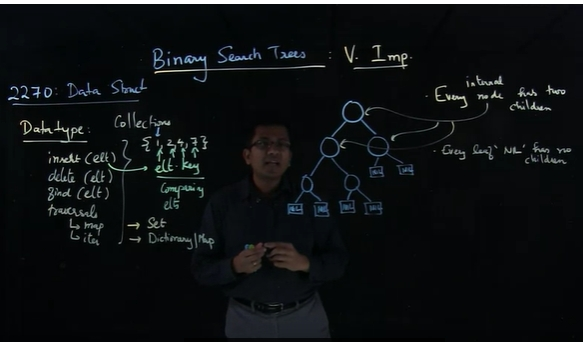
\includegraphics[width=\textwidth]{binarysearchtreenodes.png}
\end{figure}

\paragraph{
    When there is a node with the key 25, every node in the left subtree
    will have a key $<$ 25, and every node in the right subtree will
    have a key $>$ 25.\\
    The rule will also apply to all those subtrees.\\
}

\begin{figure}[H]
    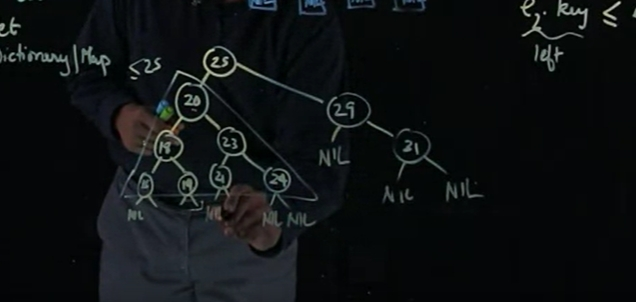
\includegraphics[width=\textwidth]{binarysearchtreerealexample.png}
\end{figure}

\begin{verbatim}
    Example:
     25
    /  \
   15  50
  / \  / \
 10 22 35 70
\end{verbatim}

\begin{verbatim}

Question:
Binary Search Trees may look similar to Heaps, but it is important 
to consider their differences.
In a Min-Heap, the smallest element must be the root node of the tree.
In a Binary Search Tree, on the other hand, how would we find the 
smallest element?

A: We would traverse the left subtree of the root node until we 
reach a leaf node, which means a node with a NIL as its left child.
\end{verbatim}


\subsection{The Height of a Binary Search Tree}

\paragraph{
    The height of a binary search tree is the number of edges on the
    longest path from the root node to a leaf node.\\
    We will define the height of a leaf node as 0. Then the height of number 25, 
    a.k.a. the root node of the below binary search tree is 2.\\
}

\newpage

\begin{verbatim}
    Example:
     25       -> height = 2
    /  \
   15  50     -> height = 1
  / \  / \
 10 22 35 70  -> height = 0, since they are leaf nodes
\end{verbatim}

\paragraph{
    Let's assume we have a balanced binary search tree with n internal nodes.\\
    One each layer from the root node, there'll be $2^0$ nodes, $2^1$ nodes, $2^2$ nodes, $\cdots$, $2^h$ nodes.\\
    The total number of nodes in the tree will be $2^0+2^1+2^2+ \cdots +2^h=2^{h+1}-1$.\\
    So, the height of the tree will be $h=\log_2(n+1)-1$.\\
    In the sense of big O notation, the height of a binary search tree is $O(\log_2(n))$, in a balanced binary 
    search tree scenario.\\
    For example, $\log_2^8=3$, so the height of a binary search tree with 8 nodes is 3.\\
    $\log_2^{15}=4$, so the height of a binary search tree with 15 nodes is 4.\\
}

\paragraph{
    In the worst case scenario, where the binary search tree is not balanced, the height of the tree will be $O(n)$.\\
    That is to say, the tree will be a linked list looks like this;\\
}

\newpage

\begin{verbatim}
    Linked List Example:
     10
      \
       15
        \
         20
          \
           25
            \
             30
              \
               35
\end{verbatim}

\paragraph{
    In this case, the height of the tree is 6, which is equal to the number of nodes in the tree.\\
    The height of the tree is $O(n)$, which is the worst case scenario.\\
    Normally, we will have something in between the best case scenario and the worst case scenario, 
    $O(\log(n)) < height < O(n)$.\\
}

\subsection{Basics of Binary Search Tree Quiz}

\begin{figure}[H]
    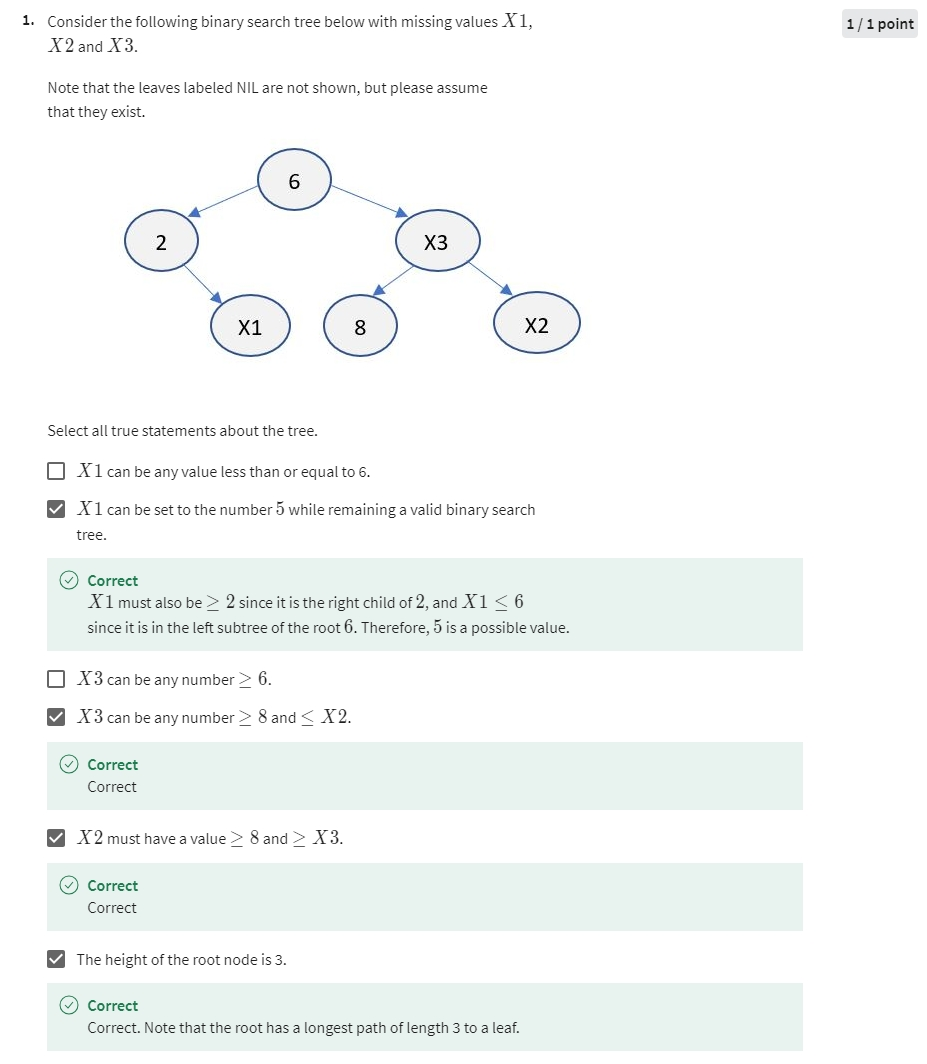
\includegraphics[width=\textwidth]{binarysearchtreequiz01.png}
\end{figure}

\begin{figure}[H]
    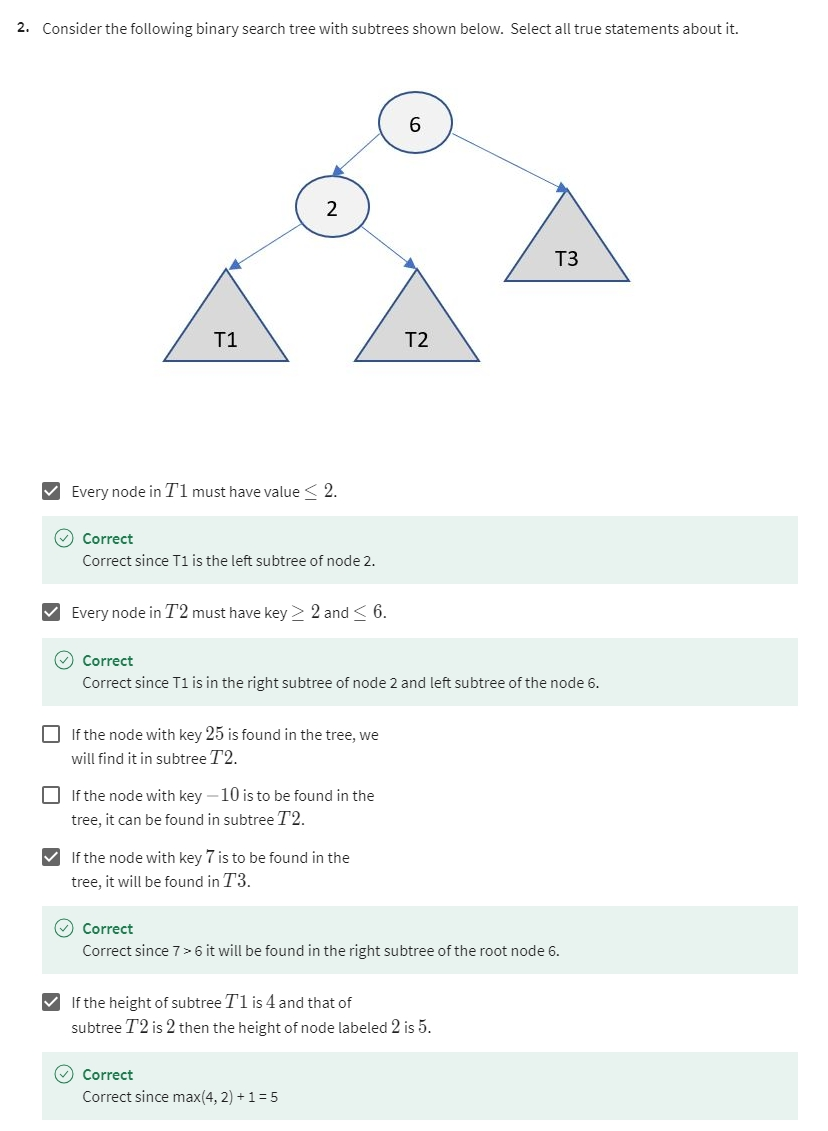
\includegraphics[width=\textwidth]{binarysearchtreequiz02.png}
\end{figure}

\begin{figure}[H]
    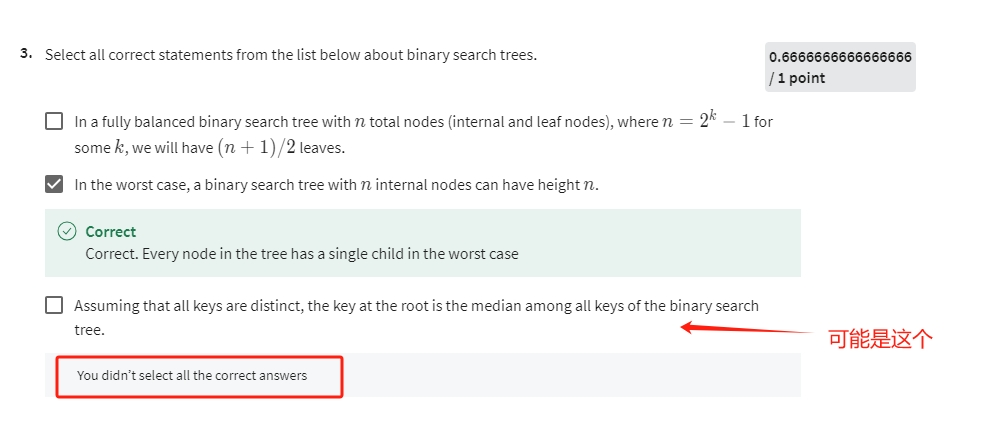
\includegraphics[width=\textwidth]{binarysearchtreequiz03.png}
\end{figure}



\subsection{Insertion and Deletion in a Binary Search Tree}

\subsubsection{Insertion}

\paragraph{
    We can insert a new element into a binary search tree by comparing the key of the new element with the key of the root node.\\
    If the key of the new element is less than the key of the root node, we will insert the new element into the left subtree.\\
    If the key of the new element is greater than the key of the root node, we will insert the new element into the right subtree.\\
    We will repeat the process until we reach a leaf node.\\
    For example, we have a binary search tree with the following nodes;\\
}

\begin{verbatim}
    Example:
     25
    /  \
   15  50
  / \  / \
 10 22 35 70
\end{verbatim}

\paragraph{
    If we want to insert a new element with the key 40, we will compare 40 with 25, and then 40 with 50, and then 40 with 35.\\
    Since 40 is greater than 35, we will insert 40 as the right child node of 35.\\
}

\paragraph{
    The above example actually consists of two steps.\\
    First, we will search for the element to be inserted, which is called the $find()$ operation.\\
    Then, after successfully locates the element, we will insert it into the binary search tree.\\
    We will talk about find operation now.\\
    Assuming we have an impefect binary search tree and we want to locate the key $45$, how should we do that?\\
}

\begin{figure}[H]
    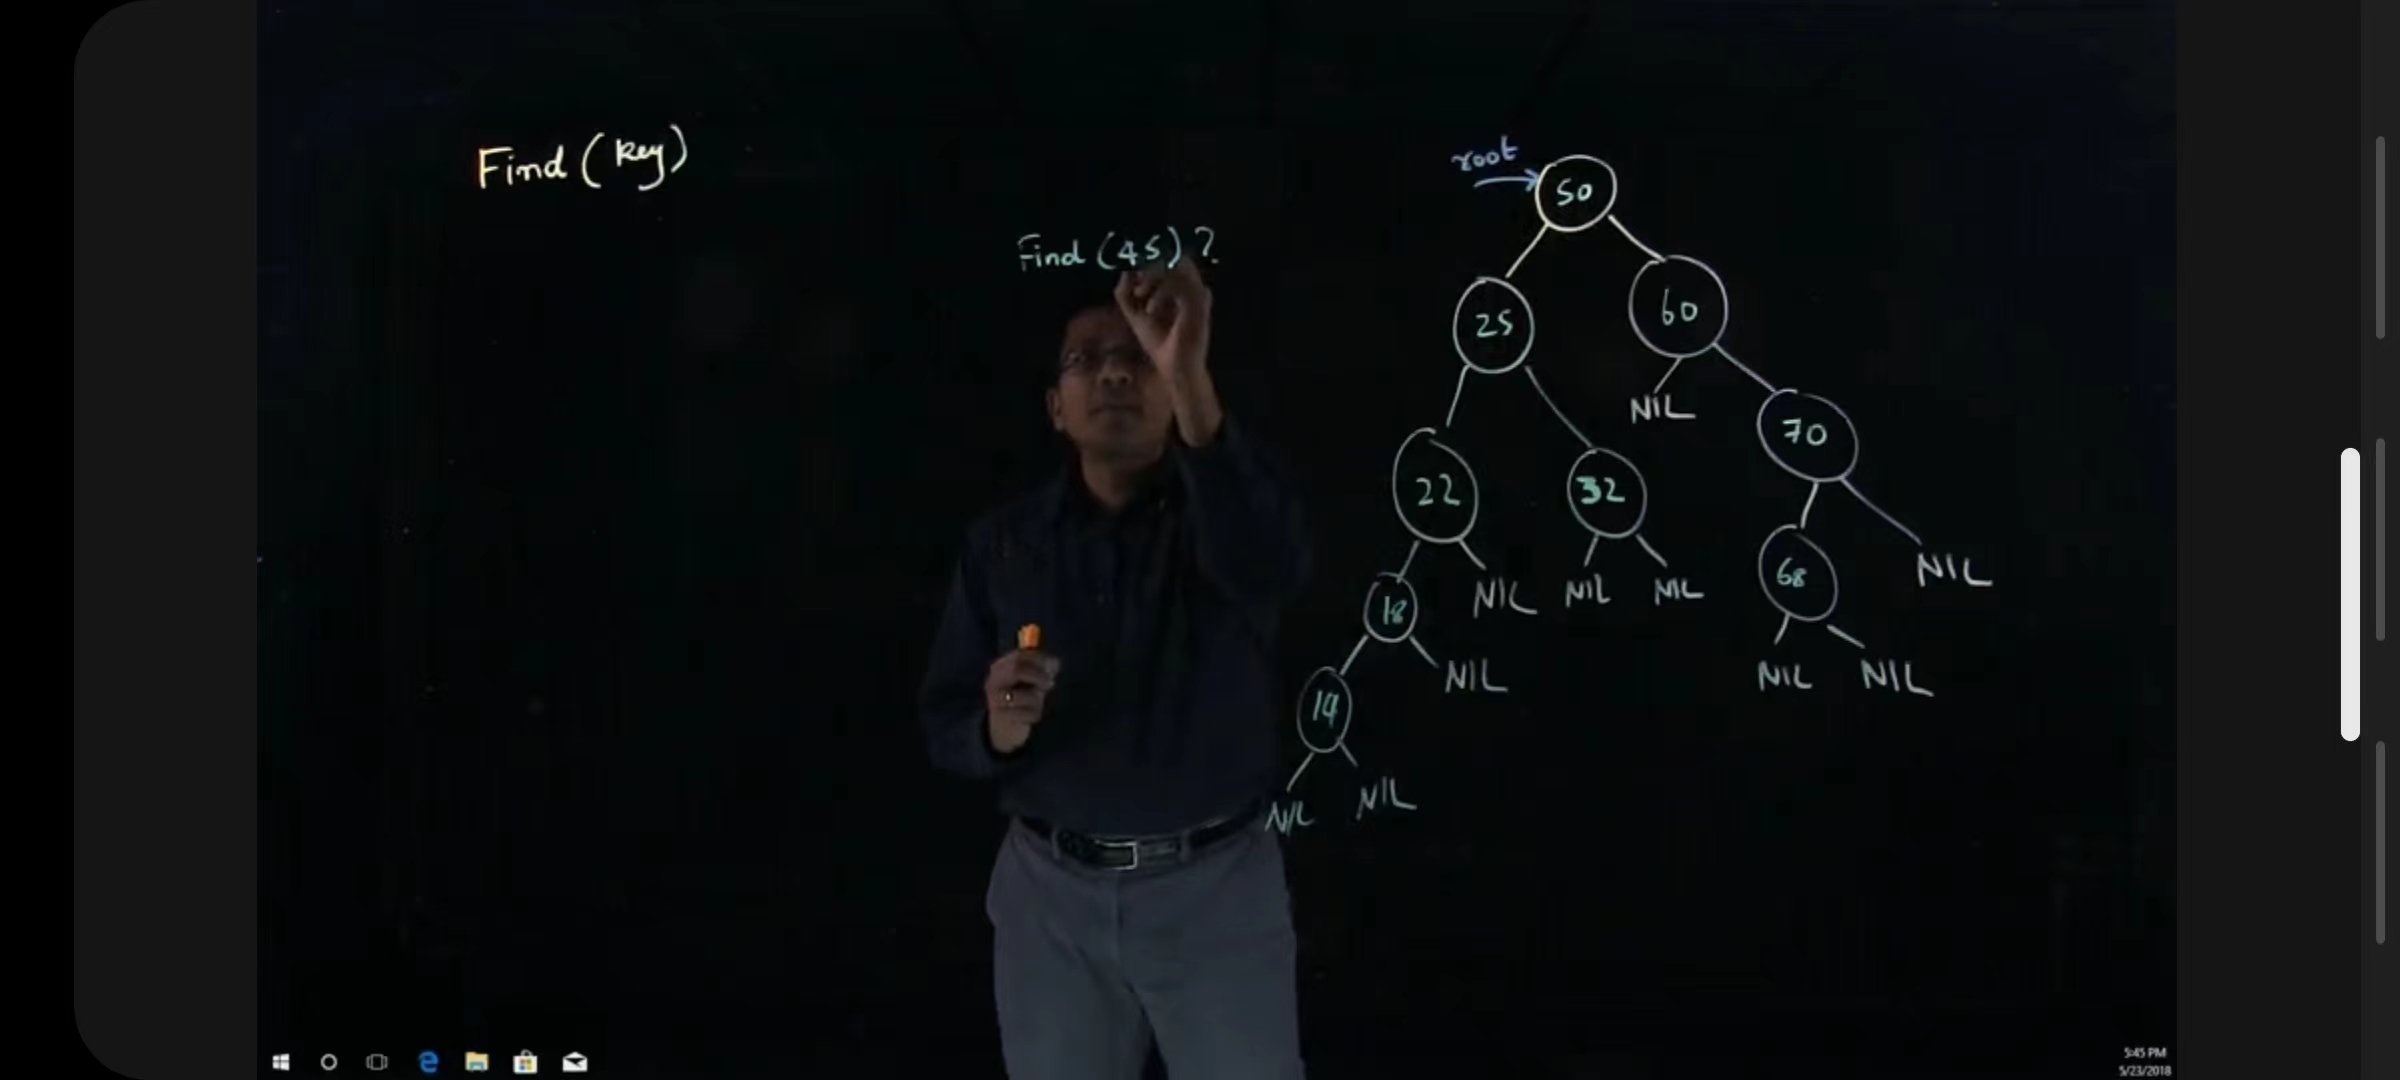
\includegraphics[width=\textwidth]{binarysearchtreeinsertion.jpg}
\end{figure}

\paragraph{
    We will start from the root node, and then compare the key of the root node with the key of the element to be located.\\
    If the key of the root node is equal to the key of the element to be located, we will return the root node. 
    If the key of the root node is greater than the key of the element to be located, we will search the left subtree. 
    Otherwise, we will search the right subtree.\\
    The overall process will be repeated until we reach a leaf node.\\
    If we reach a leaf node and the key of the leaf node is not equal to the key of the element to be located, we will return NIL.\\
}

\begin{verbatim}
    Here is the pseudo code for the find operation:
    find(root, key)
        if root == NIL or root.key == key
            return root
        if root.key > key
            return find(root.left, key) # This is the recursive call.
        return find(root.right, key) # This is the recursive call.
\end{verbatim}

\paragraph{
    As for the time complexity, the find operation will take $O(h)$ time, where $h$ is the height of the binary search tree.\\
    Now we will go ahead with the second step of the insertion operation.\\
    We will insert the new element into the binary search tree by comparing the key of the new element with the key of the root node.\\
    }

\begin{verbatim}
    Here is the pseudo code for the insertion operation:
    insert(root, key)
        if root == NIL
            return new Node(key)
        if key < root.key
            root.left = insert(root.left, key) # This is the recursive call.
        else
            root.right = insert(root.right, key) # This is the recursive call.
        return root
\end{verbatim}

\begin{figure}[H]
    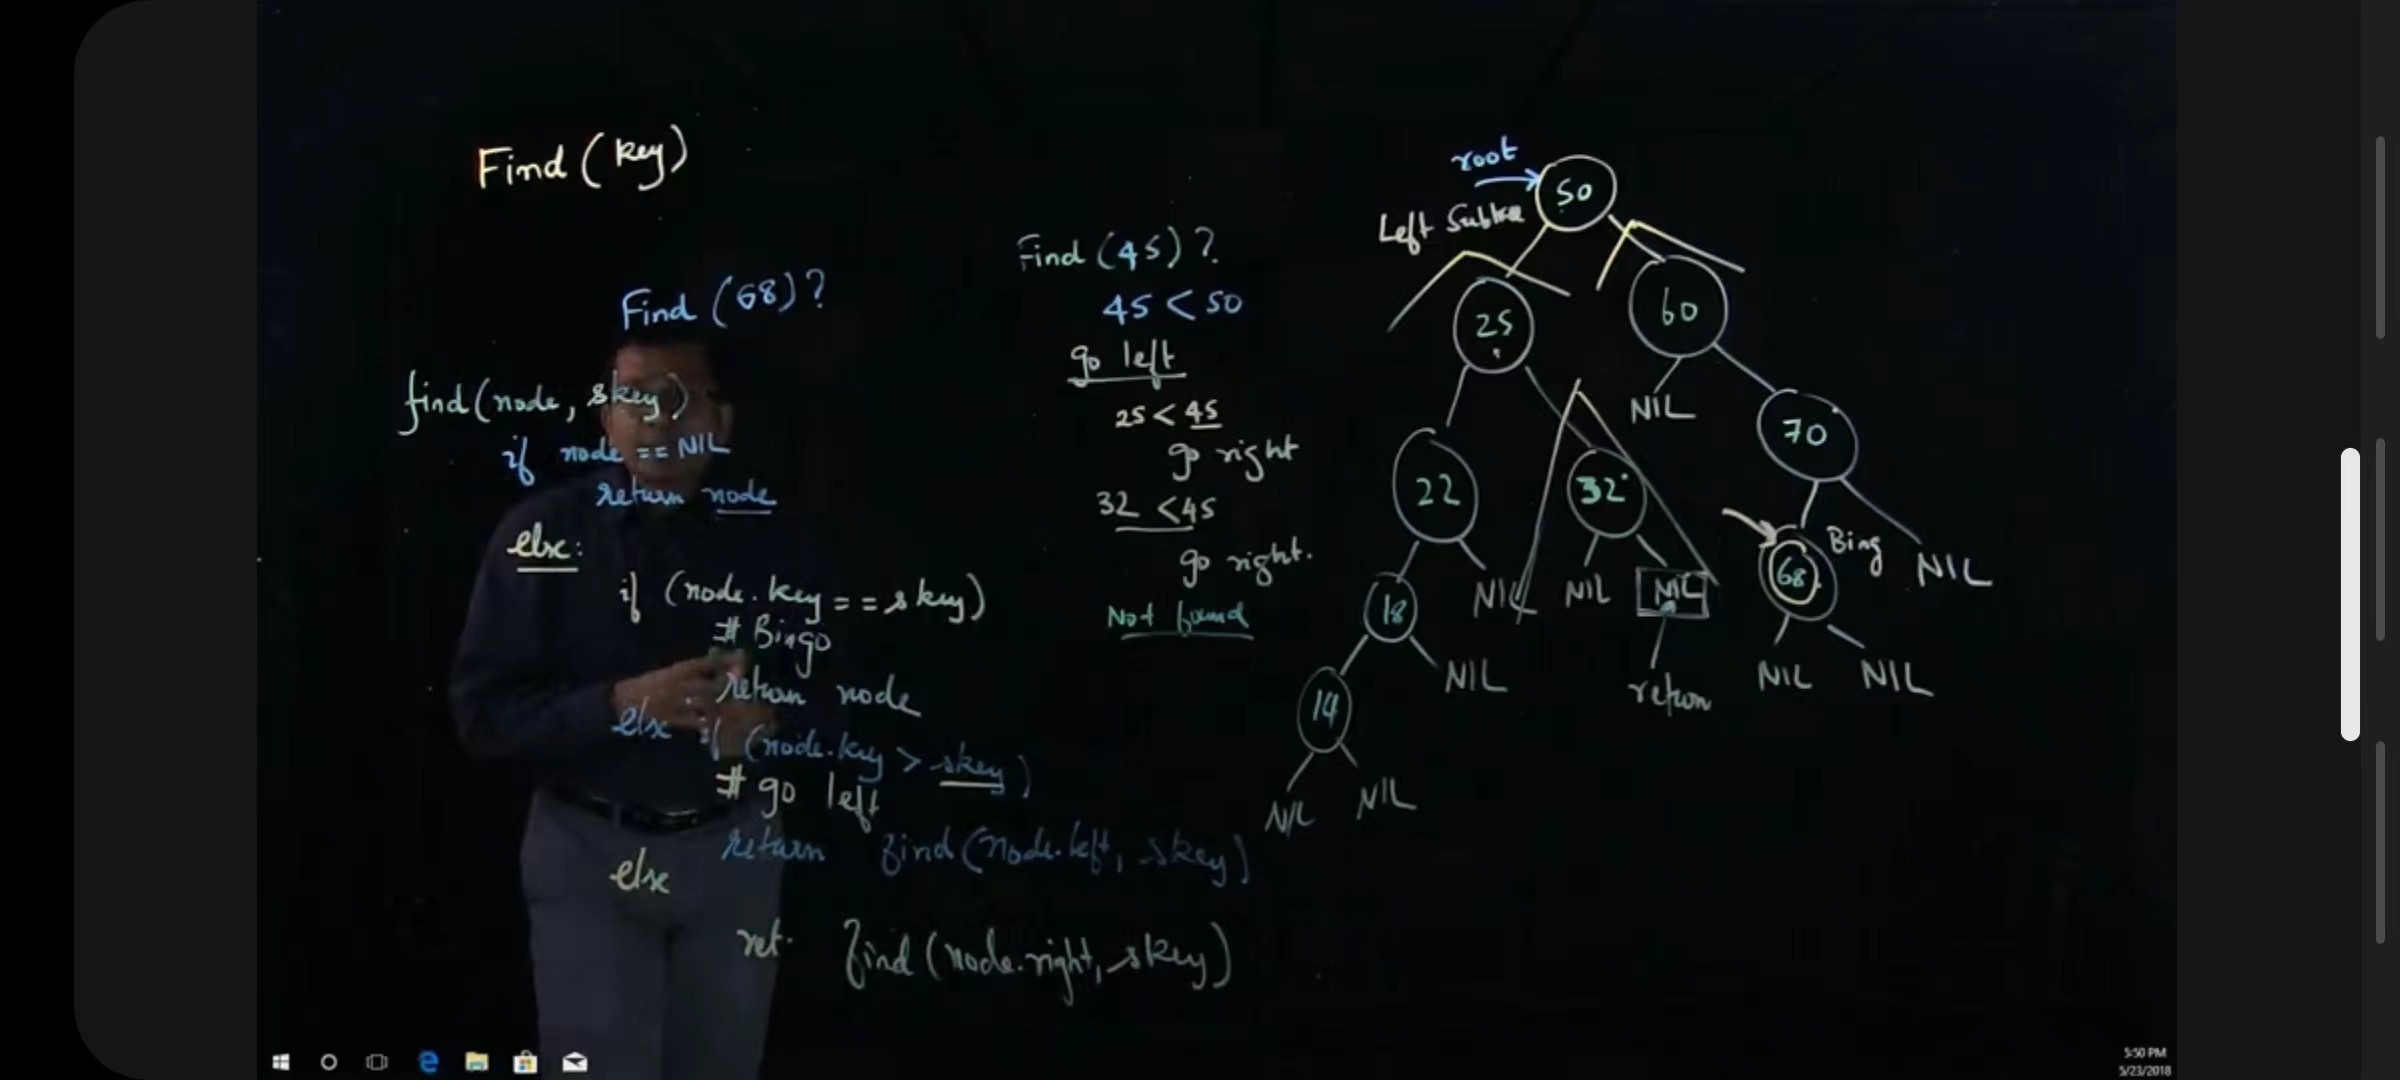
\includegraphics[width=\textwidth]{binarysearchtreeinsertion2.jpg}
\end{figure}

\subsubsection{Deletion}

\paragraph{
    Now we will talk about the deletion operation.\\
    There are three cases to consider when deleting a node from a binary search tree.\\
    The node to be deleted can be a leaf node, a node with only one child,or one with two child nodes.\\
    If both child nodes are NIL, we can simply delete the node.\\
    If one of the child nodes is NIL, we can delete the node, then reconnect between the past-parrent node and past-child node,
     like this;\\
}

\newpage

\begin{verbatim}
    Only One Child Node Example:
     25                     25
    /  \                   /  \
   15  50   delete 15     /   50
  / \       --------->   / \
 10 NIL                 10  NIL
 /\                    / \
NIL NIL               NIL NIL
\end{verbatim}

\paragraph{
    What if we want to delete a node that has two non-NIL children?\\
    We will find the smallest node in the right subtree of the node to be deleted, and then replace the node to be deleted with the smallest node.\\
    To perform this operation, we will `walk' right from the root node by one step and then `walk' left until we reach a leaf node.\\
    During each step, we will compare the key of the current node with the key of the node to be deleted.\\
    The leaf node we reached will be the successor of the node we deleted.\\
}

\begin{verbatim}
    Two Child Nodes Example:
     25                     25
    /  \                   /  \
   15  50   delete 15     22   50
  / \       --------->   / \
 10 22                 10  NIL
 /\                    / \
NIL NIL               NIL NIL
\end{verbatim}

\begin{verbatim}
    Here is the pseudo code for the deletion operation:
    delete(root, key)
        if root == NIL
            return root
        if key < root.key
            root.left = delete(root.left, key) # This is the recursive call.
        else if key > root.key
            root.right = delete(root.right, key) # This is the recursive call.
        else
            if root.left == NIL
                return root.right
            else if root.right == NIL
                return root.left
            root.key = minValue(root.right)
            root.right = delete(root.right, root.key) # This is the recursive call.
        return root
\end{verbatim}


\subsubsection{Tree Traversal}

\paragraph{
    There are three ways to traverse a binary search tree.\\
    In-order traversal, pre-order traversal, and post-order traversal.\\
    Inorder traversal visits nodes in a binary tree in the following order:\\
    Visit the left subtree.\\
    Visit the root node.\\
    Visit the right subtree.\\
    This traversal method is particularly useful for binary search trees (BSTs) because it visits the nodes in ascending order.\\
}

\begin{verbatim}
    Example:
    Consider the following binary search tree (BST):
       4
      / \
     2   6
    / \ / \
    1  3 5  7
    Inorder traversal of this tree would be: 1, 2, 3, 4, 5, 6, 7.

    Python Code:
    class Node:
        def __init__(self, key):
            self.left = None
            self.right = None
            self.val = key

    def inorder_traversal(root):
        if root:
            # Traverse the left subtree
            inorder_traversal(root.left)
            # Visit the root node
            print(root.val, end=' ')
            # Traverse the right subtree
            inorder_traversal(root.right)
\end{verbatim}

\paragraph{
    Preorder traversal visits nodes in the following order:\\
    Visit the root node.\\
    Visit the left subtree.\\
    Visit the right subtree.\\
    Preorder traversal is useful for creating a copy of the tree or getting a prefix expression of an expression tree.\\
}

\begin{verbatim}
    Example:
    Consider the same BST:
       4
      / \
     2   6
    / \ / \
    1  3 5  7
    Preorder traversal of this tree would be: 4, 2, 1, 3, 6, 5, 7.

    Python Code:
    def preorder_traversal(root):
        if root:
            # Visit the root node
            print(root.val, end=' ')
            # Traverse the left subtree
            preorder_traversal(root.left)
            # Traverse the right subtree
            preorder_traversal(root.right)
\end{verbatim}

\paragraph{
    Postorder traversal visits nodes in the following order:\\
    Visit the left subtree.\\
    Visit the right subtree.\\
    Visit the root node.\\
    Postorder traversal is useful for deleting a tree or evaluating postfix expressions of an expression tree.\\
}

\begin{verbatim}
    Example:
    Consider the same BST:
       4
      / \
     2   6
    / \ / \
    1  3 5  7
    Postorder traversal of this tree would be: 1, 3, 2, 5, 7, 6, 4.

    Python Code:
    def postorder_traversal(root):
        if root:
            # Traverse the left subtree
            postorder_traversal(root.left)
            # Traverse the right subtree
            postorder_traversal(root.right)
            # Visit the root node
            print(root.val, end=' ')
\end{verbatim}


\subsection{BST Quiz}

\begin{figure}[H]
    \centering
    \subfigure{
        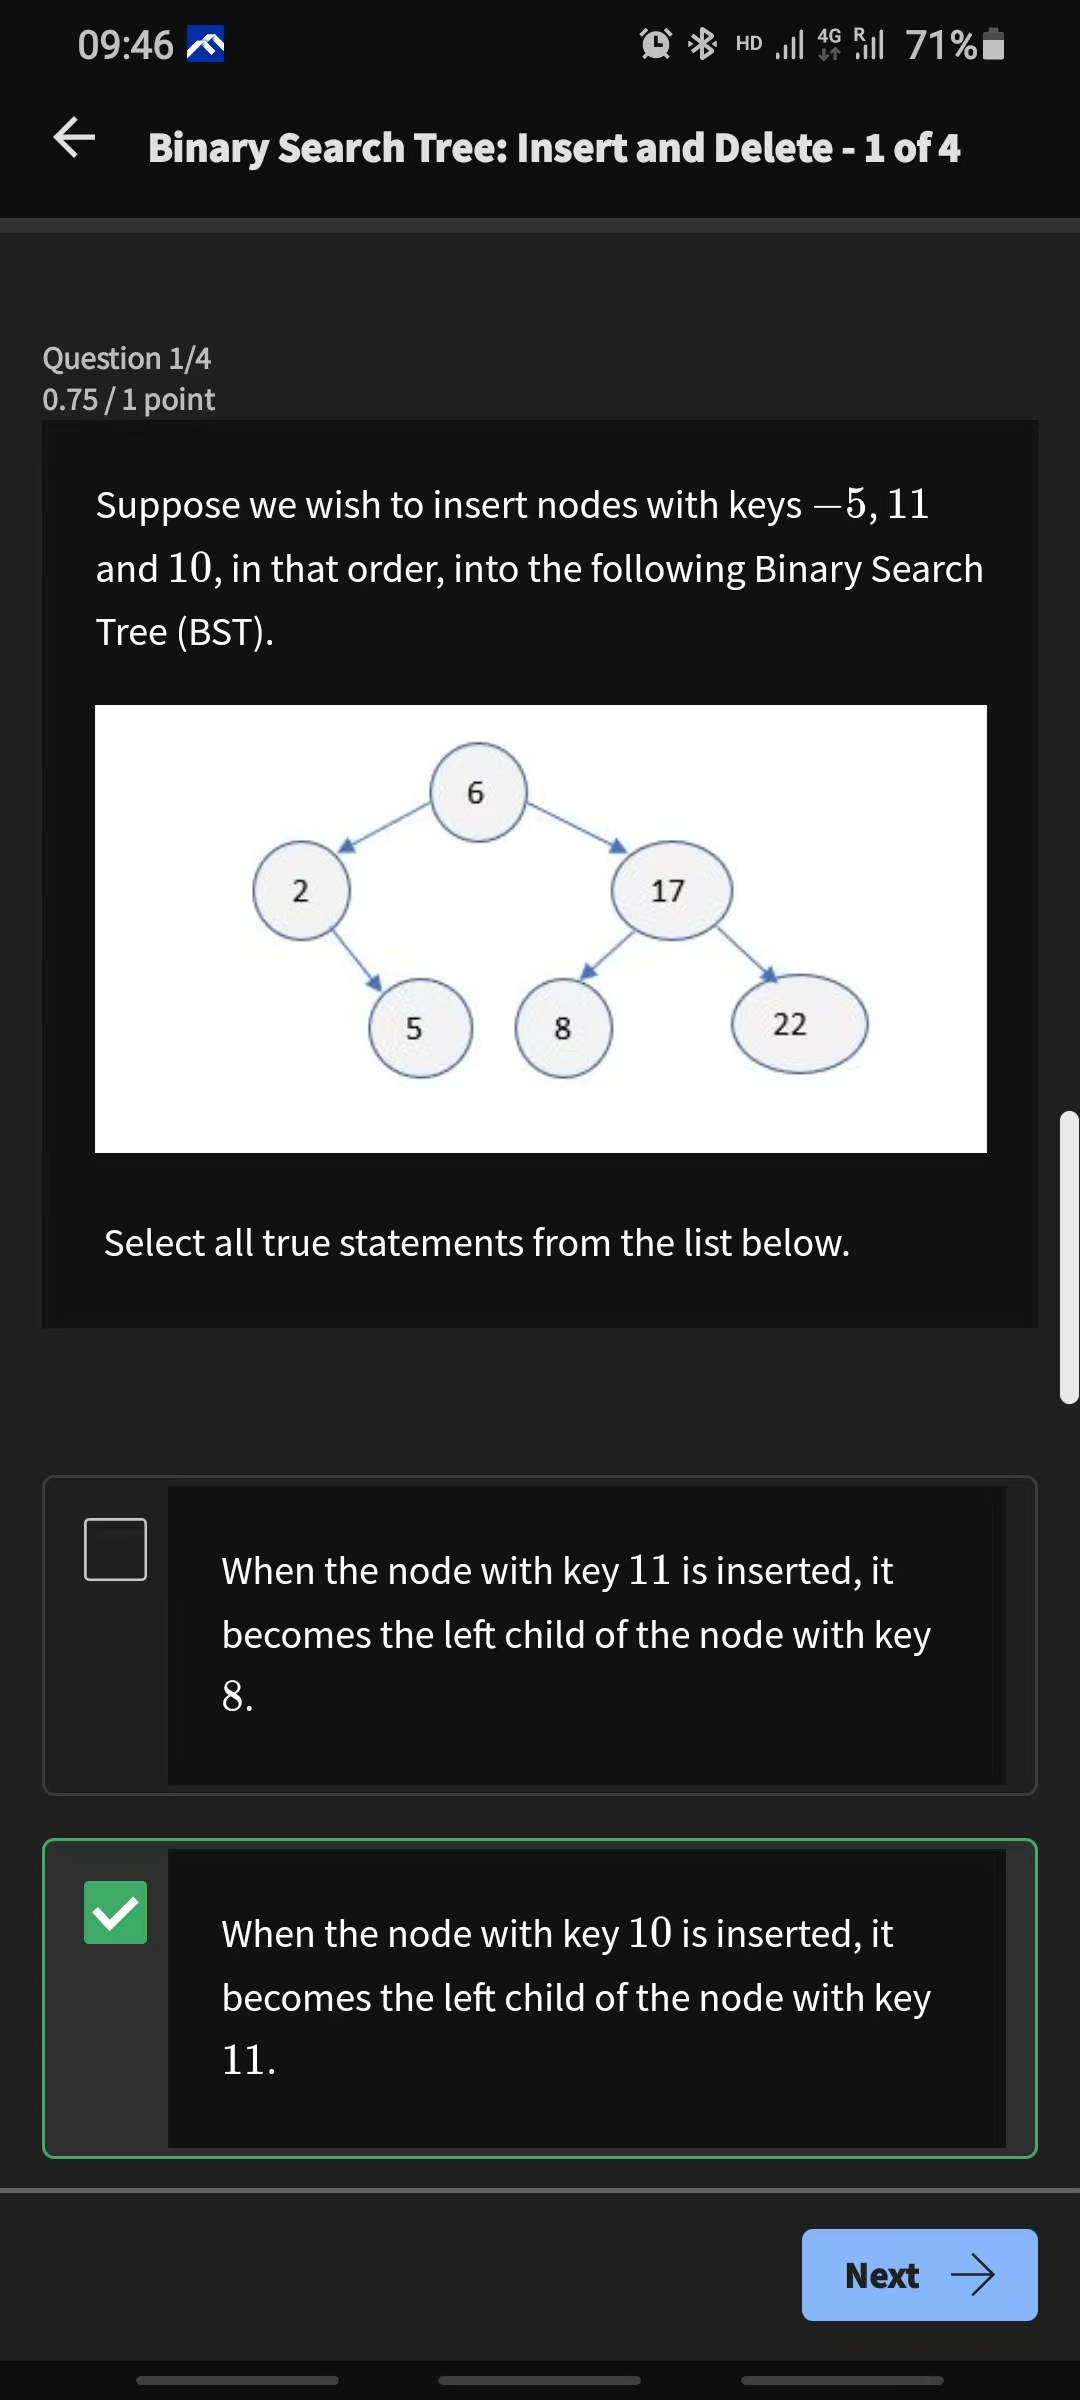
\includegraphics[width=0.45\textwidth]{bstinsertiondeletionquiz1-1.jpg}
    }
    \subfigure{
        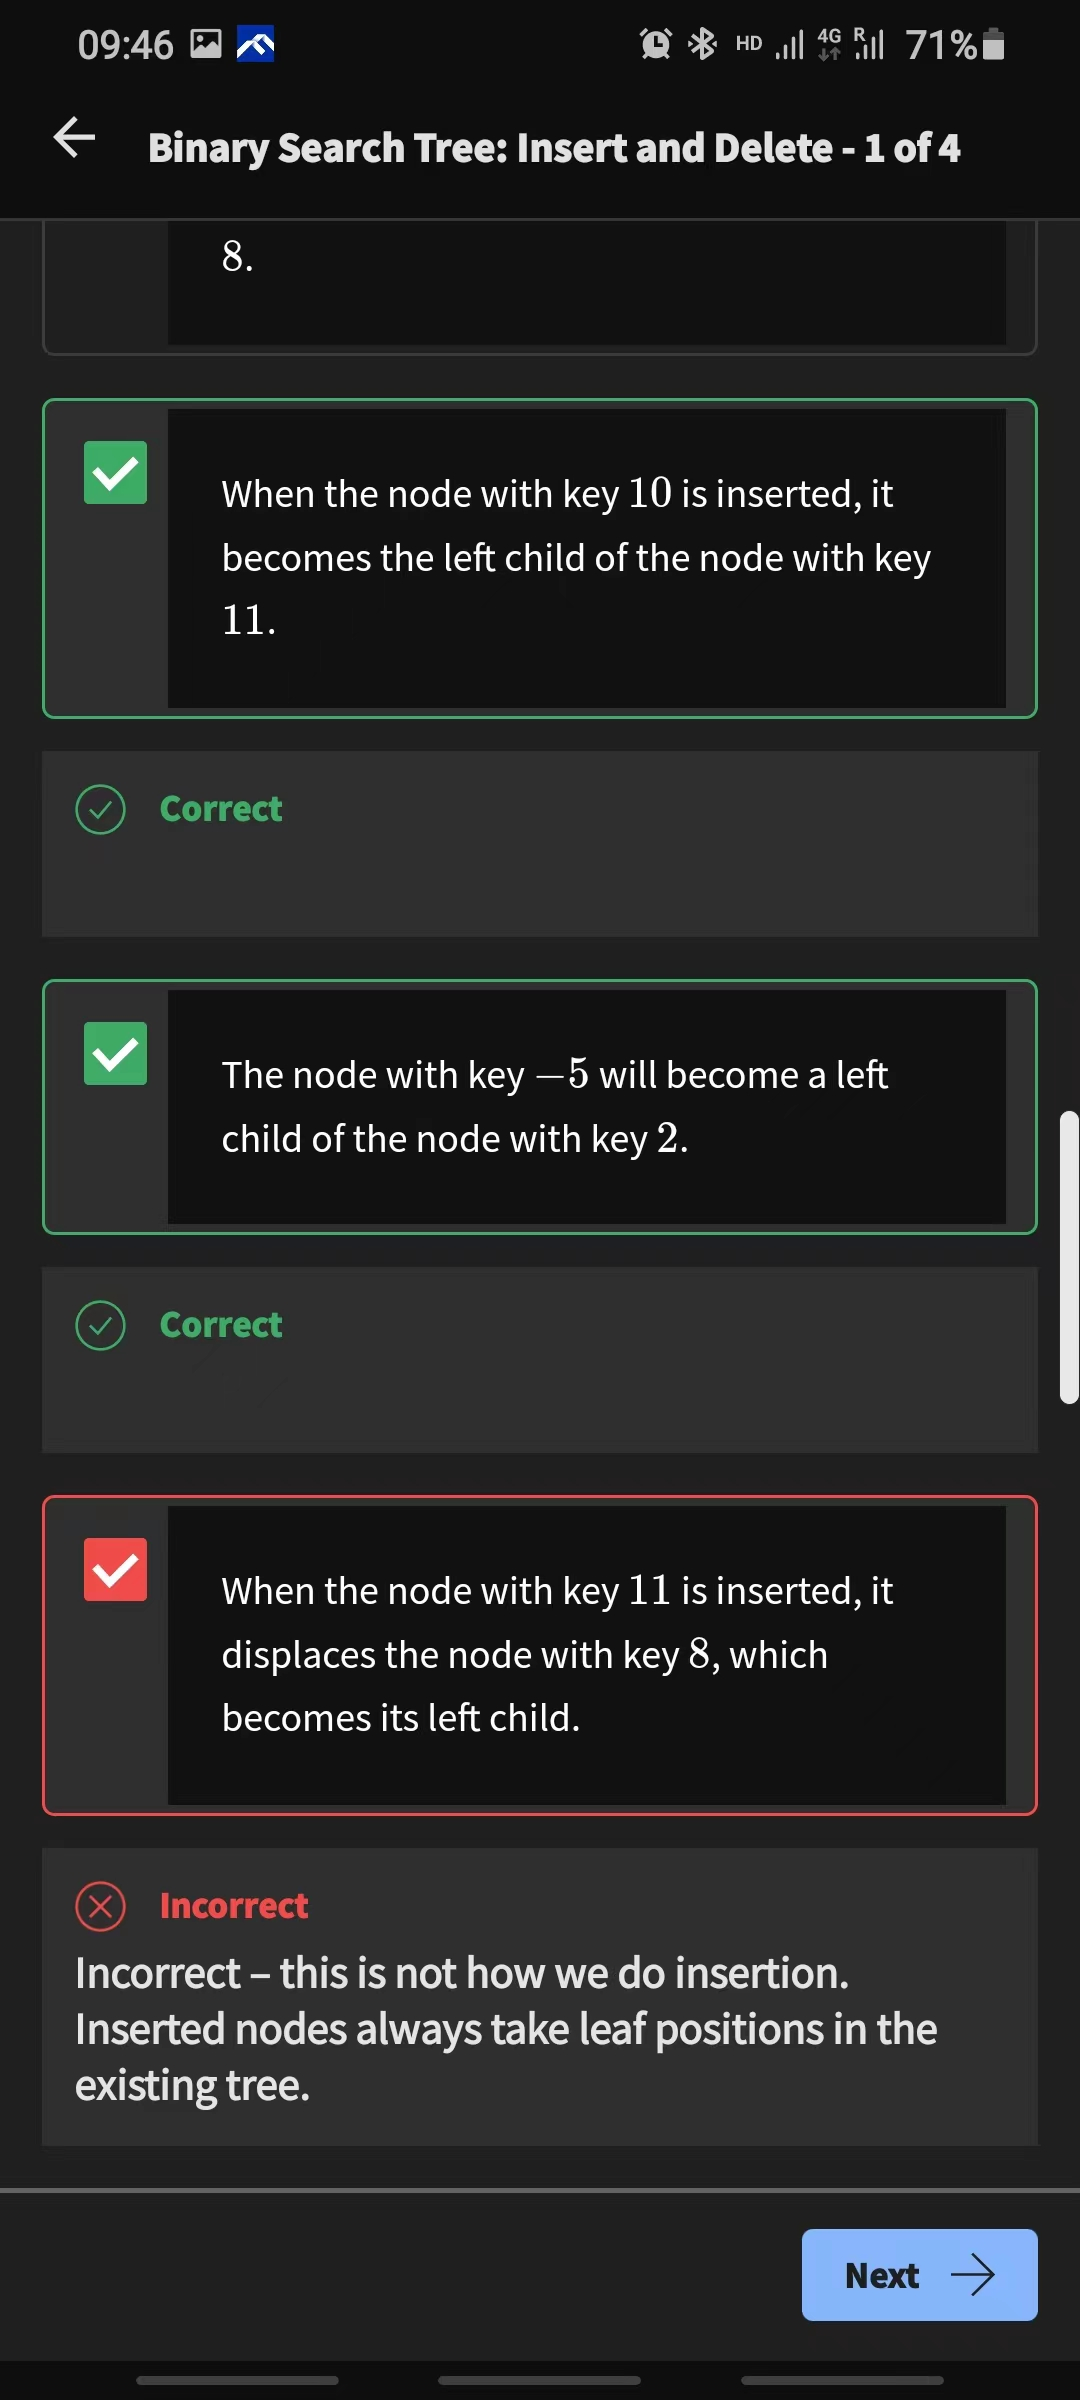
\includegraphics[width=0.45\textwidth]{bstinsertiondeletionquiz1-2.jpg}
    }
    \caption{Question 1}
    \label{fig:sidebyside}
\end{figure}

\begin{figure}[H]
    \centering
    \subfigure{
        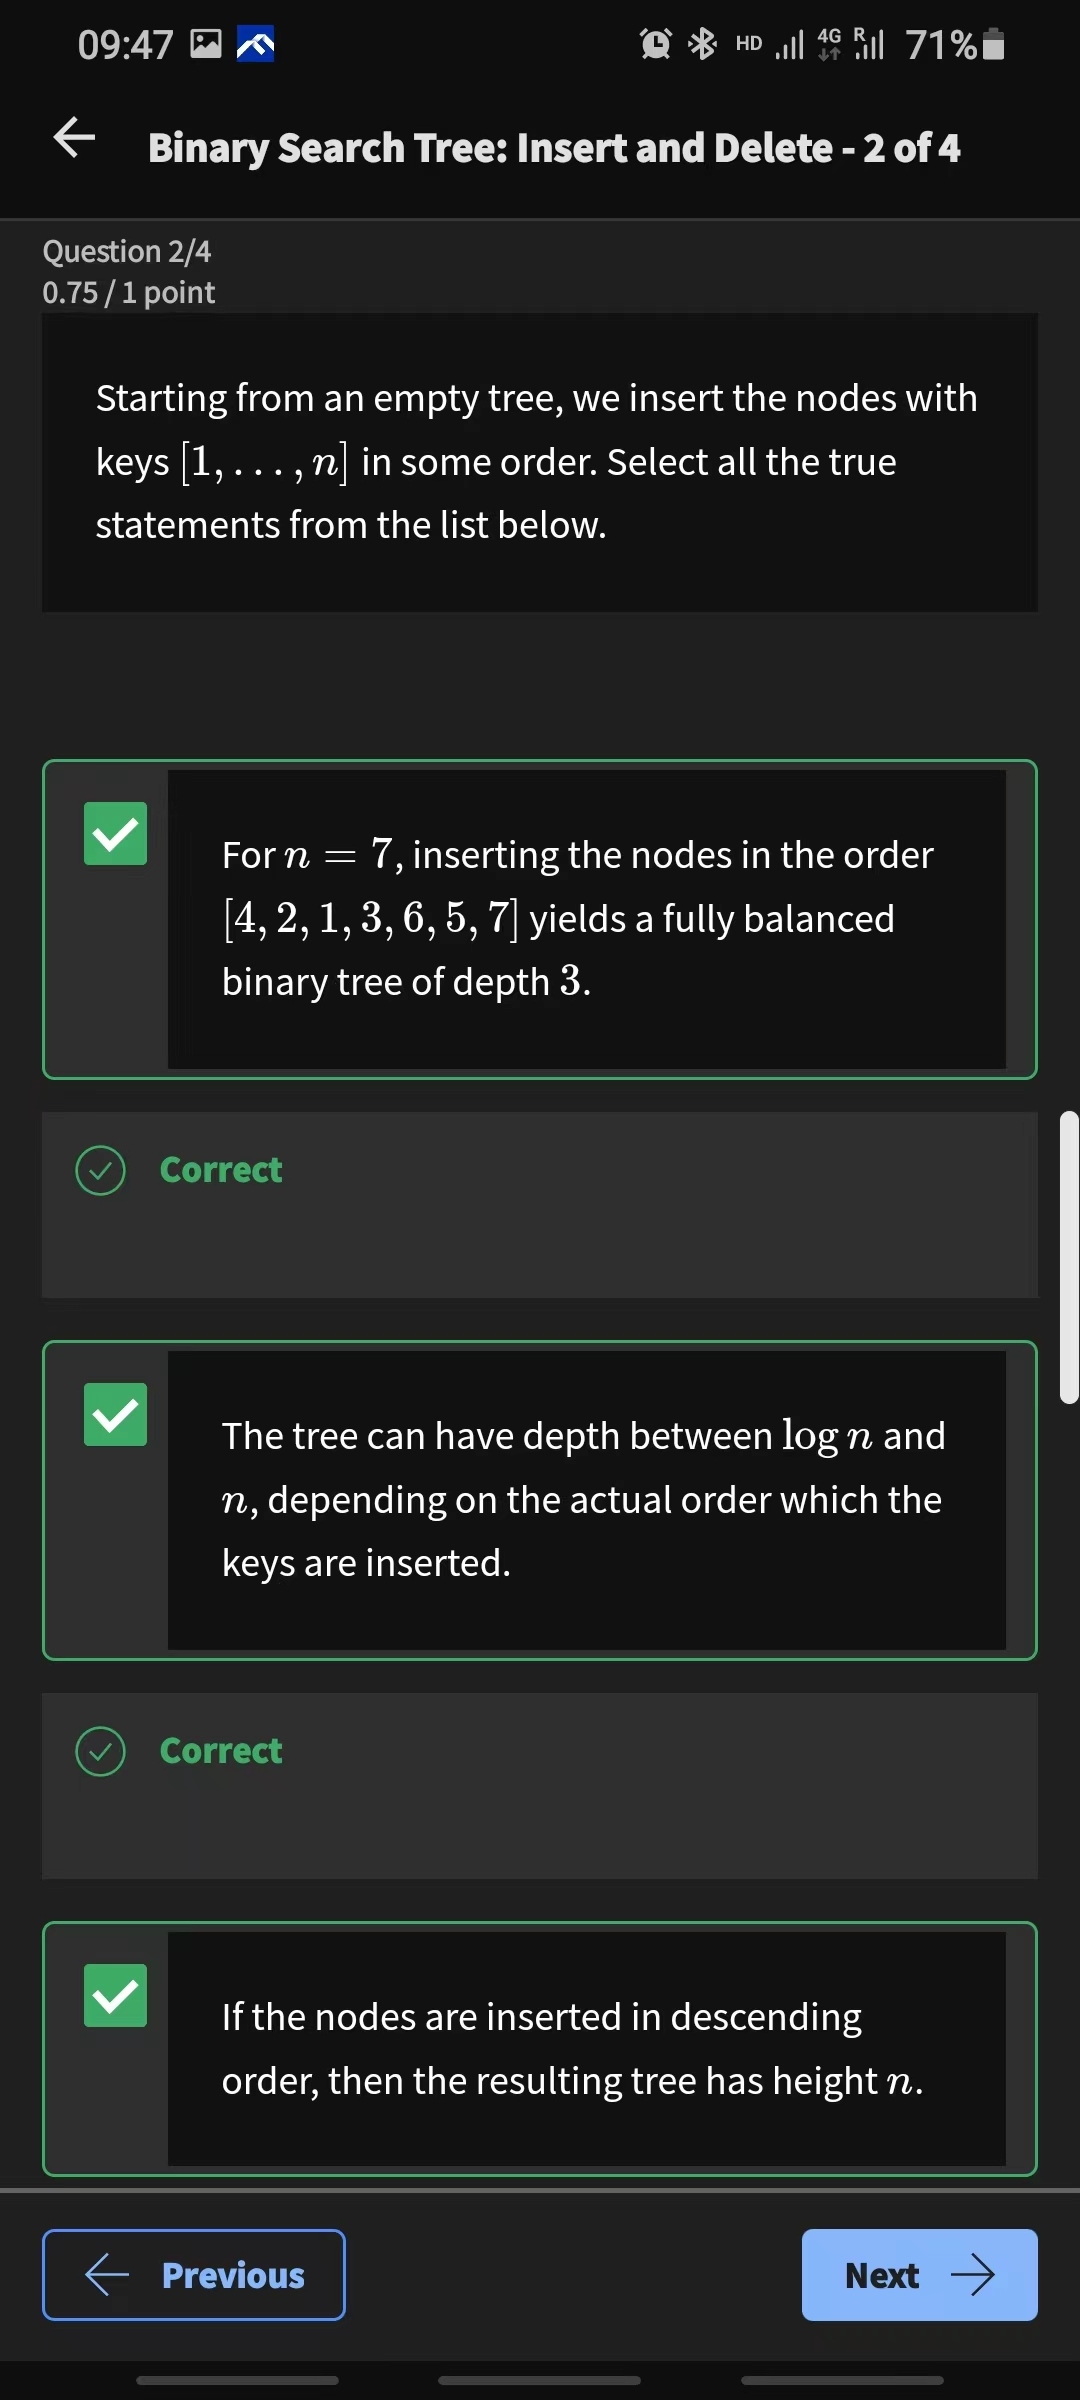
\includegraphics[width=0.45\textwidth]{bstinsertiondeletionquiz2-1.jpg}
    }
    \subfigure{
        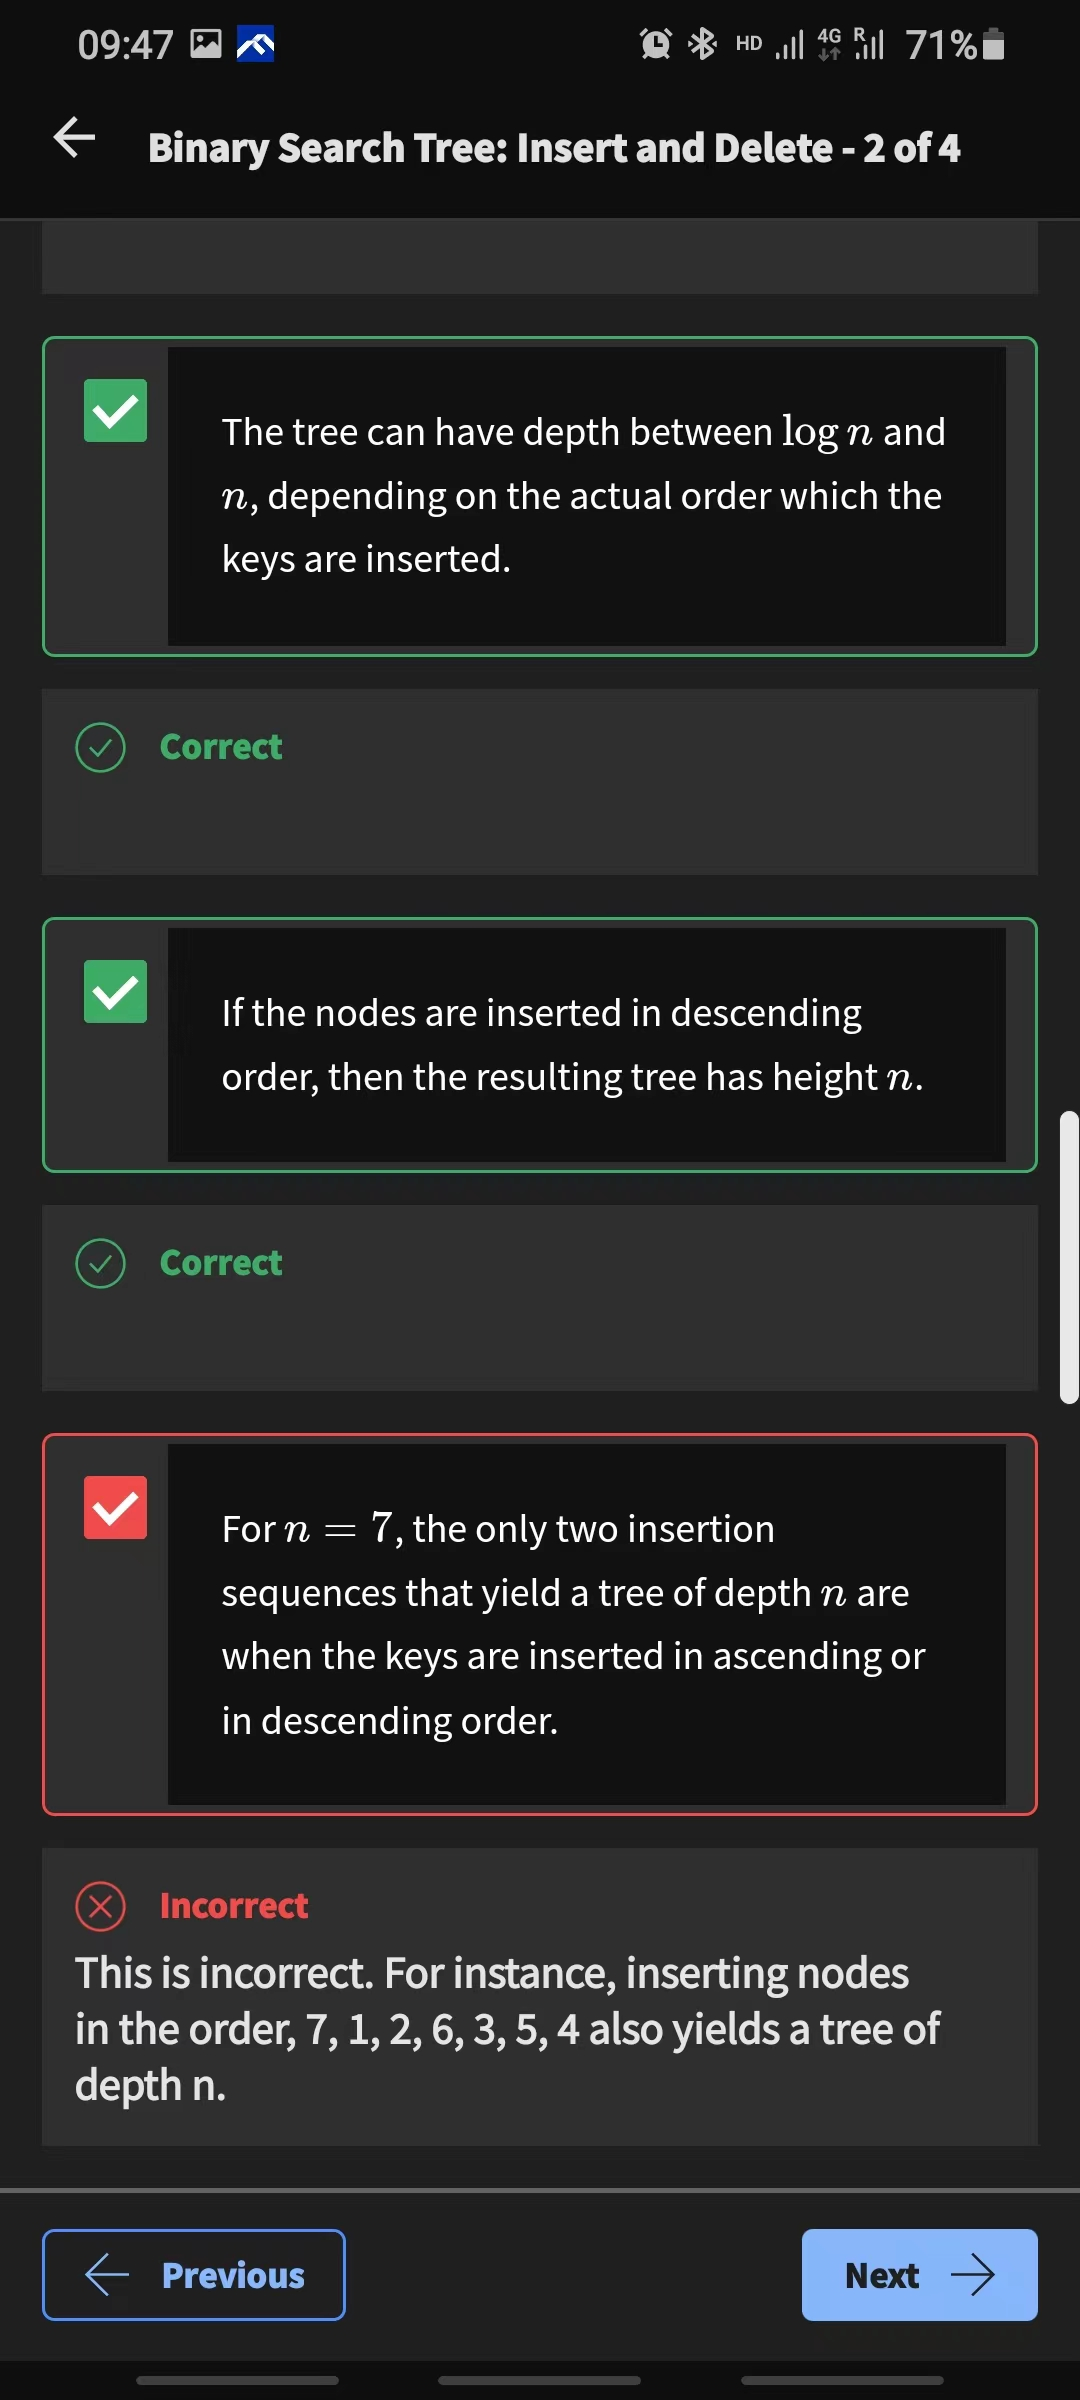
\includegraphics[width=0.45\textwidth]{bstinsertiondeletionquiz2-2.jpg}
    }
    \caption{Question 2}
    \label{fig:sidebyside}
\end{figure}


\begin{figure}[H]
    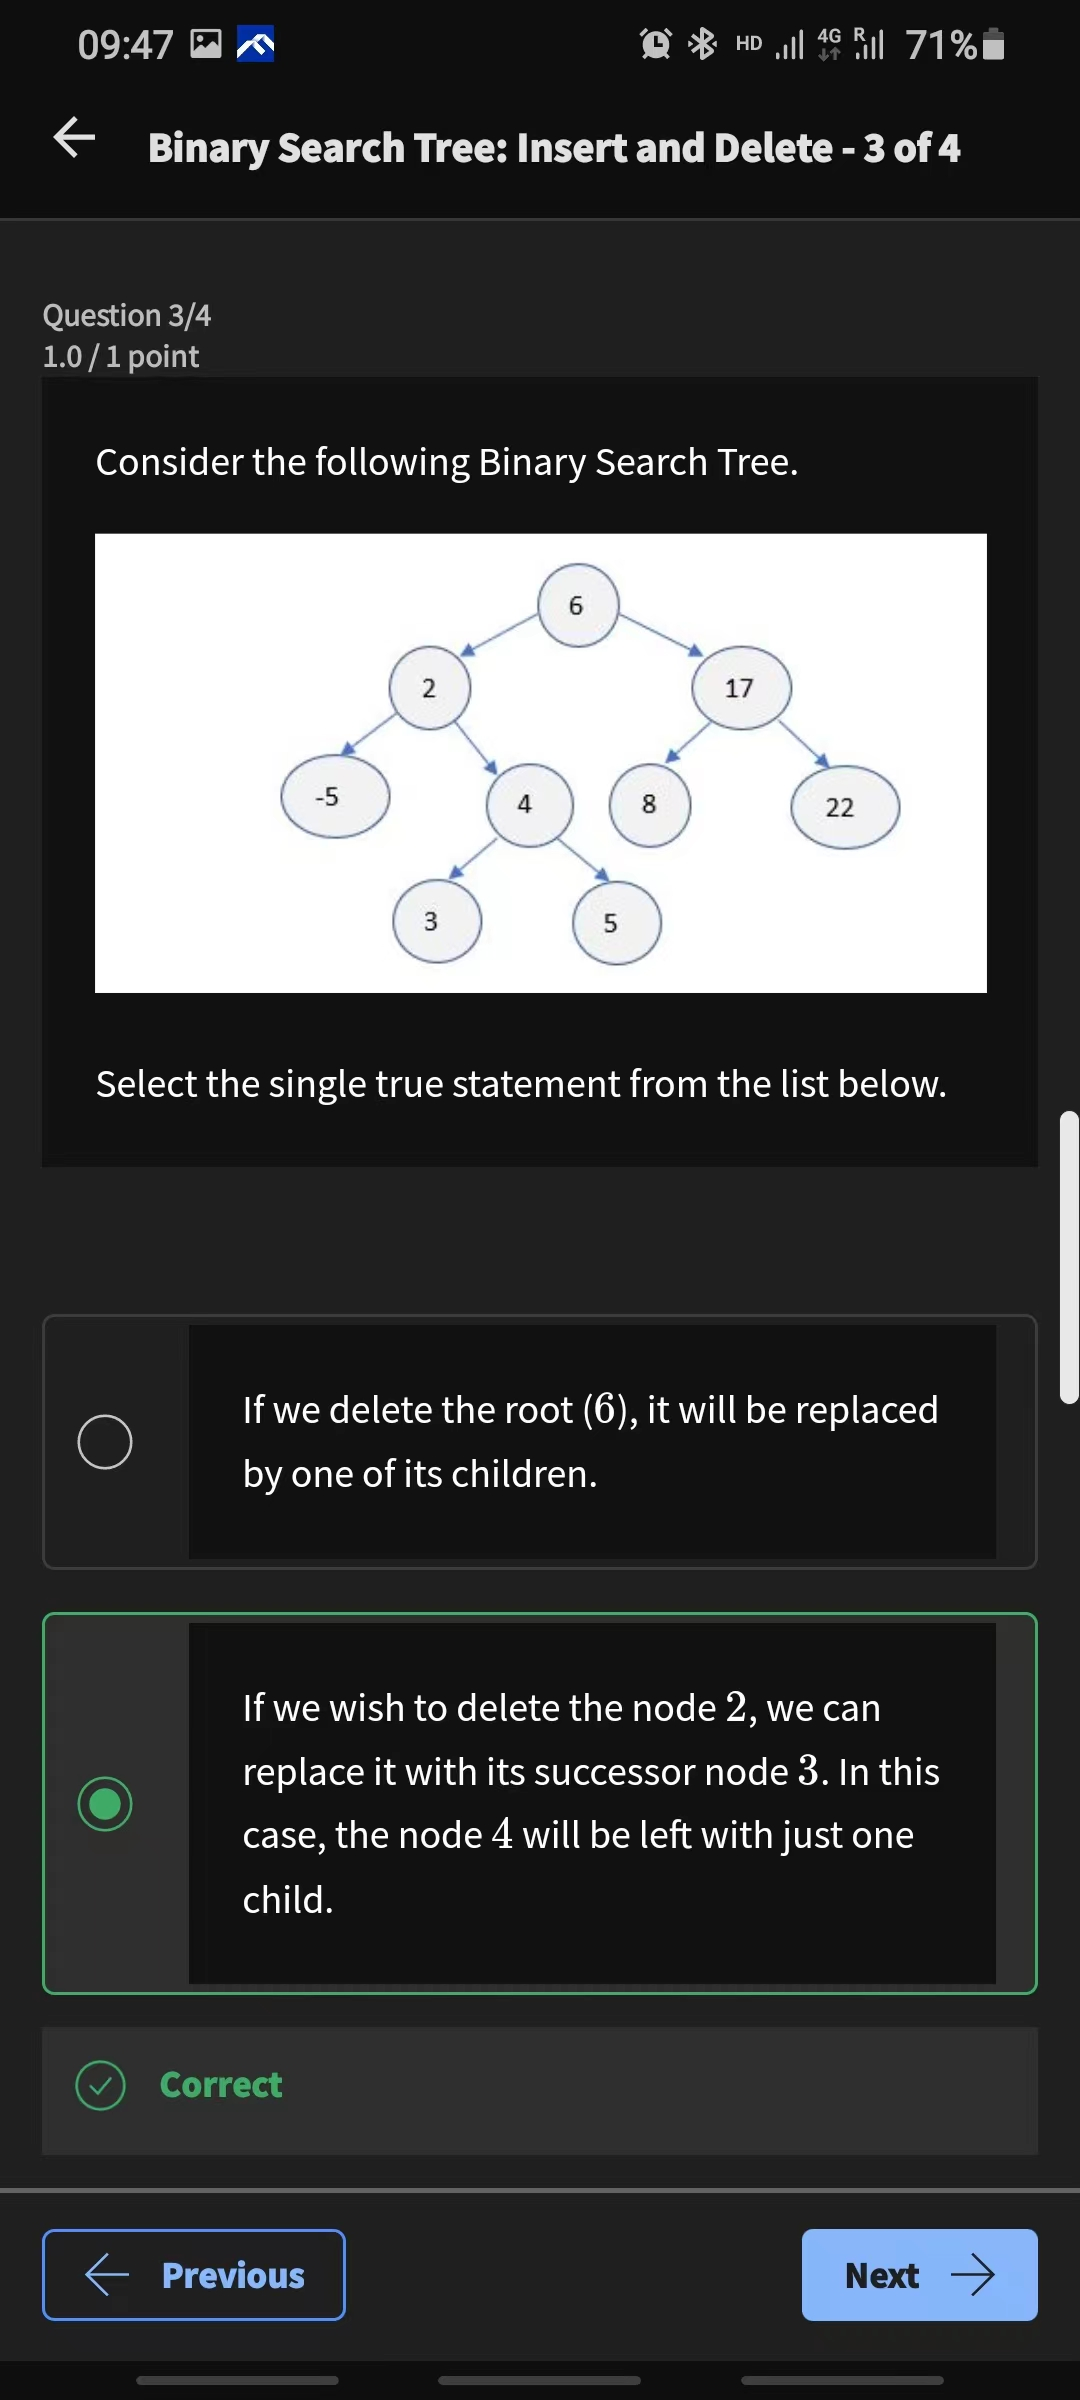
\includegraphics[width=\textwidth]{bstinsertiondeletionquiz3.jpg}
    \caption{Question 3}
\end{figure}


\begin{figure}[H]
    \centering
    \subfigure{
        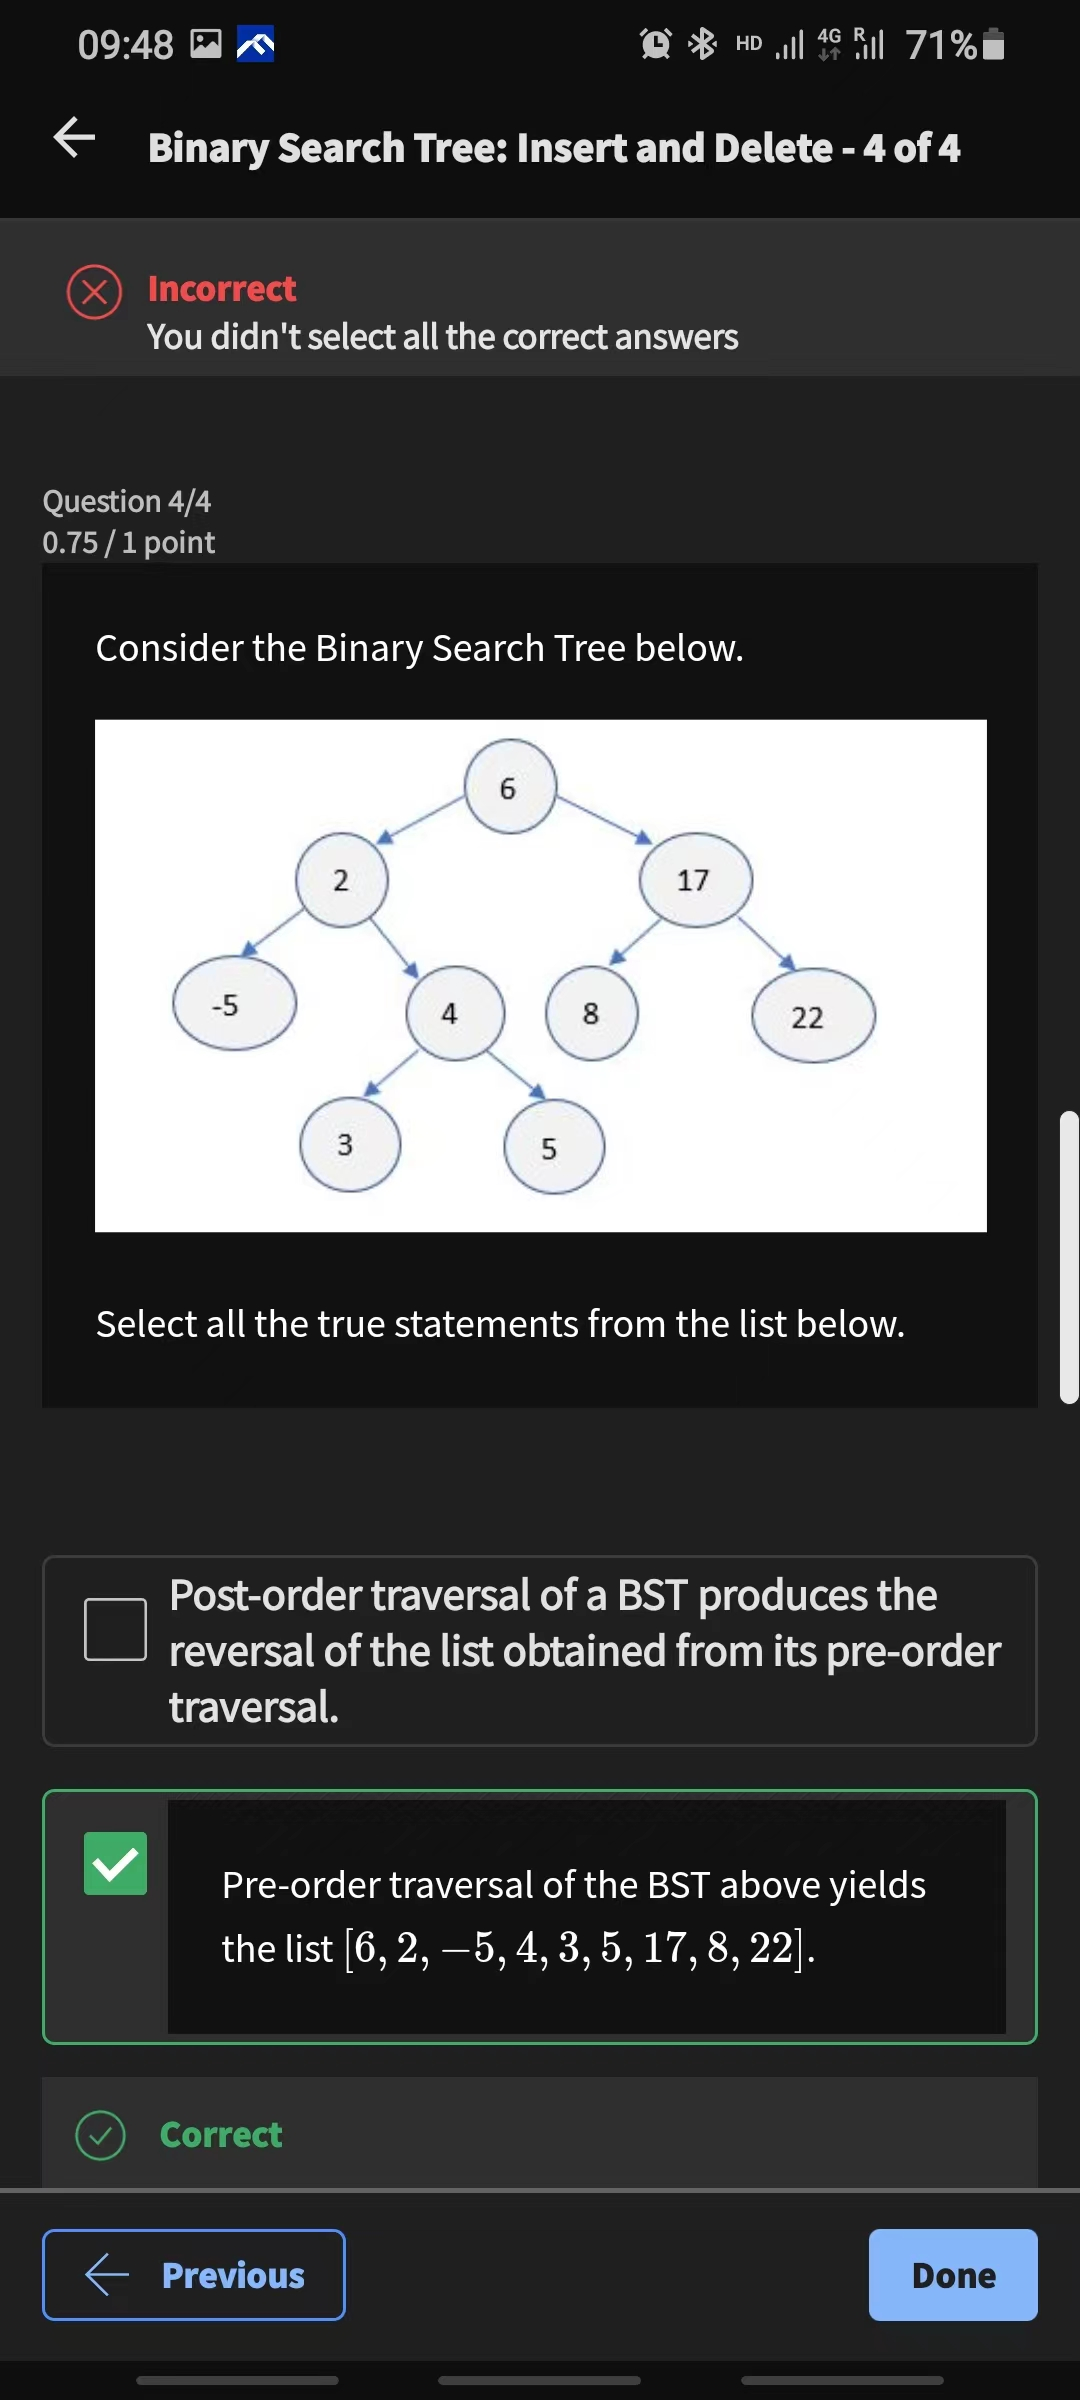
\includegraphics[width=0.45\textwidth]{bstinsertiondeletionquiz4-1.jpg}
    }
    \subfigure{
        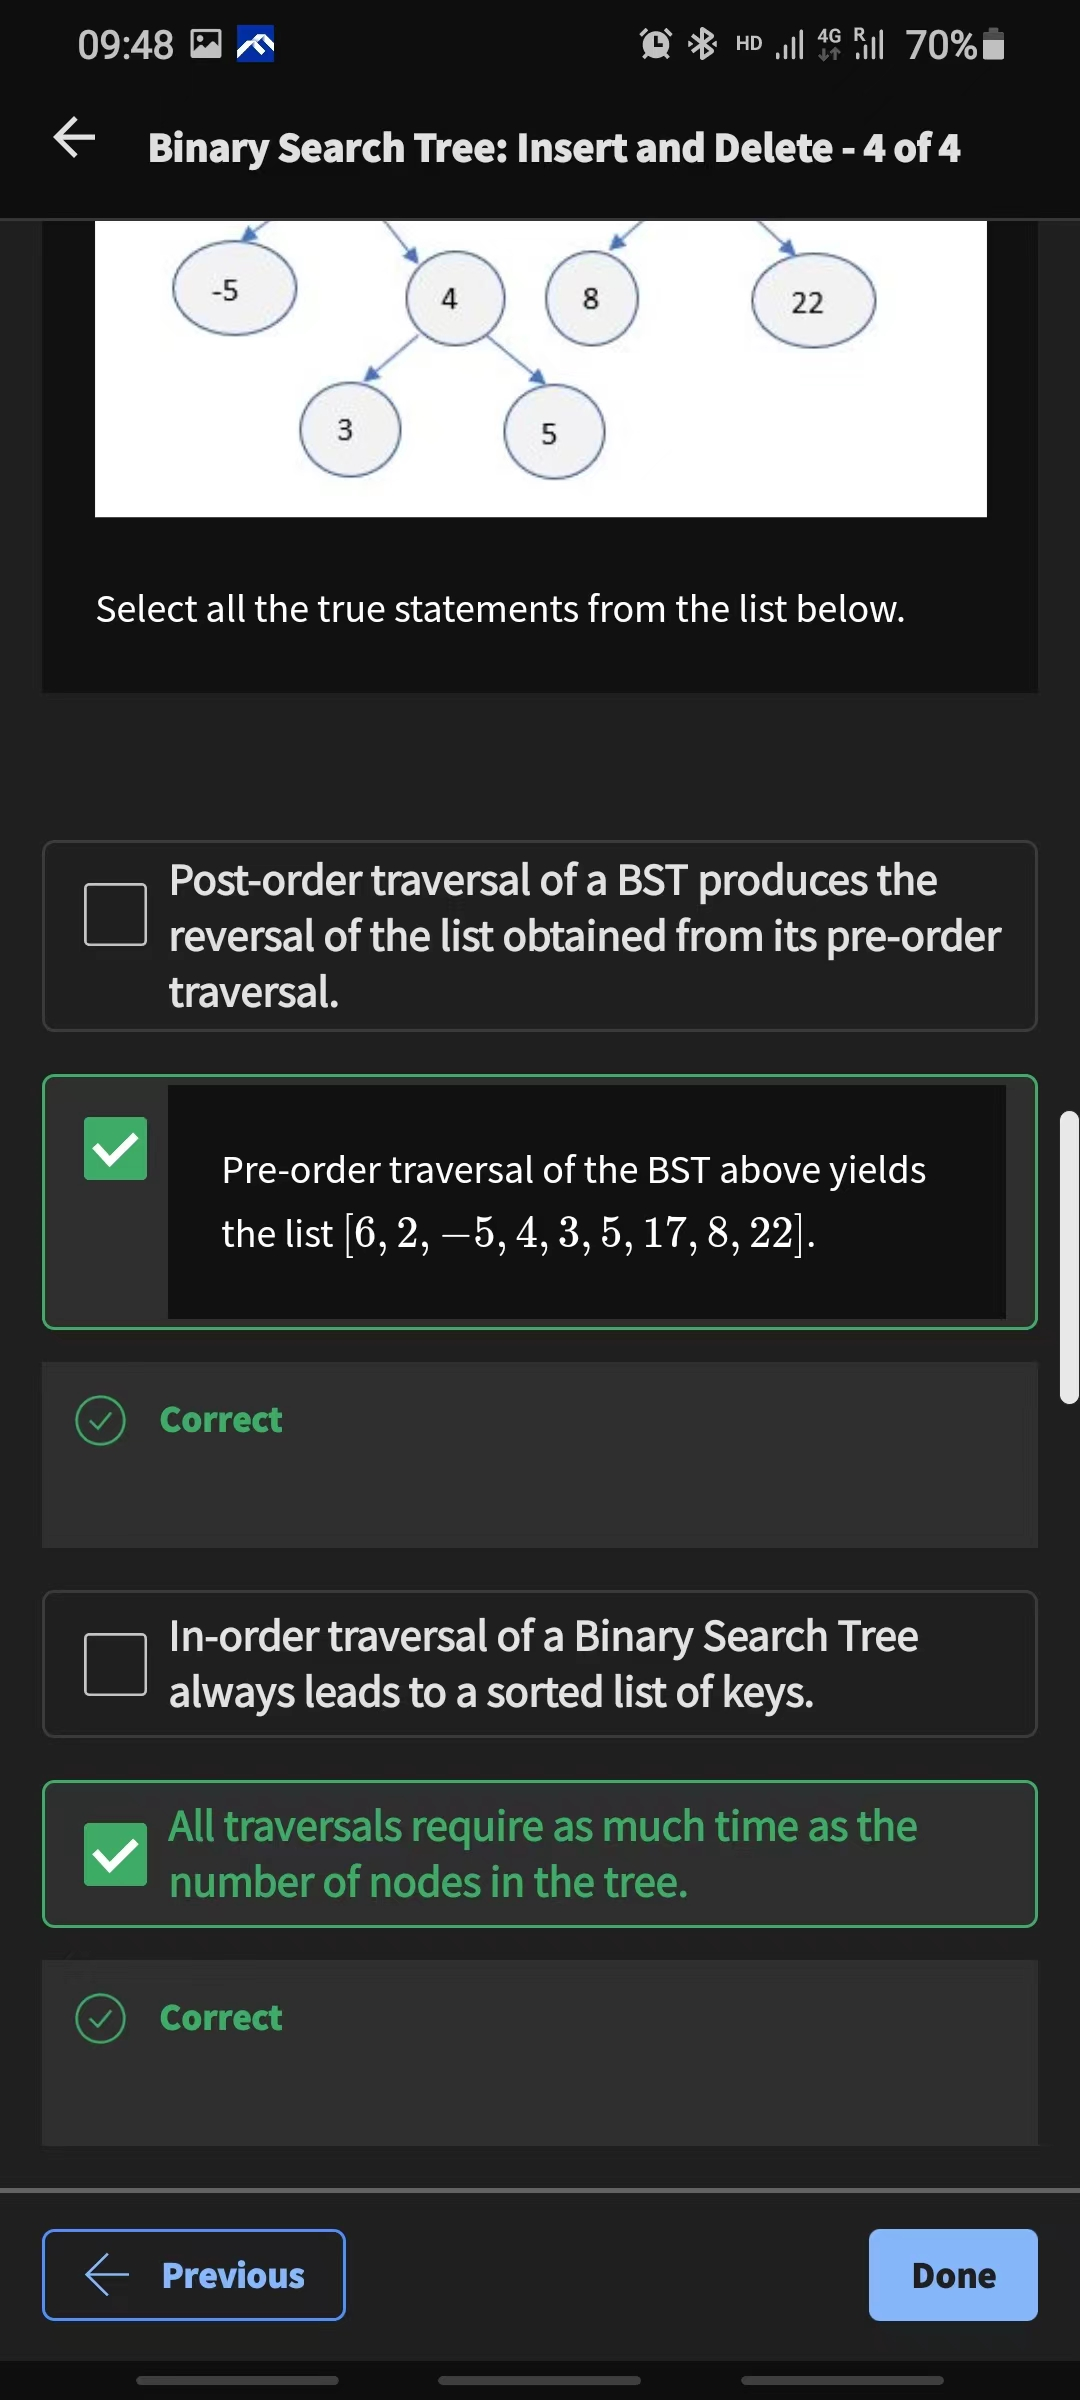
\includegraphics[width=0.45\textwidth]{bstinsertiondeletionquiz4-2.jpg}
    }
    \caption{Question 4}
    \label{fig:sidebyside}
\end{figure}





\section{Algorithms on Trees}


\subsection{Red-Black Trees Basics}

\paragraph{
    Normally the performance of a BST depends on its height or depth.\\
    If we have a bad (not well-balanced) binary search tree, the height of the tree will be $O(n)$.\\
    In this case, the performance of the tree will be the same as that of a linked list.\\
    If it's balanced, the running time will be as good as $O(\log(n))$. This is not good enough.\\
    What we need is self-balancing BSTs.\\
    Here are some different types of self-balancing BSTs.\\
}

\begin{figure}[H]
    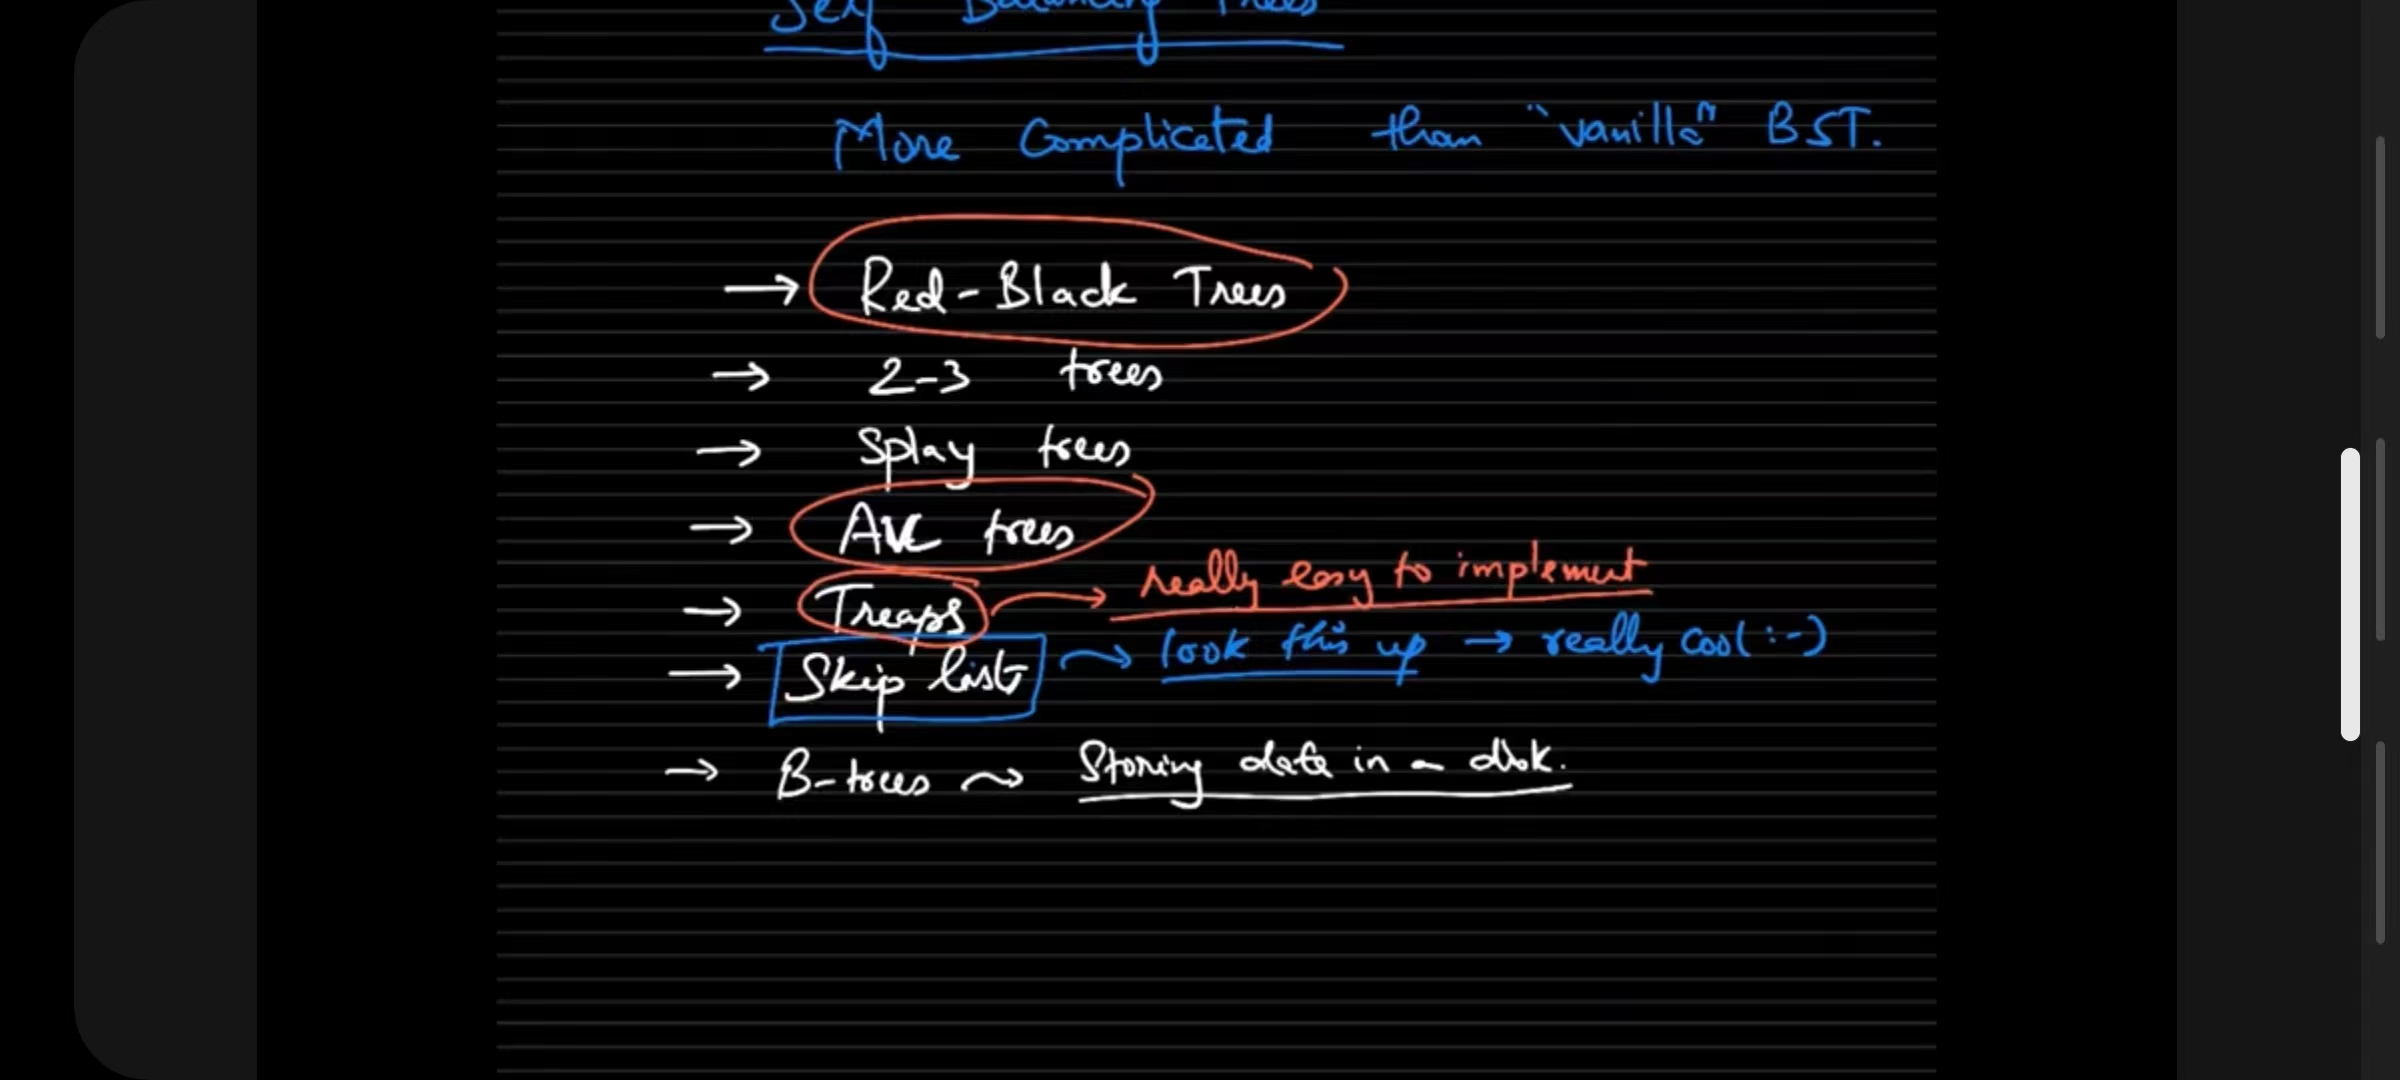
\includegraphics[width=\textwidth]{differenttypesofbst.jpg}
\end{figure}

\paragraph{
    Red-black trees are a type of self-balancing binary search tree.\\
    They are named after their property of having red and black nodes.\\
    The red-black tree has the following properties:\\
    1. Every node is either red or black.\\
    2. The root node is always black.\\
    3. Every leaf node is black.\\
    4. If a red node has children, the children must be black.\\
    5. Every path from a node to its descendant NIL nodes must have the same number of black nodes.\\
    The height of a red-black tree is $O(\log(n))$.\\
    The red-black tree is a balanced binary search tree.\\
}

\begin{figure}[H]
    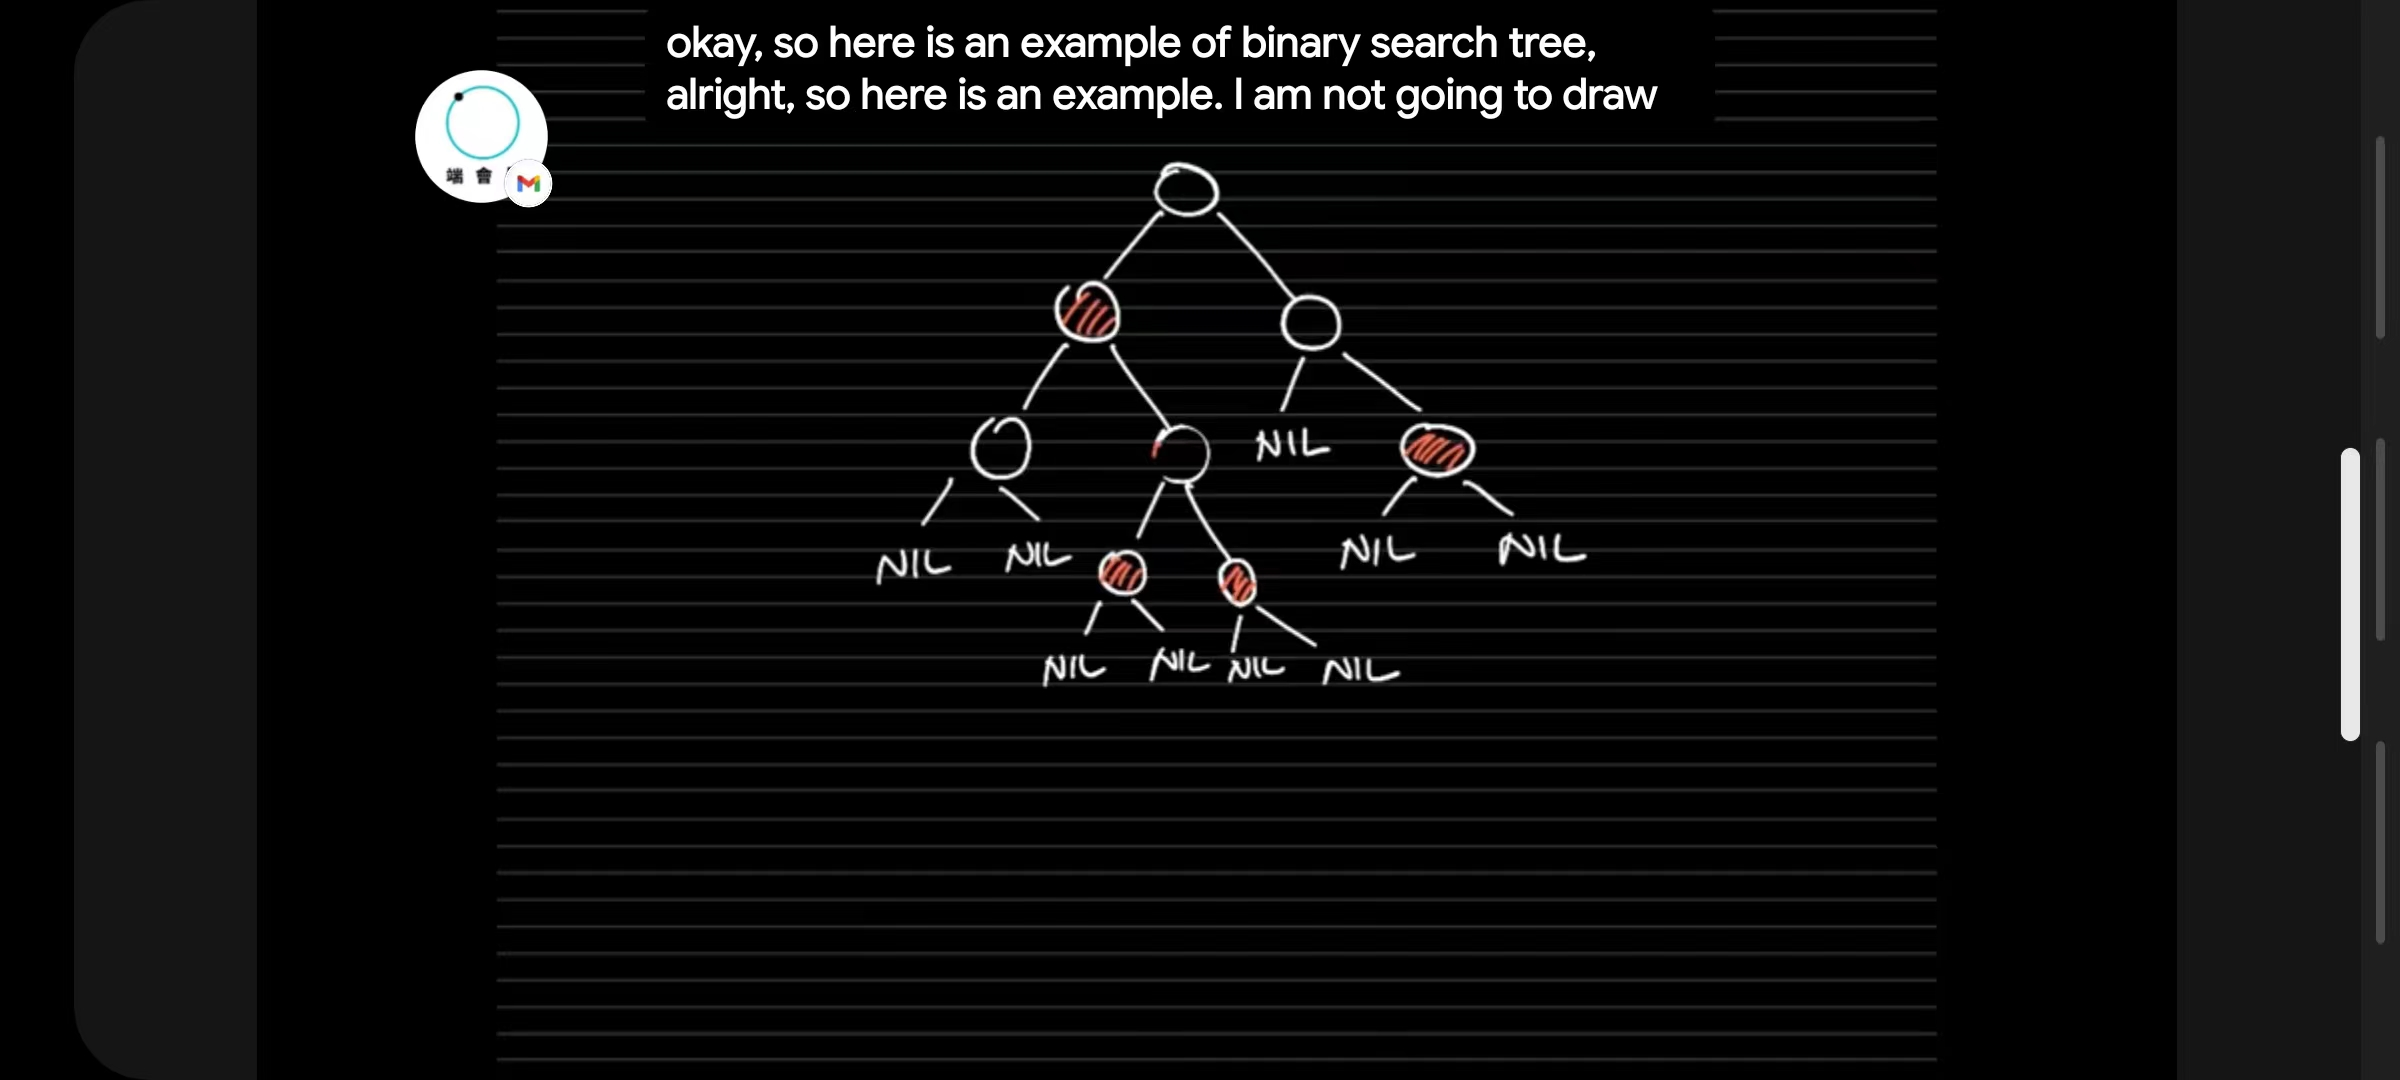
\includegraphics[width=\textwidth]{redblacktree.jpg}
\end{figure}

\begin{figure}[H]
    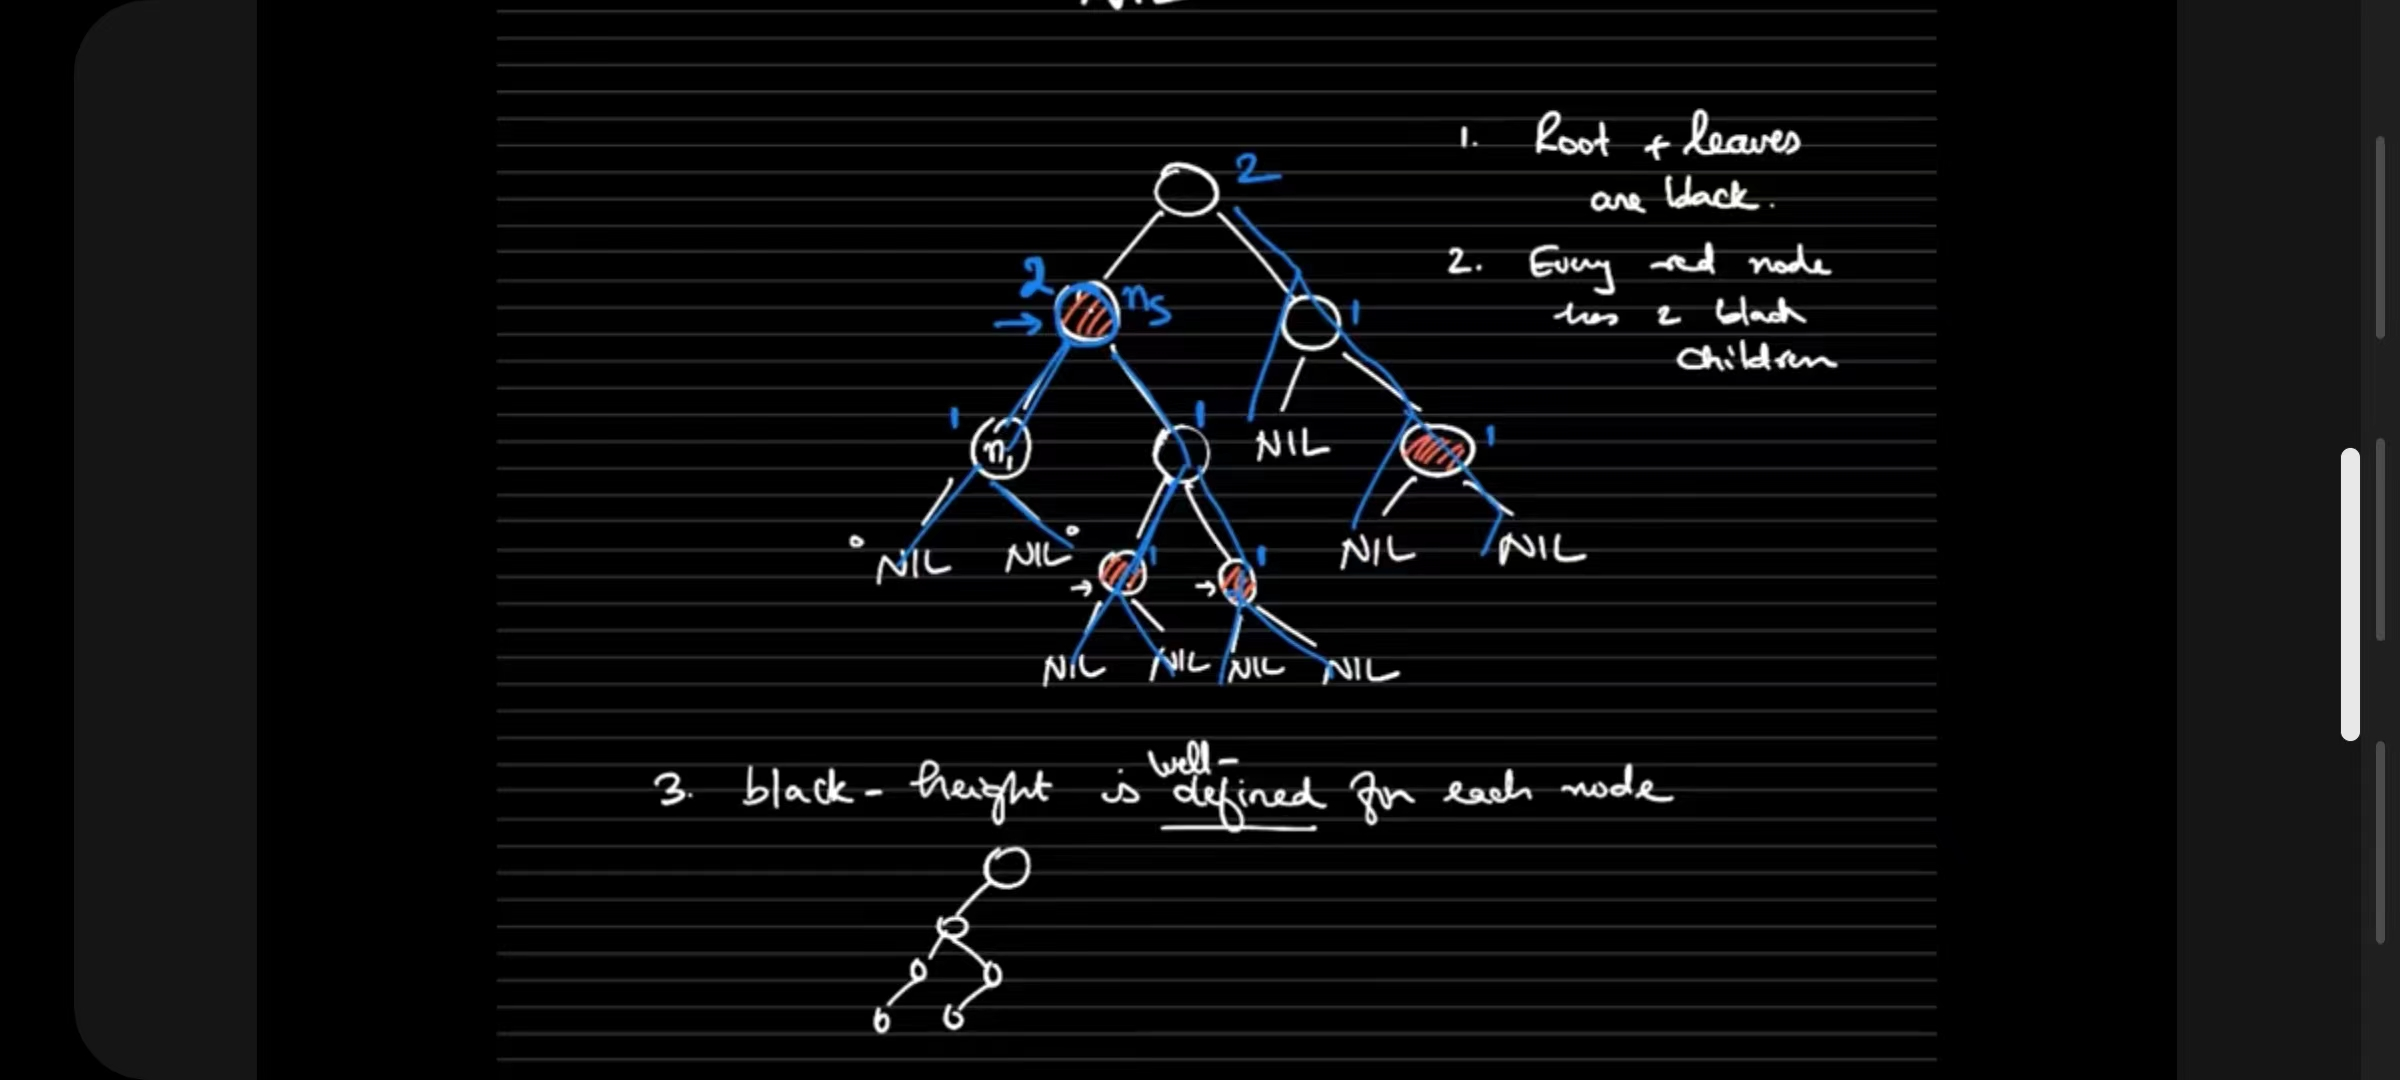
\includegraphics[width=\textwidth]{redblacktreesamenumberofblacknoderule.jpg}
\end{figure}

\paragraph{
    When counting the number of black nodes, we do not count the red nodes in between.\\
}

\begin{figure}[H]
    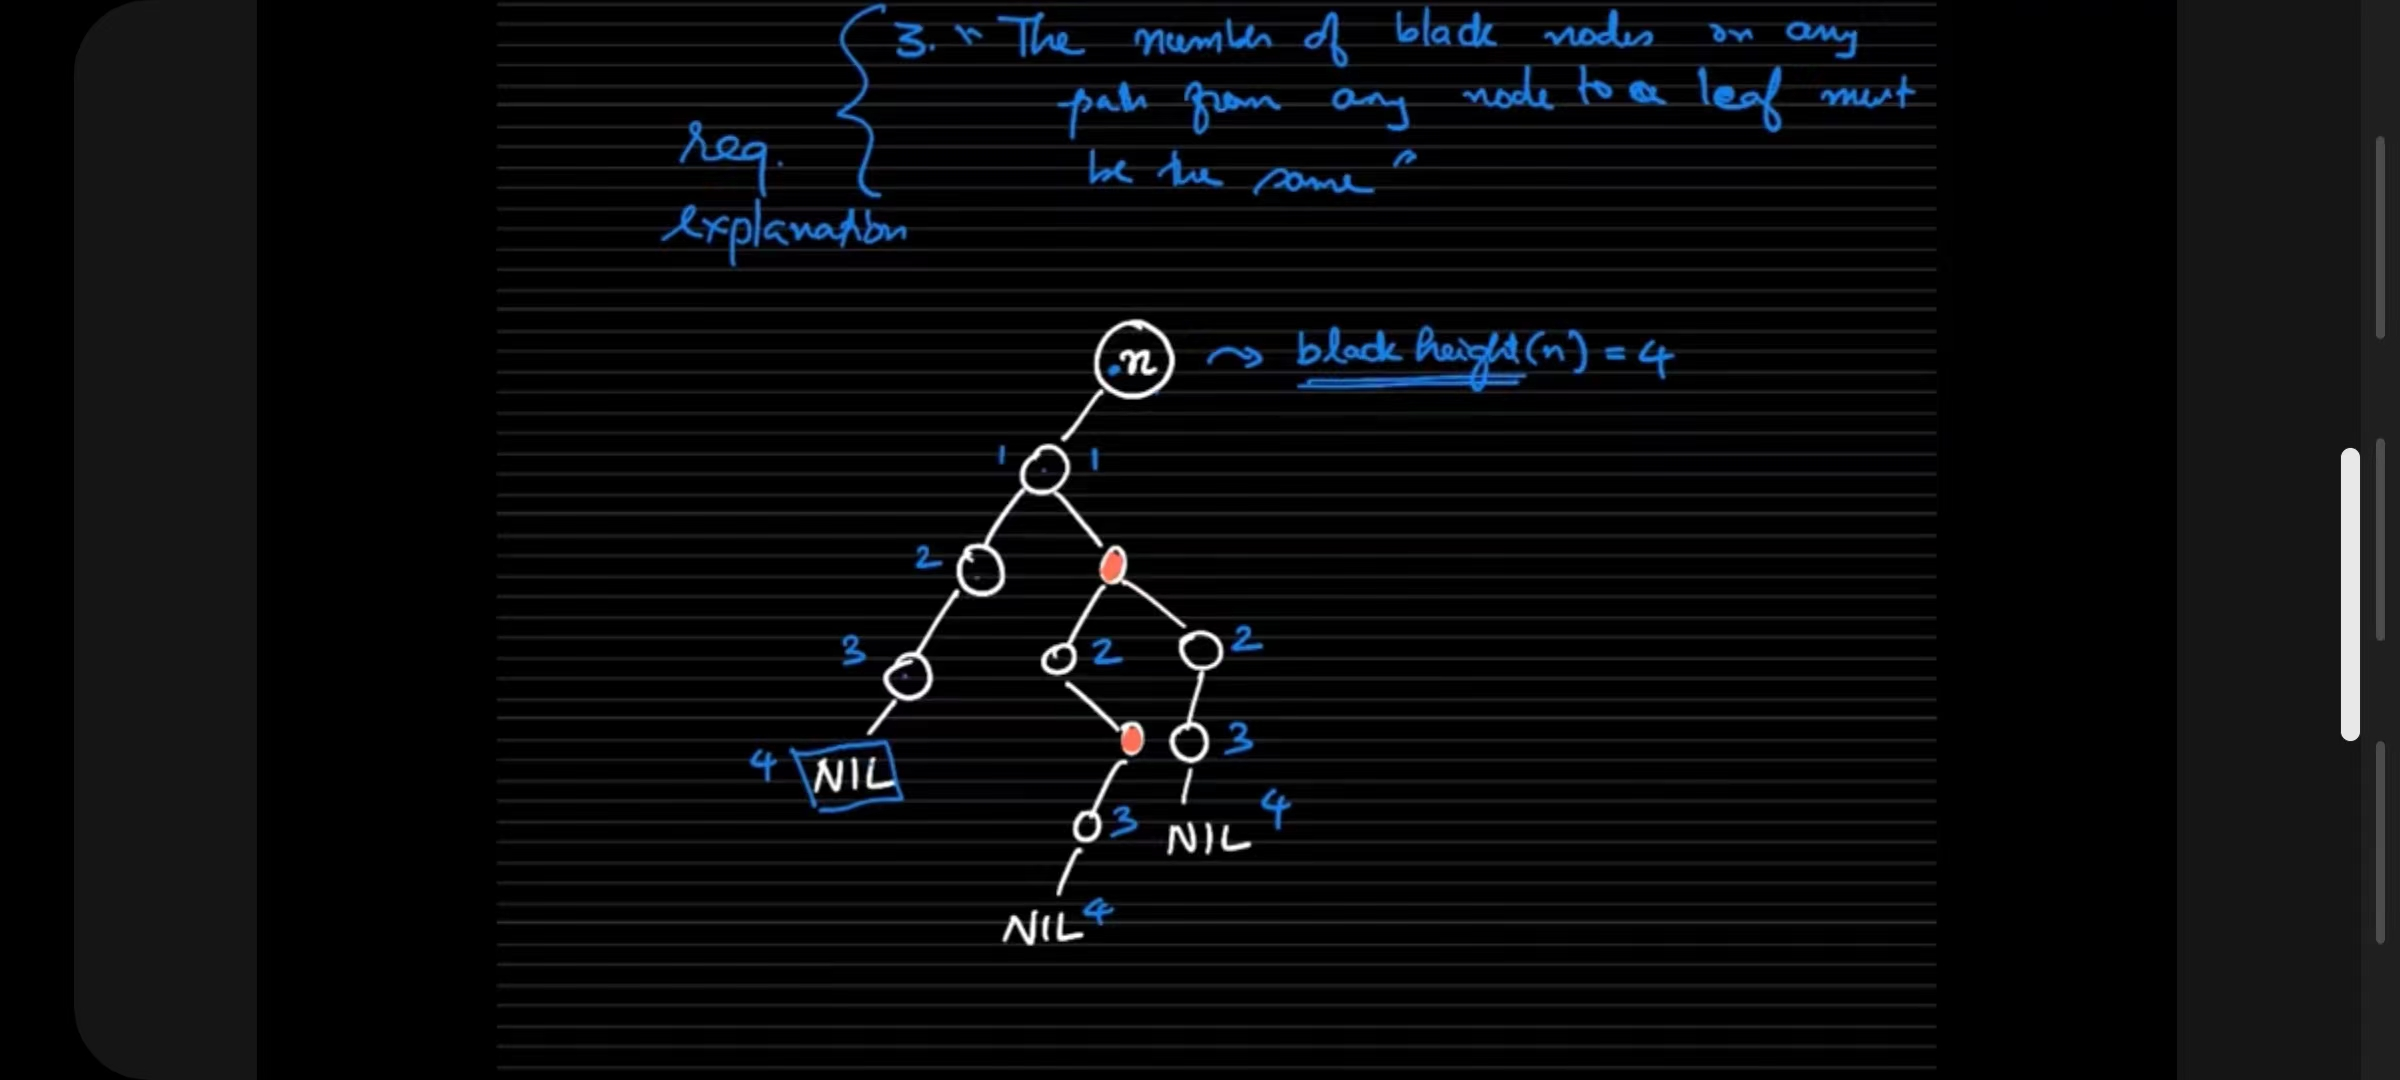
\includegraphics[width=\textwidth]{redblacktreeblackheight.jpg}
\end{figure}

\paragraph{
    Here is a question regarding red-black trees.\\
    We can come up with two scenarios for it.\\
}

\begin{figure}[H]
    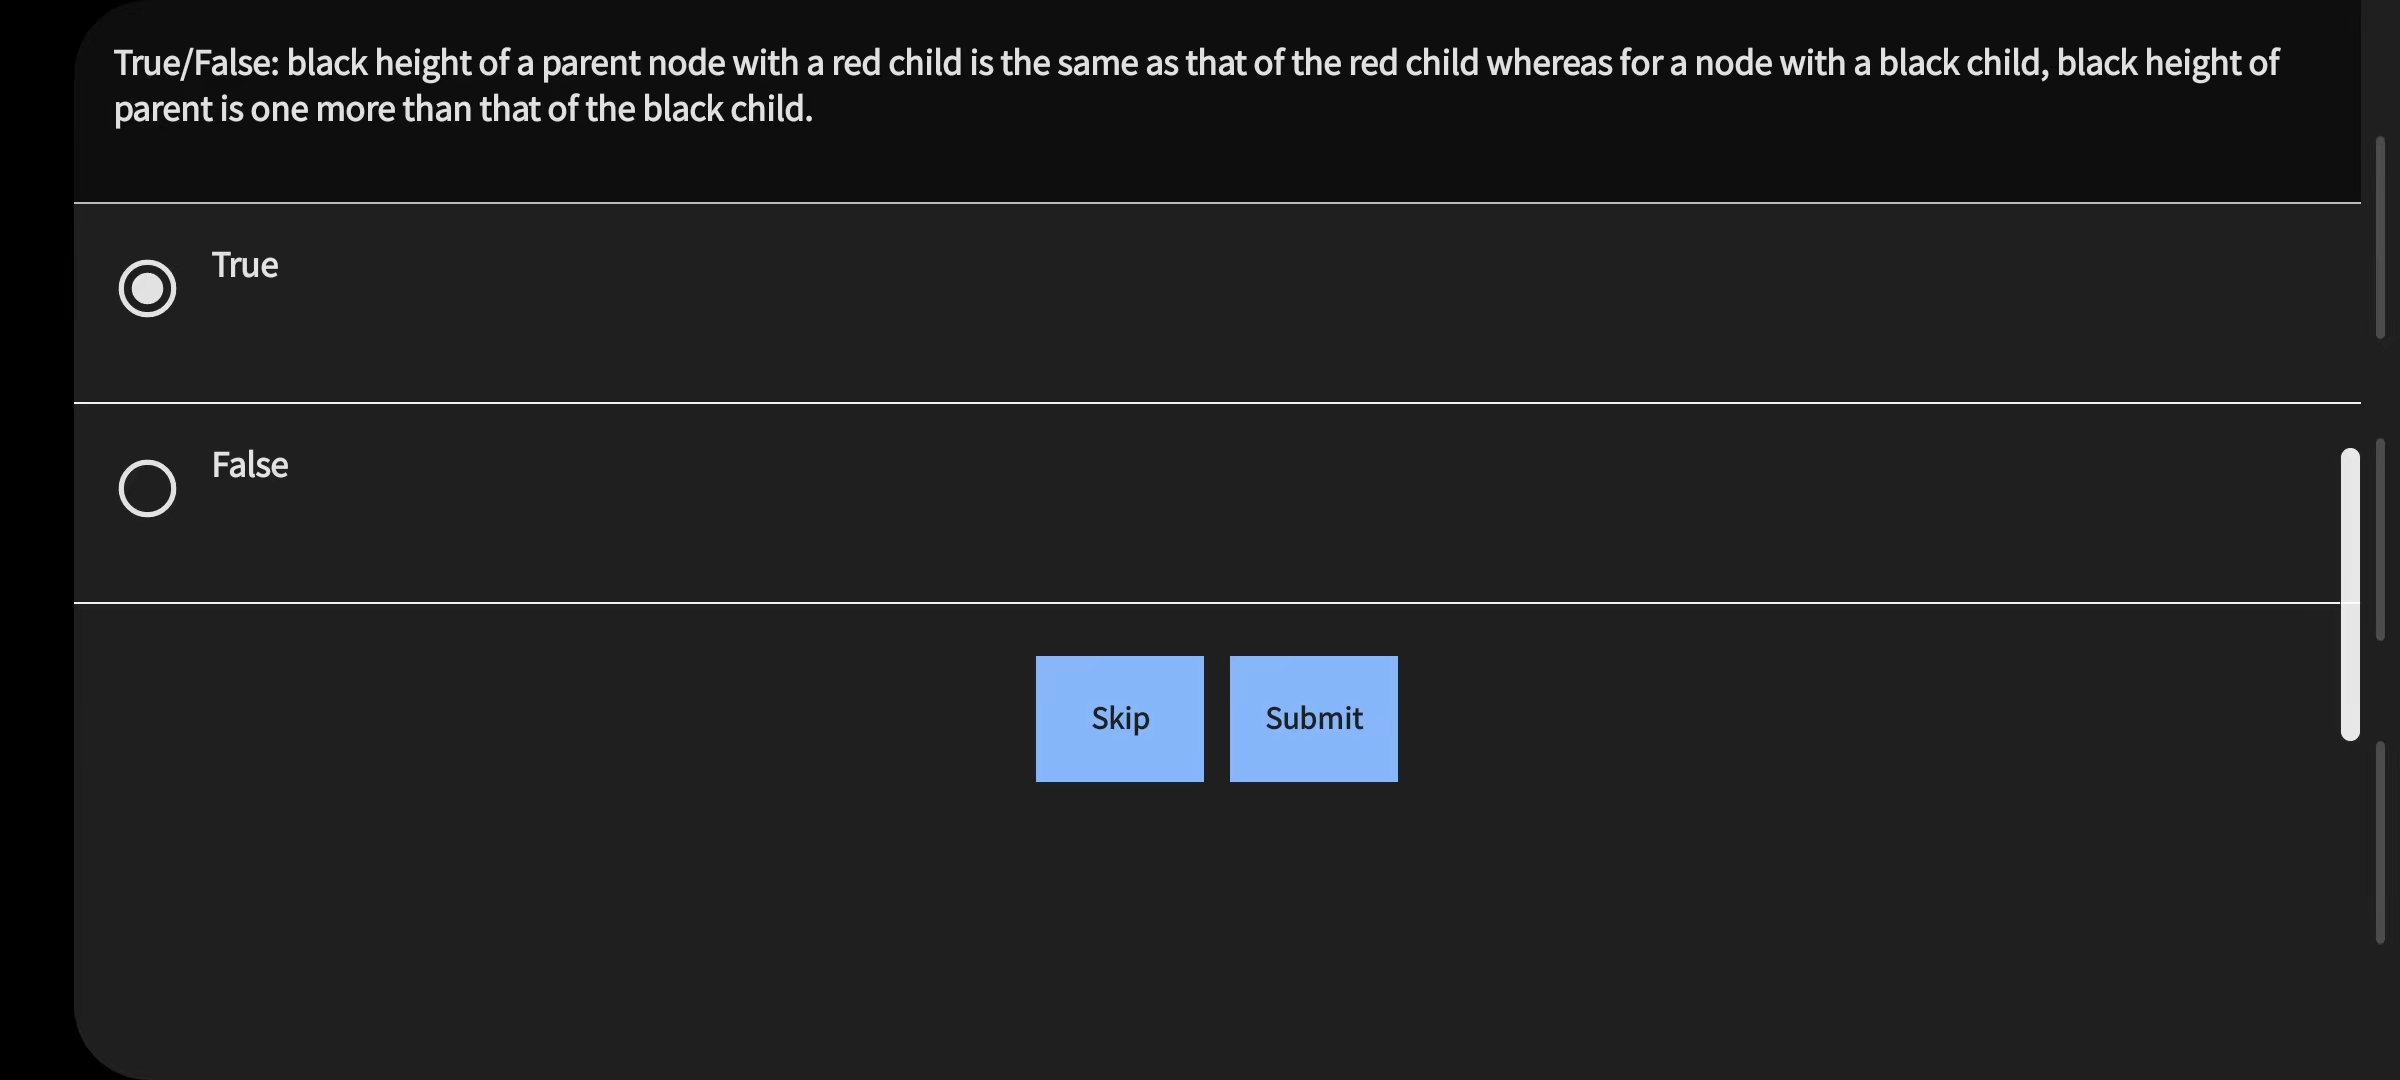
\includegraphics[width=\textwidth]{redblacktreequestion.jpg}
\end{figure}

\newpage
\begin{verbatim}
    Scenario 1:
    Parent node with RED child:
       B (parent node: height of 1)
         \
          red
         /   \
      NIL     NIL  (height of 1)
\end{verbatim}

\begin{verbatim}
    Scenario 2:
    Parent node with BLACK child:
       B (parent node: height of 2)
         \
           B (height of 1)
        /   \
       NIL  red
           /   \
        NIL     NIL  (height of 2)
\end{verbatim}    


\begin{figure}[H]
    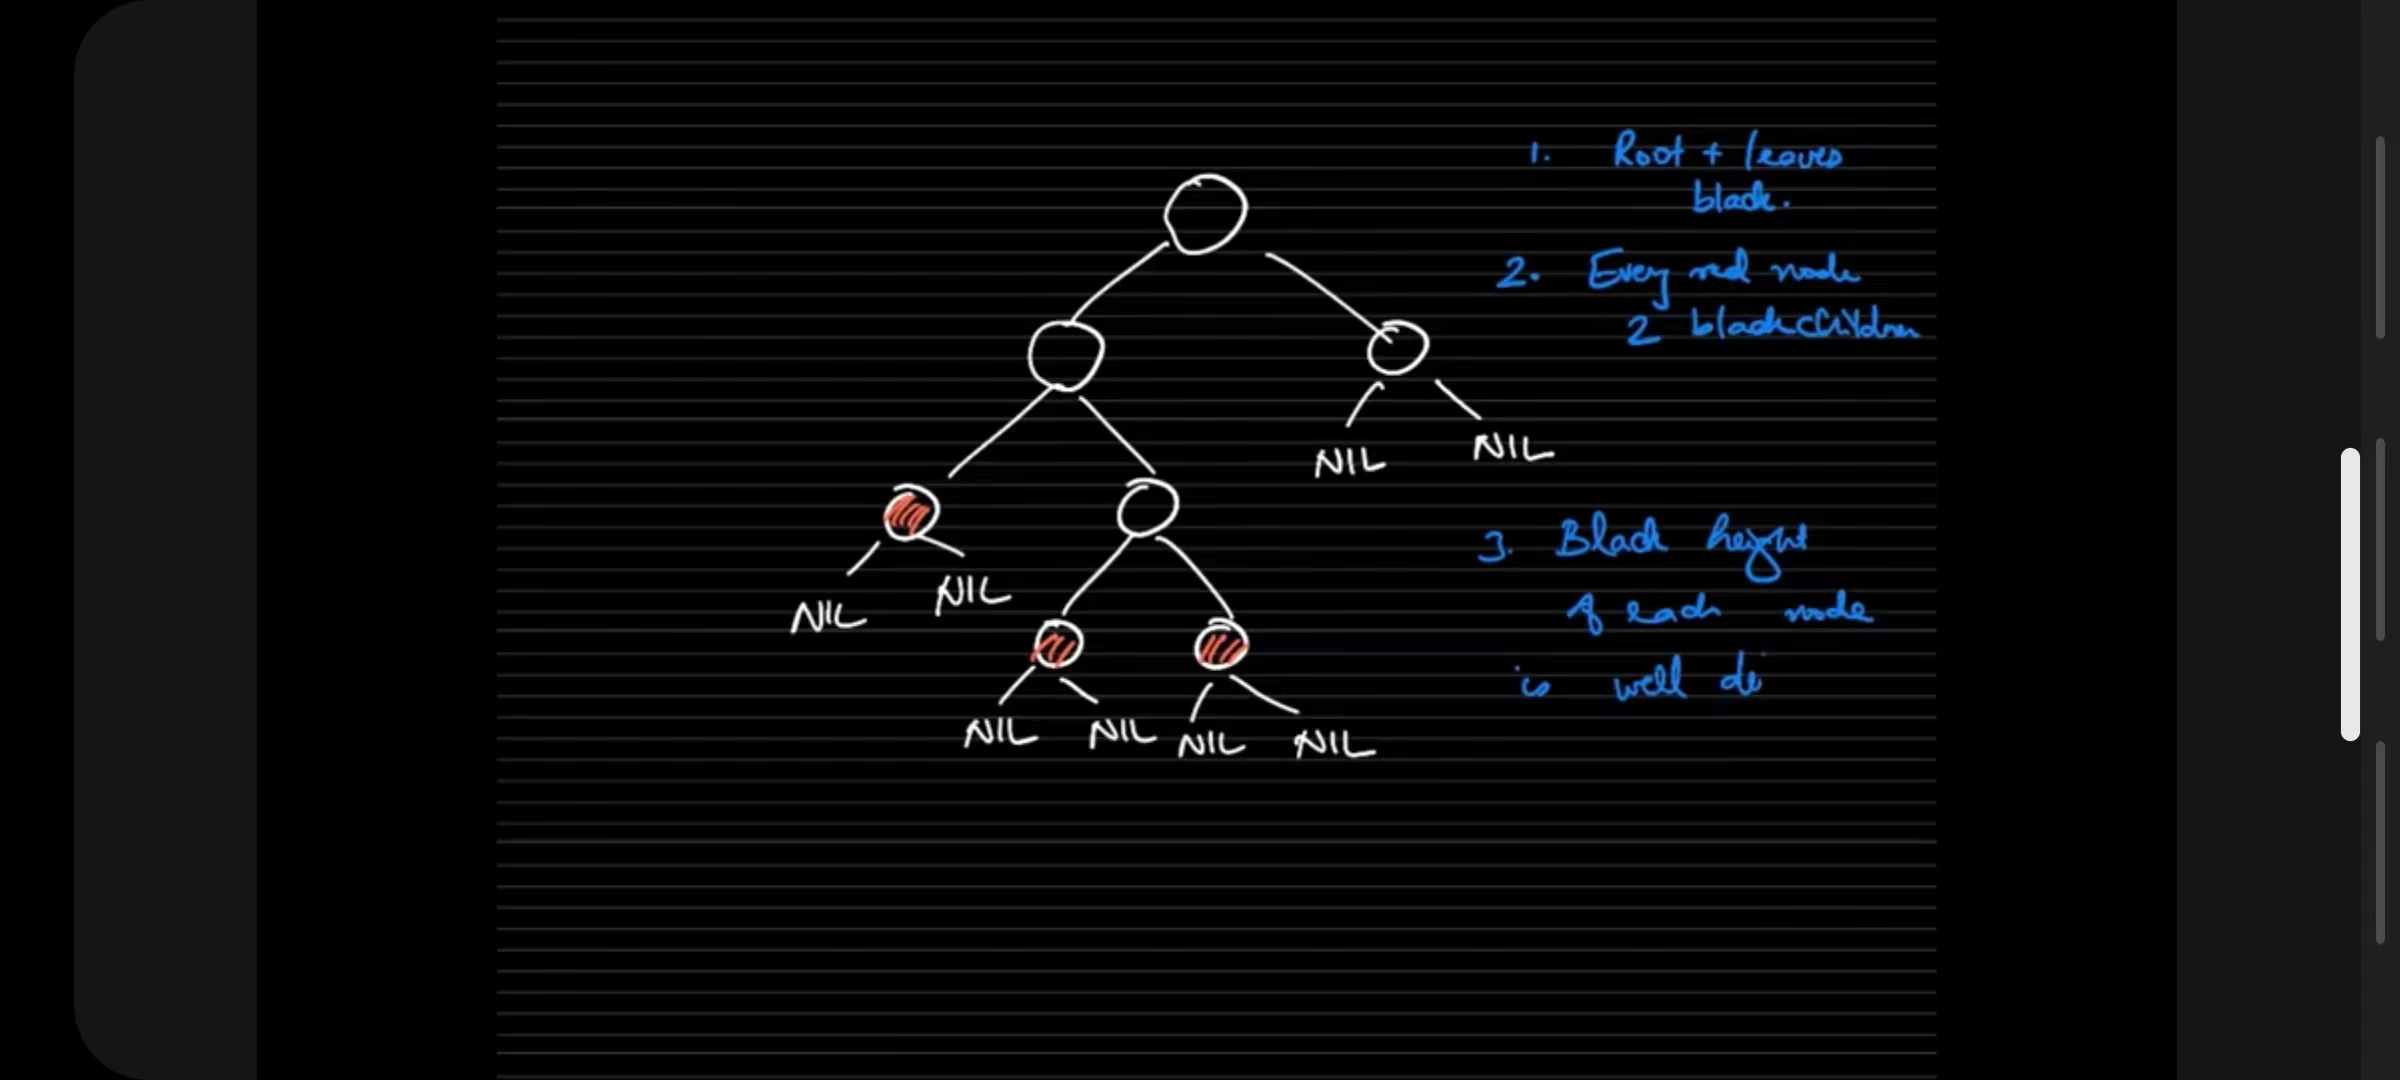
\includegraphics[width=\textwidth]{notredblacktree.jpg}
\end{figure}

\paragraph{
    As we can see, the tree in the figure is not a red-black tree.\\
    On the left corner, the height of the root node is 2, however, the height of the middle subtree is 3.\\
    For any red-black tree with $n$ nodes, the height $h$ must obey the following rule: \\
    $\log(n) \leq h \leq 2*\log(n)$.\\
    Here is another example of a unbalanced tree that cannot satisfy the red-black tree properties.\\
}

\begin{figure}[H]
    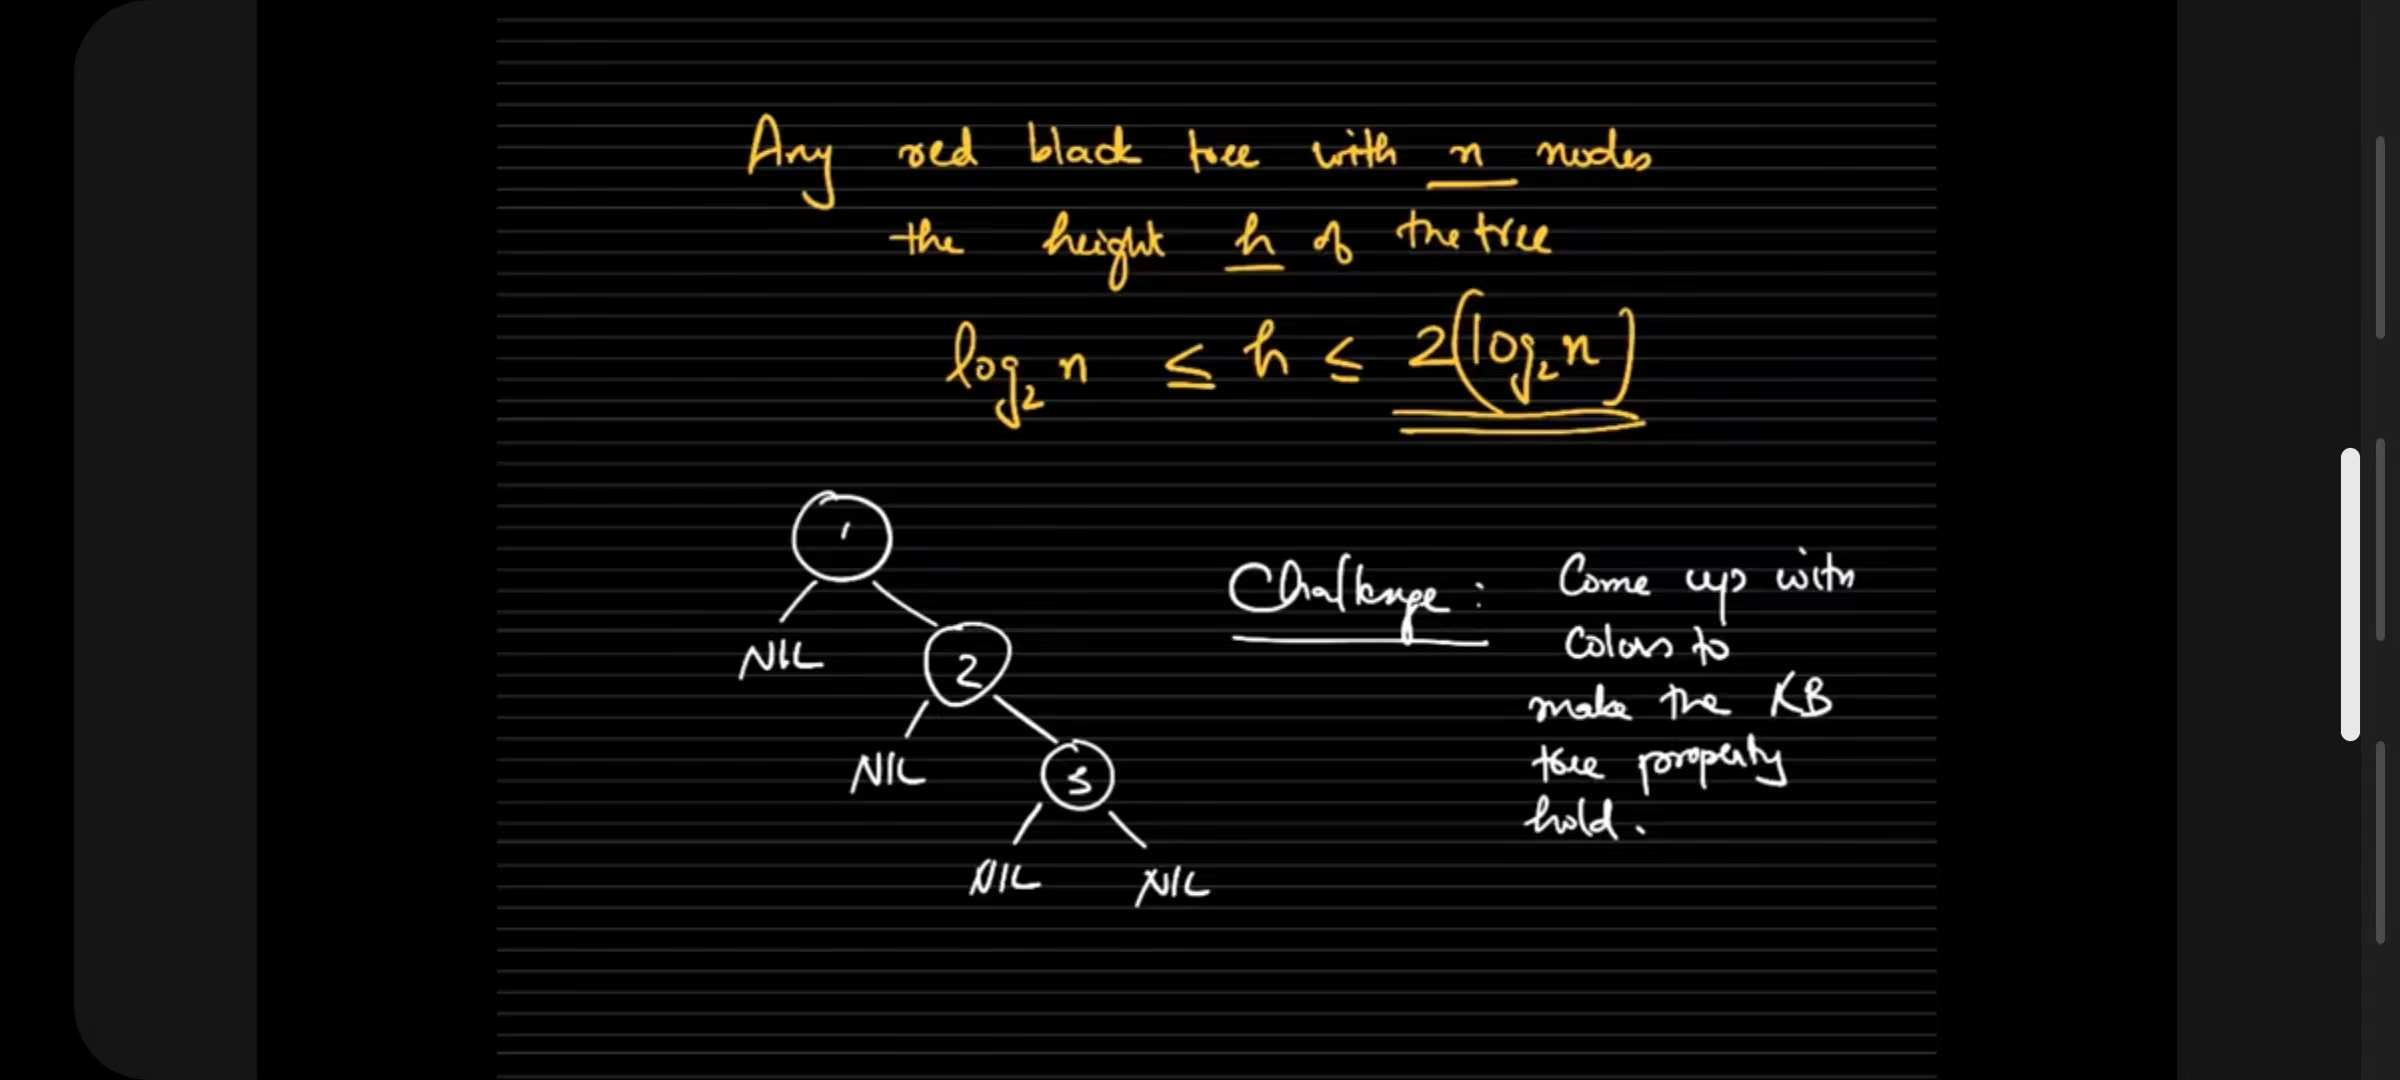
\includegraphics[width=\textwidth]{notbalancedtree.jpg}
\end{figure}


\paragraph{
    Now we can try to figure out how can we find a red-black tree.\\
    Suppose we have a $n$ node, $h$ height binary search tree.\\
    If it is a red-black tree, any path $l$ in the tree must be $h/2 < l < h$, since on any given path,
    at least half of the nodes must be black.\\
}

\begin{figure}[H]
    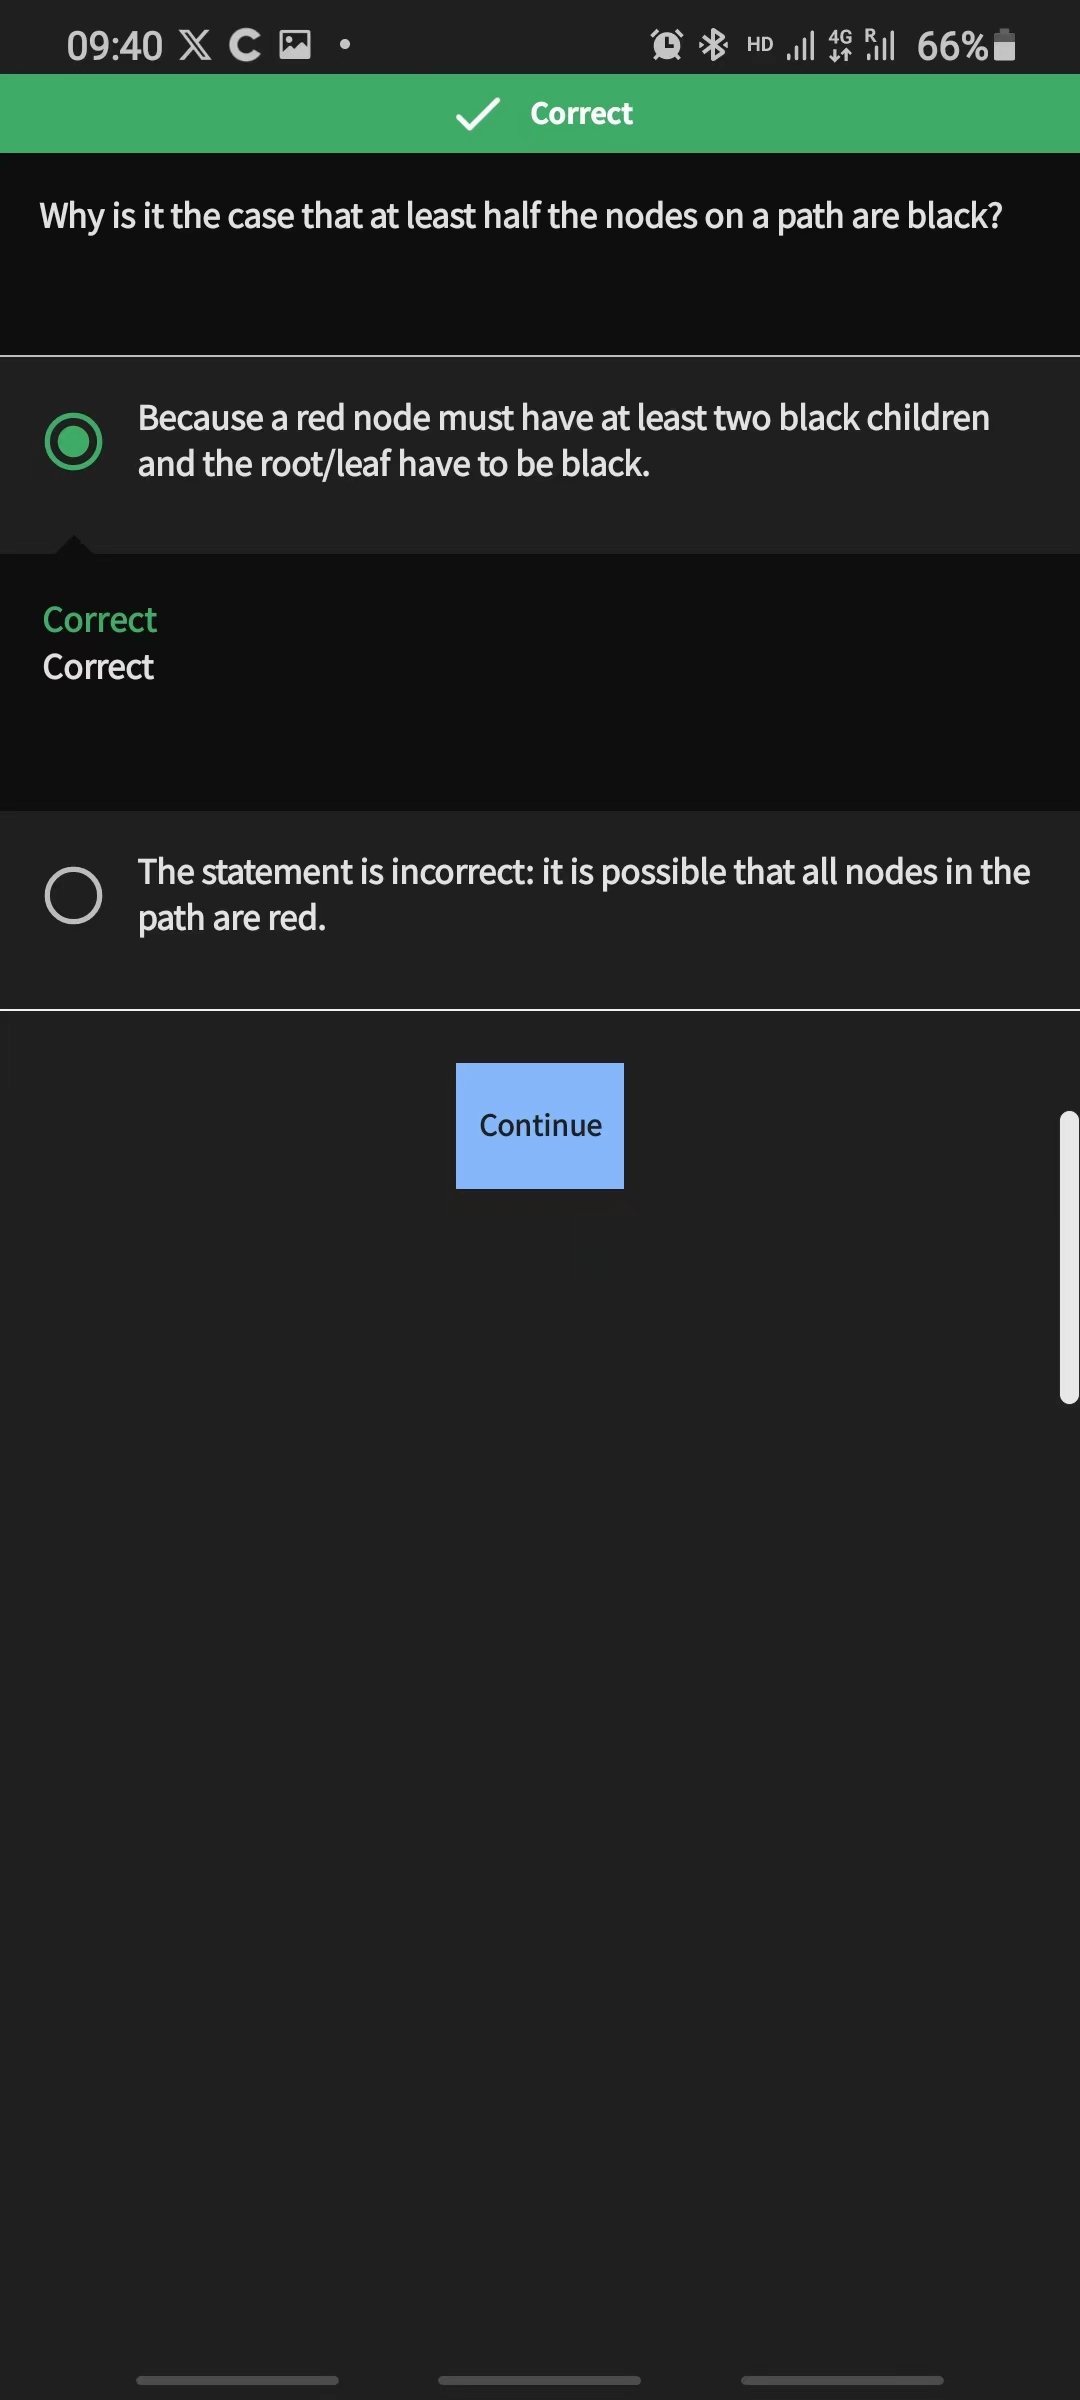
\includegraphics[width=\textwidth]{halfofthepathareblack.jpg}
\end{figure}

\begin{figure}[H]
    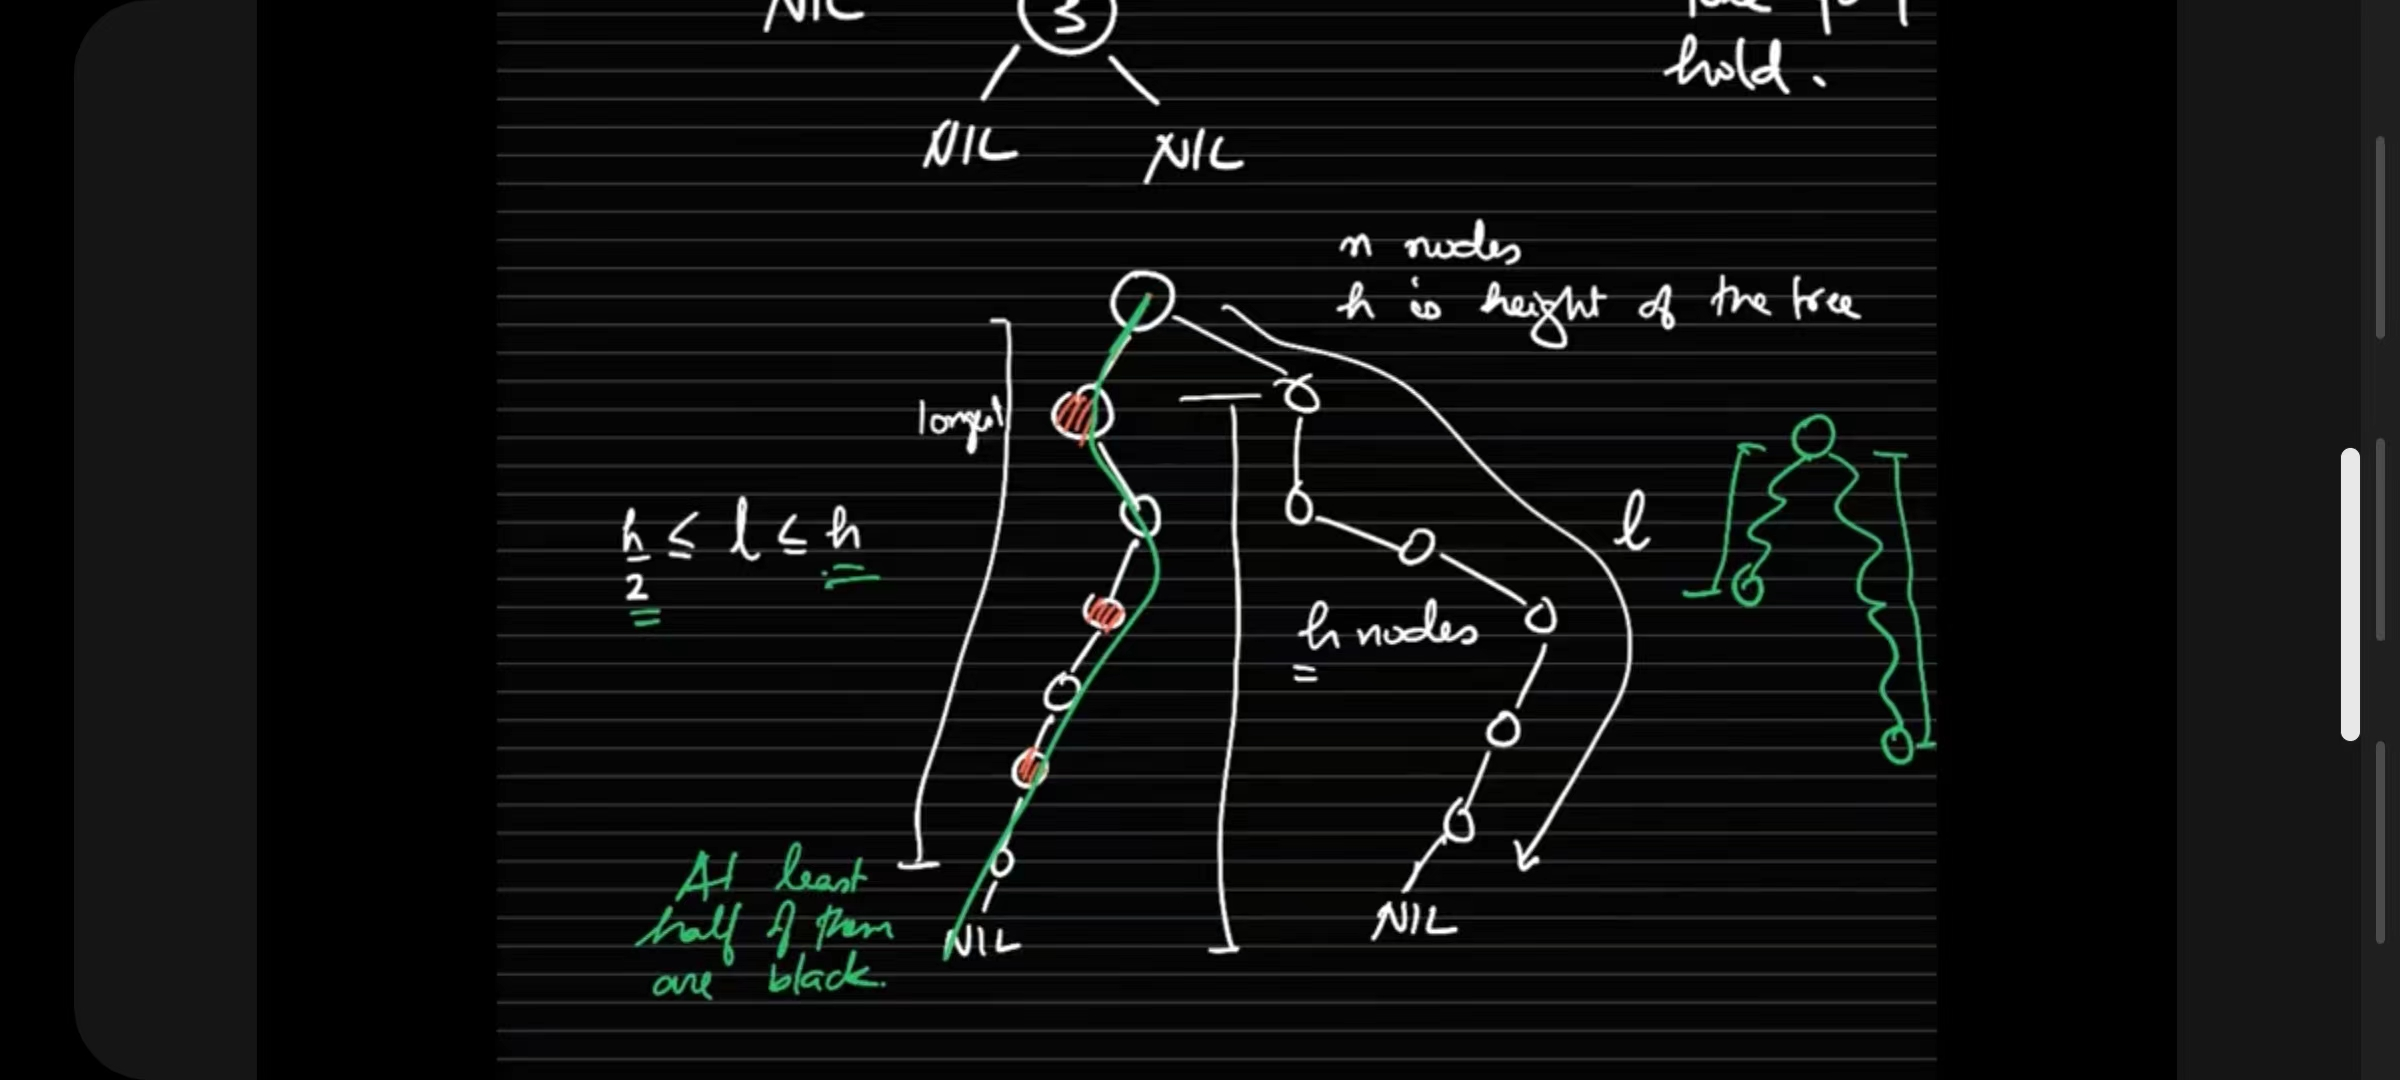
\includegraphics[width=\textwidth]{hrelated.jpg}
\end{figure}

\paragraph{
    Let's assume the black height of a specific node is $bh$. The subtree under that node will have a total node count $nc \geq 2^{bh} - 1$.\\
    This can be proved by induction, or we can also directly see the logic via such graph:\\
}

\begin{verbatim}
     N     1 node ---- 2^0
    / \    
   N   N   2 nodes --- 2^1
  / \ / \
N   N N  N 4 nodes --- 2^2
\end{verbatim}  

\paragraph{
    Since we have the property that any path $l \geq h/2$, we can say that $nc \geq 2^{bh} - 1 \geq 2^{h/2} - 1$.\\
    Then we can conclude that $h \leq 2*\log(n+1)$.\\
}

\begin{figure}[H]
    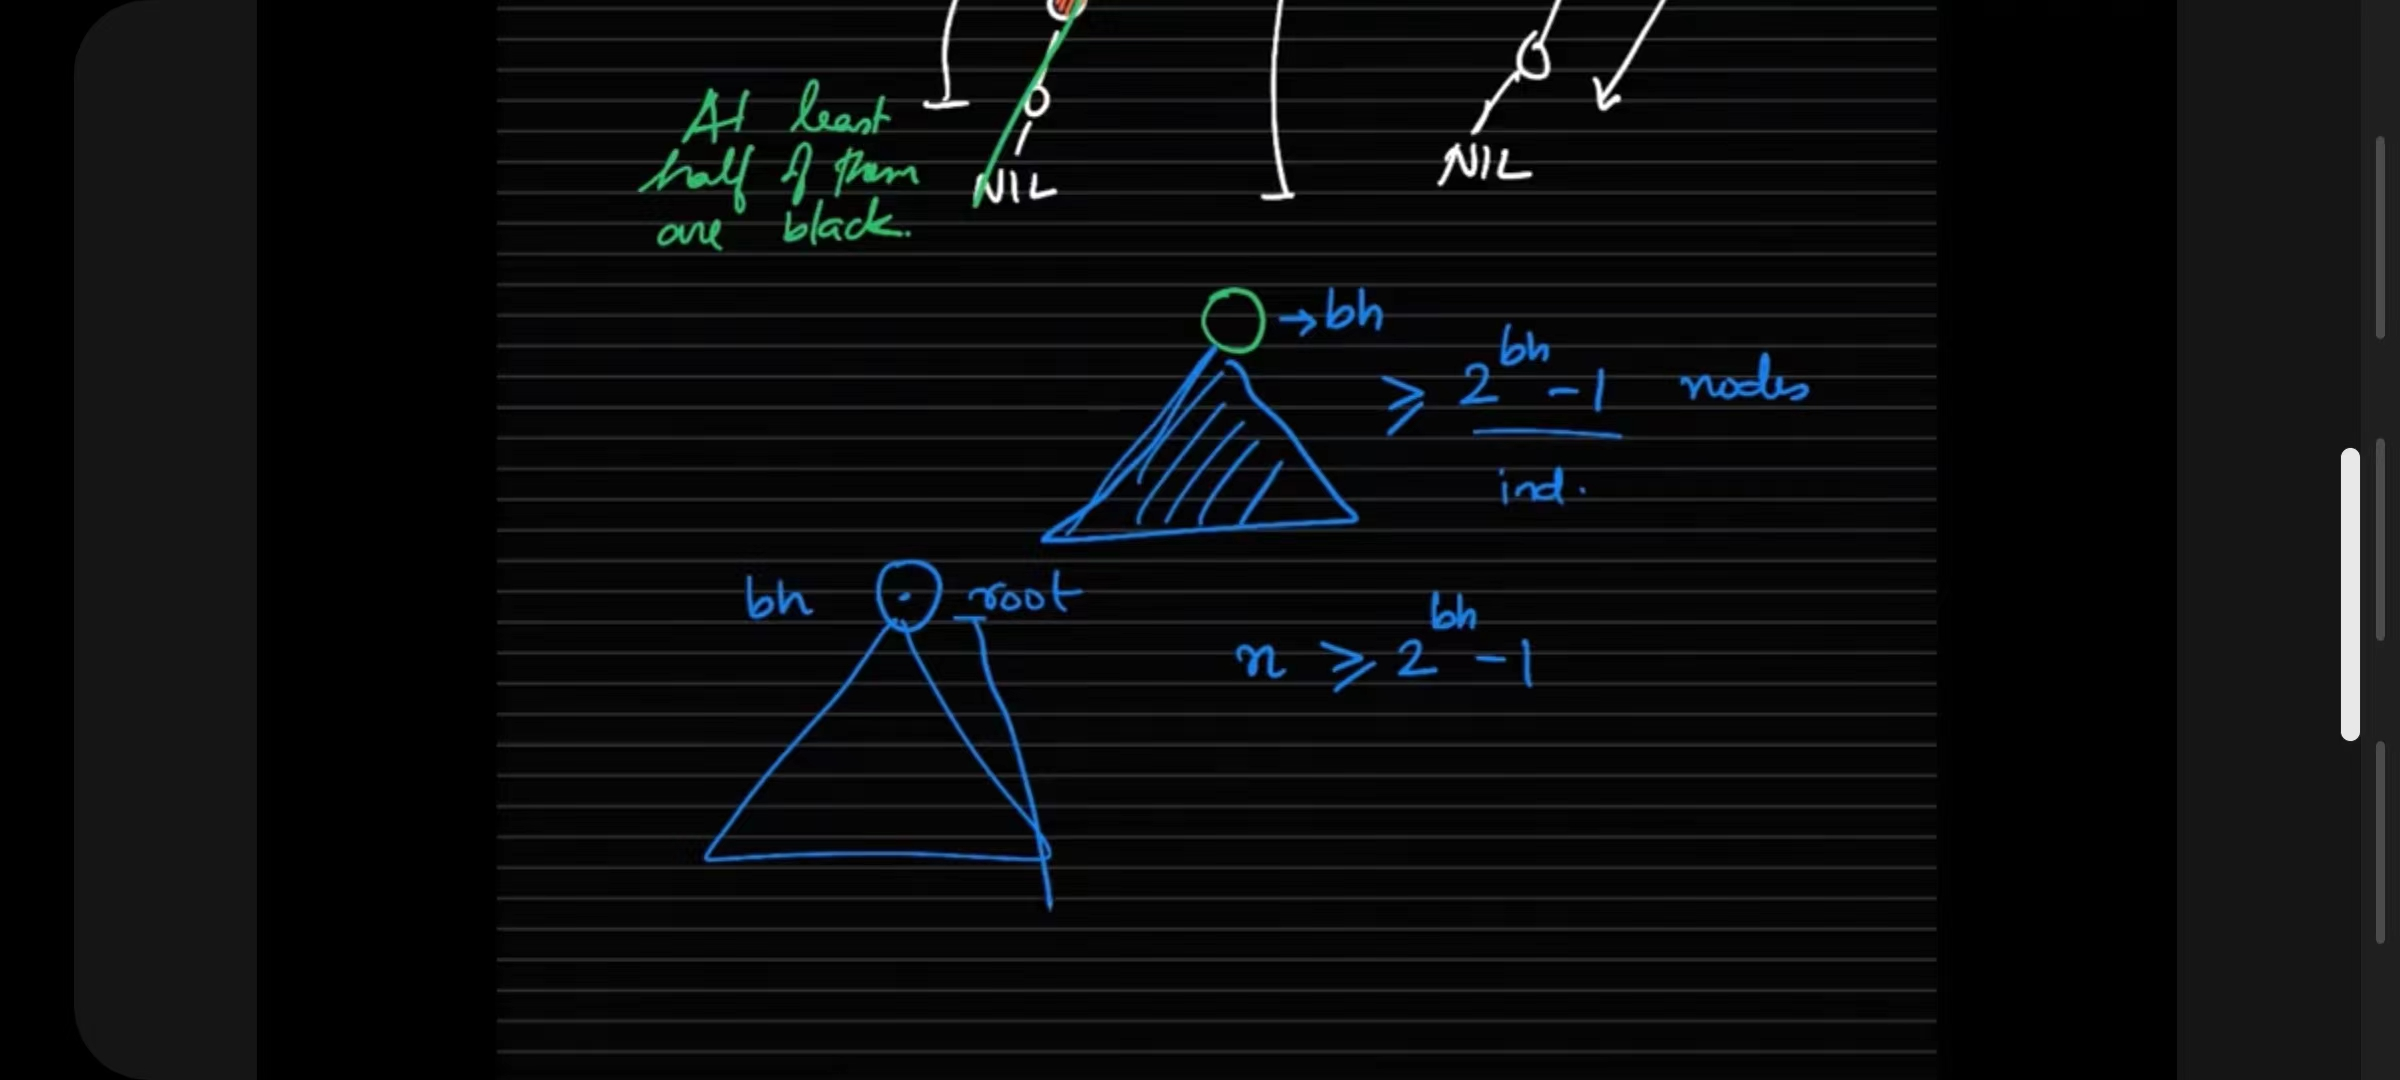
\includegraphics[width=\textwidth]{bhrelated.jpg}
\end{figure}

\subsubsection{RBT Quiz}


\begin{figure}[H]
    \centering
    \subfigure{
        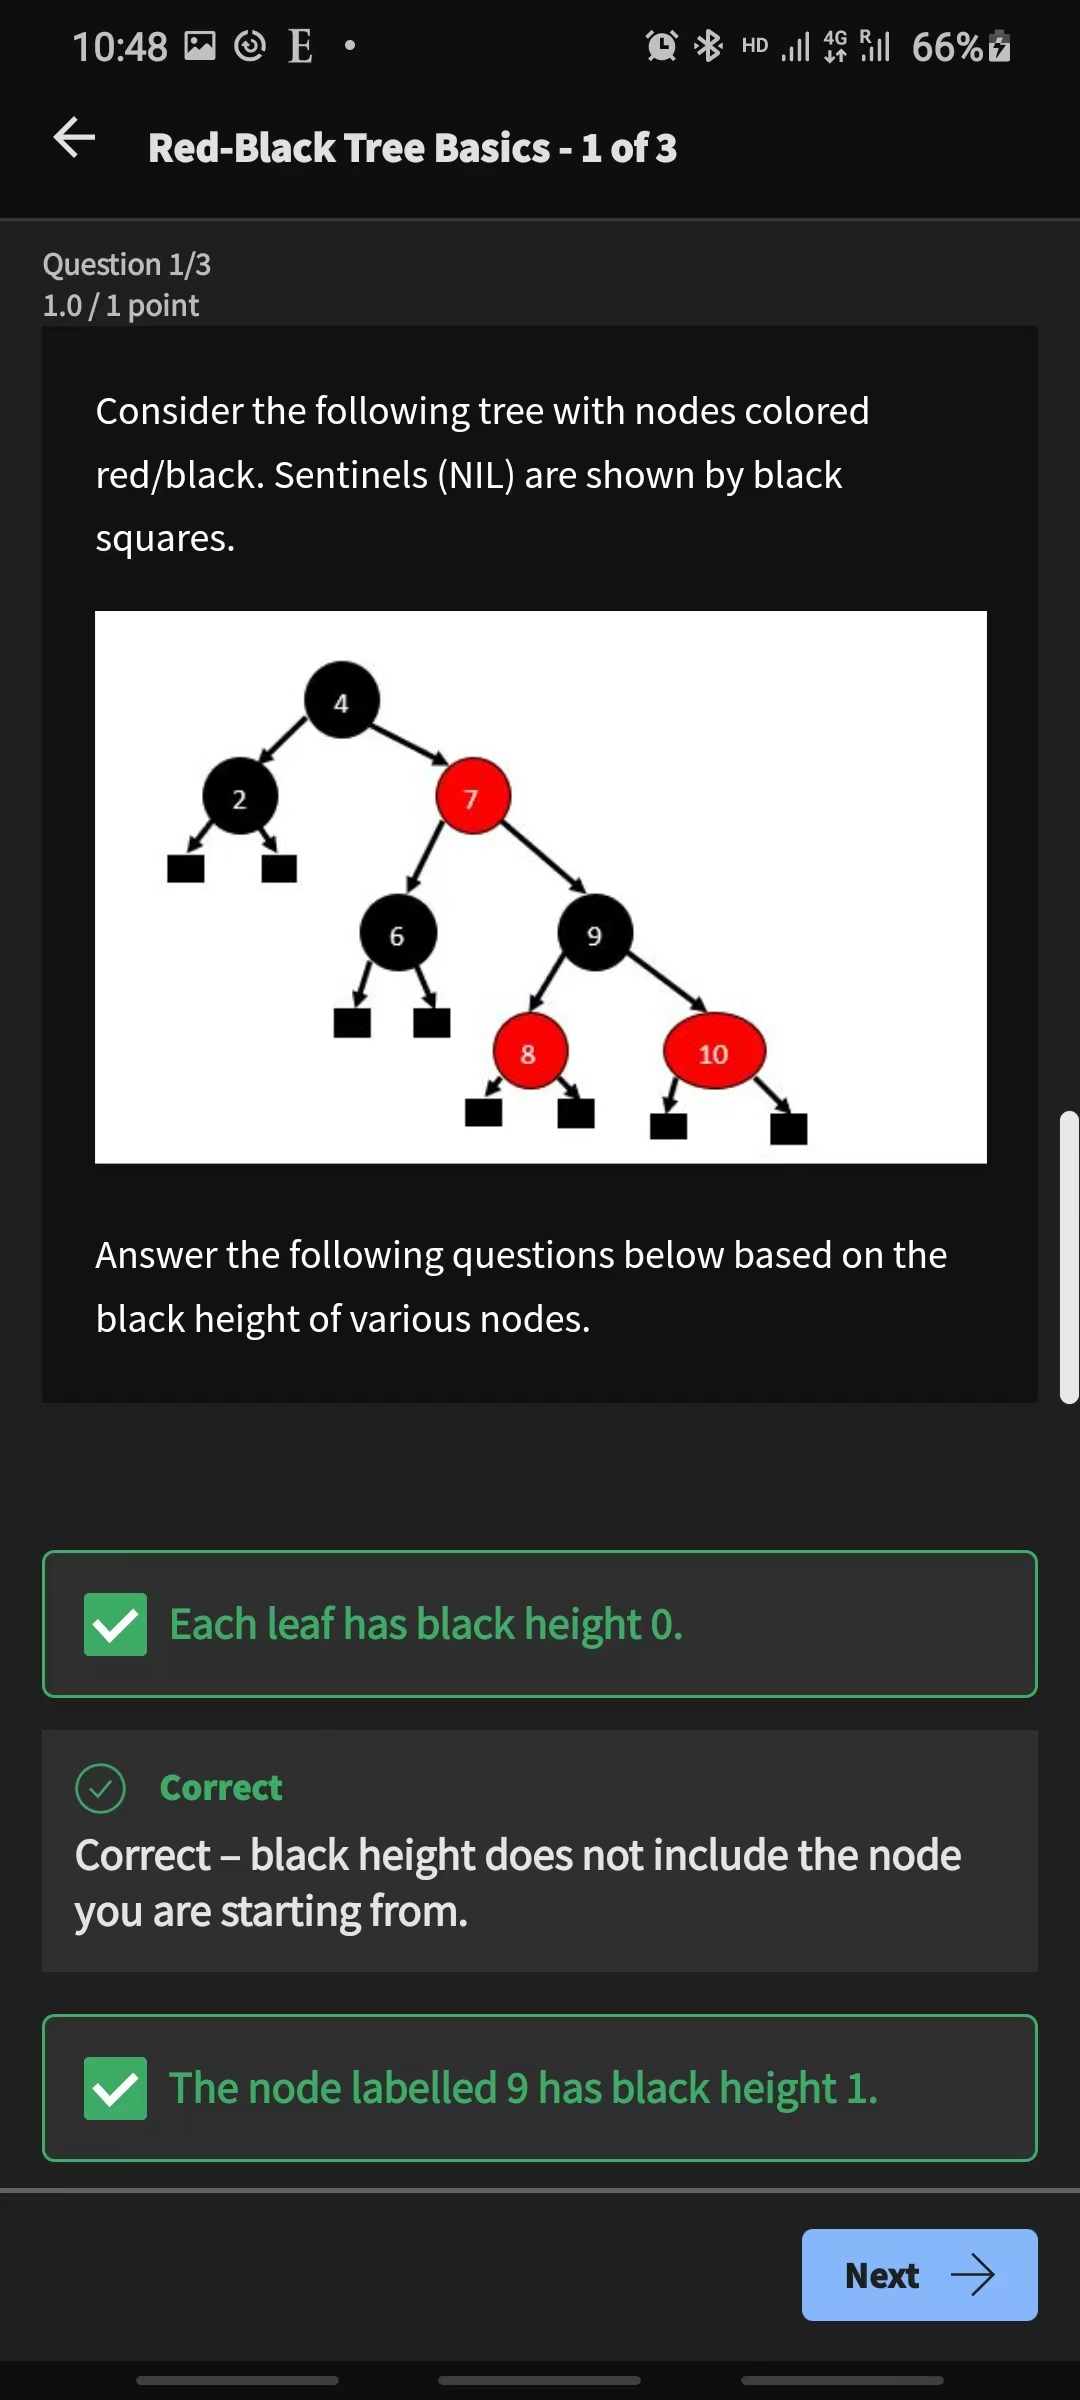
\includegraphics[width=0.45\textwidth]{rbtquiz01.jpg}
    }
    \subfigure{
        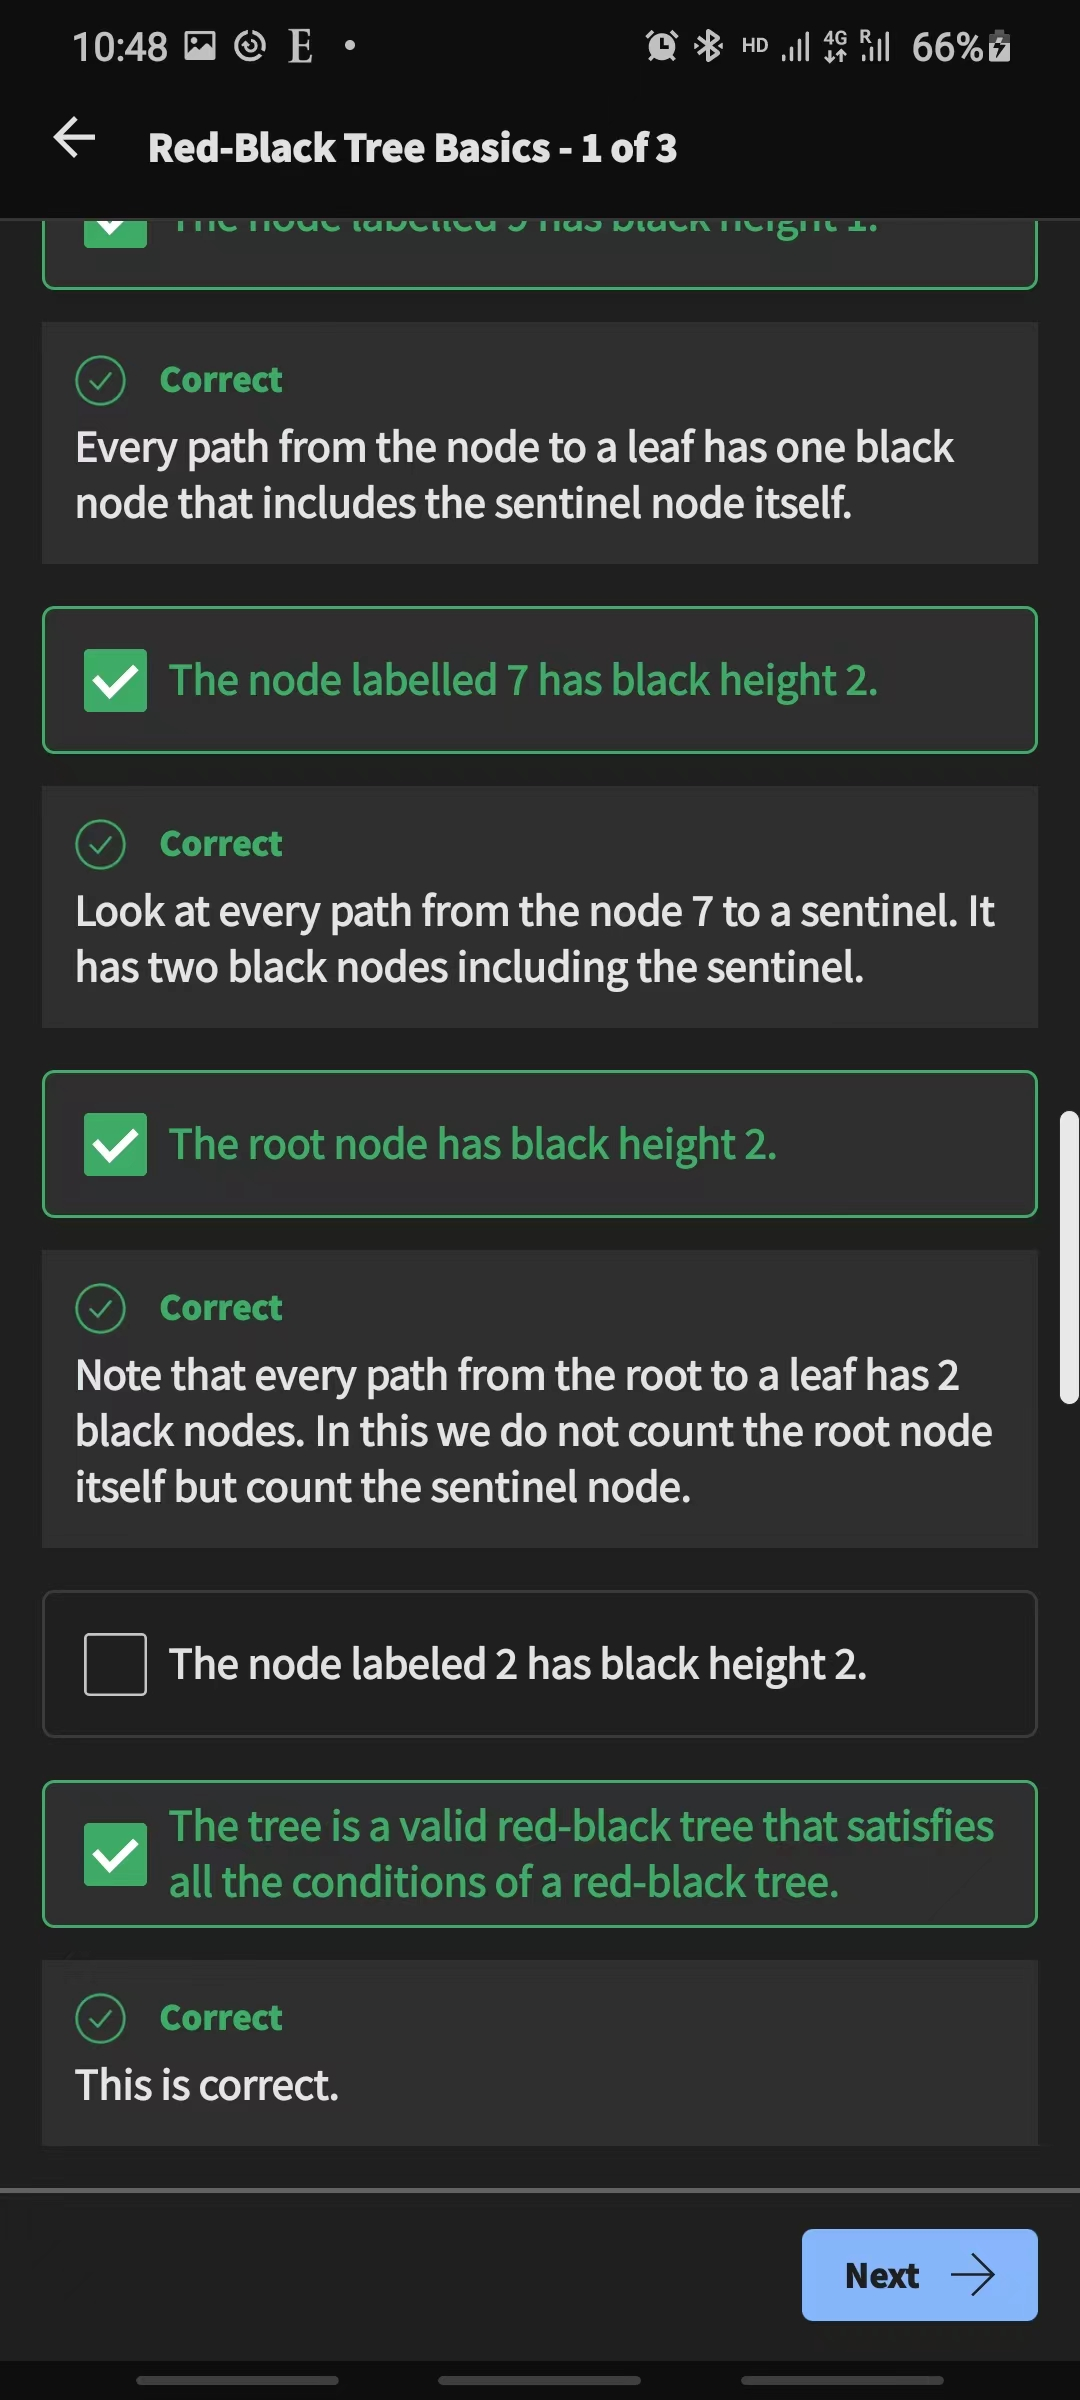
\includegraphics[width=0.45\textwidth]{rbtquiz01-2.jpg}
    }
    \caption{RBT Question 1}
\end{figure}


\begin{figure}[H]
    \centering
    \subfigure{
        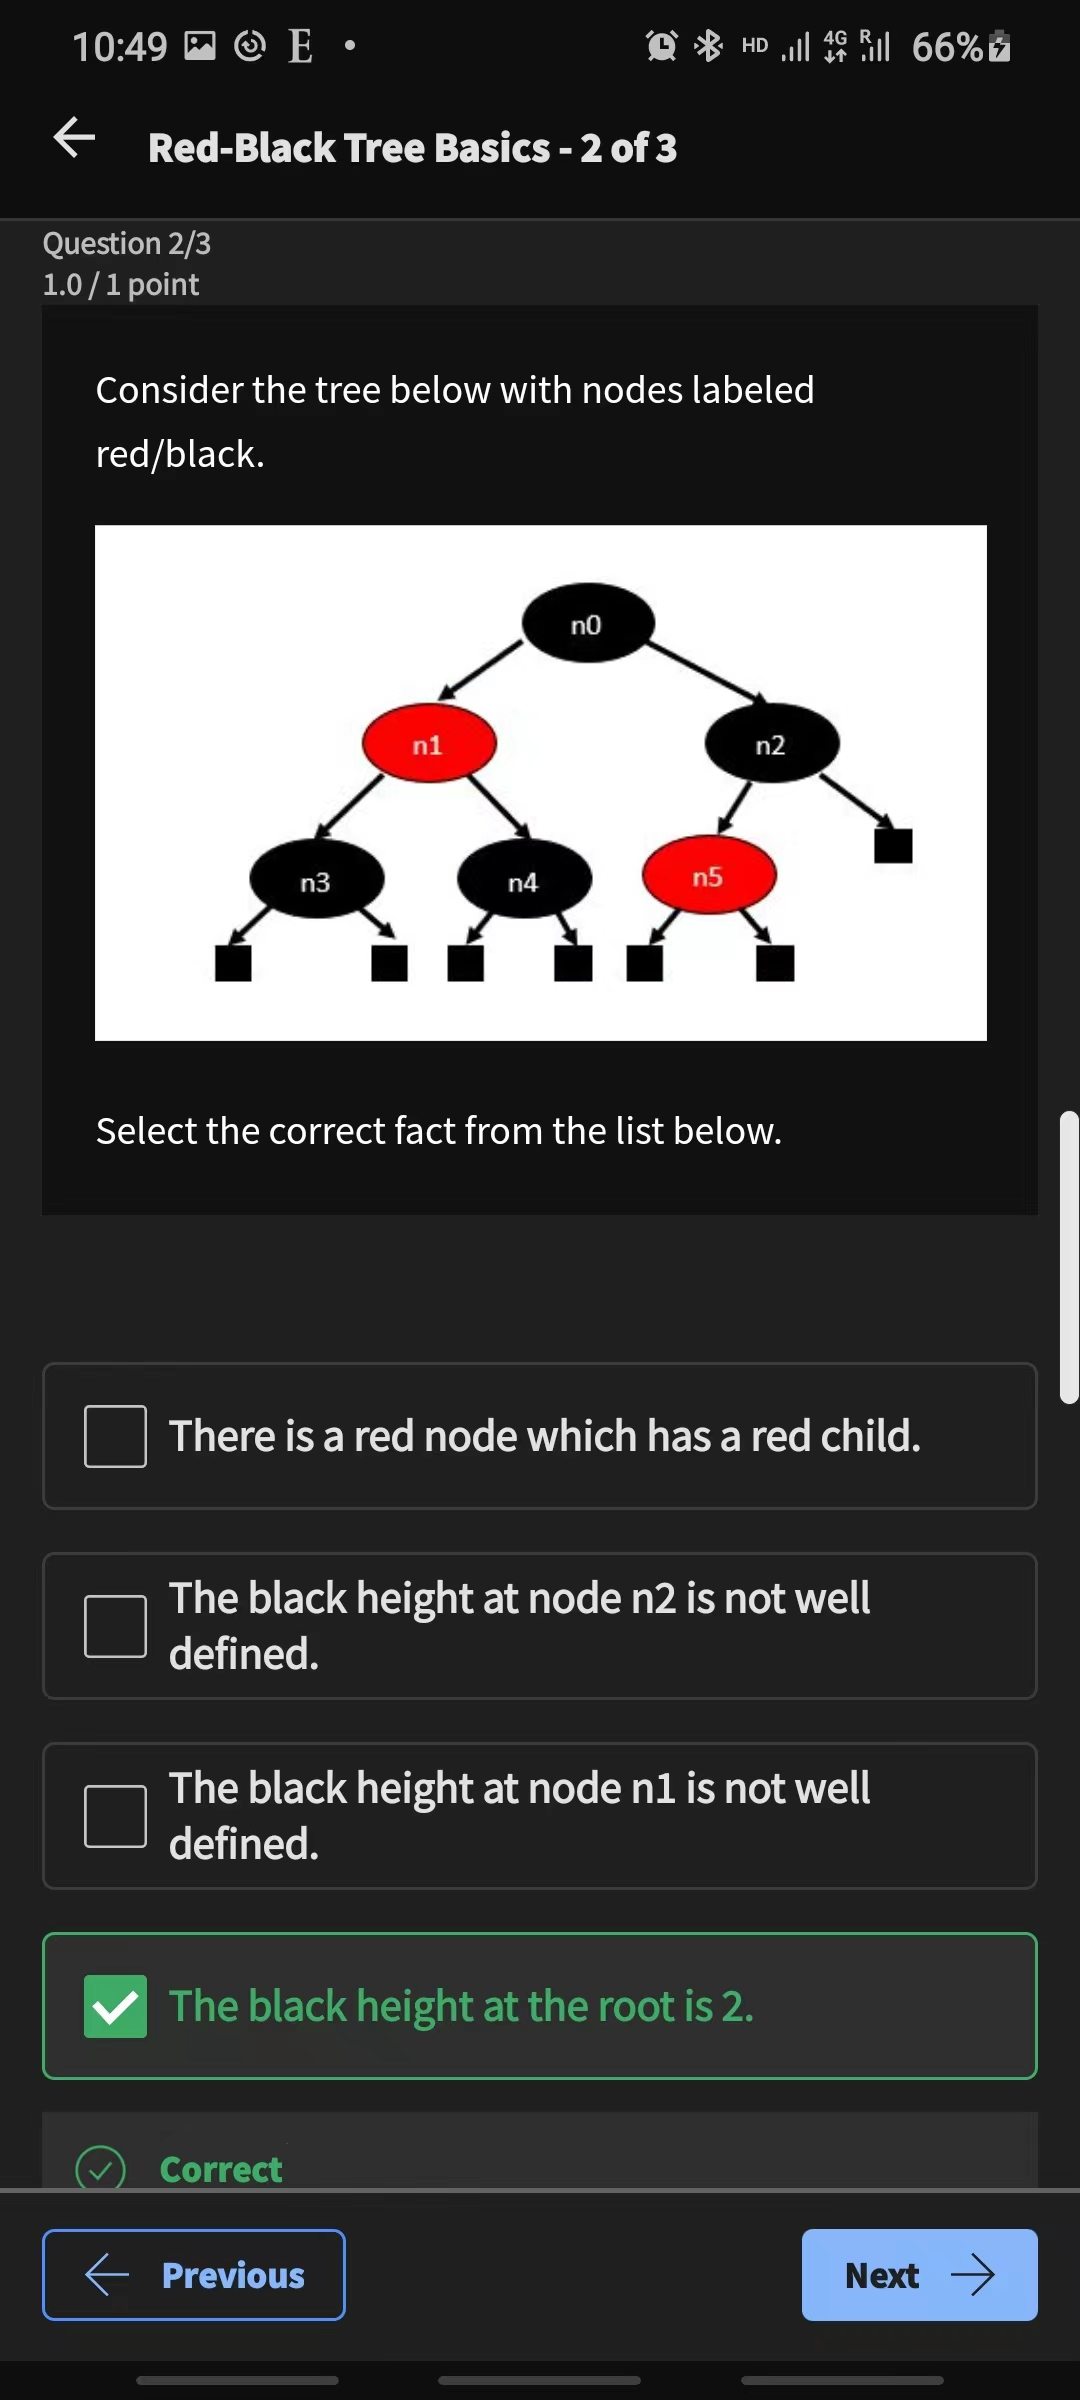
\includegraphics[width=0.45\textwidth]{rbtquiz02.jpg}
    }
    \subfigure{
        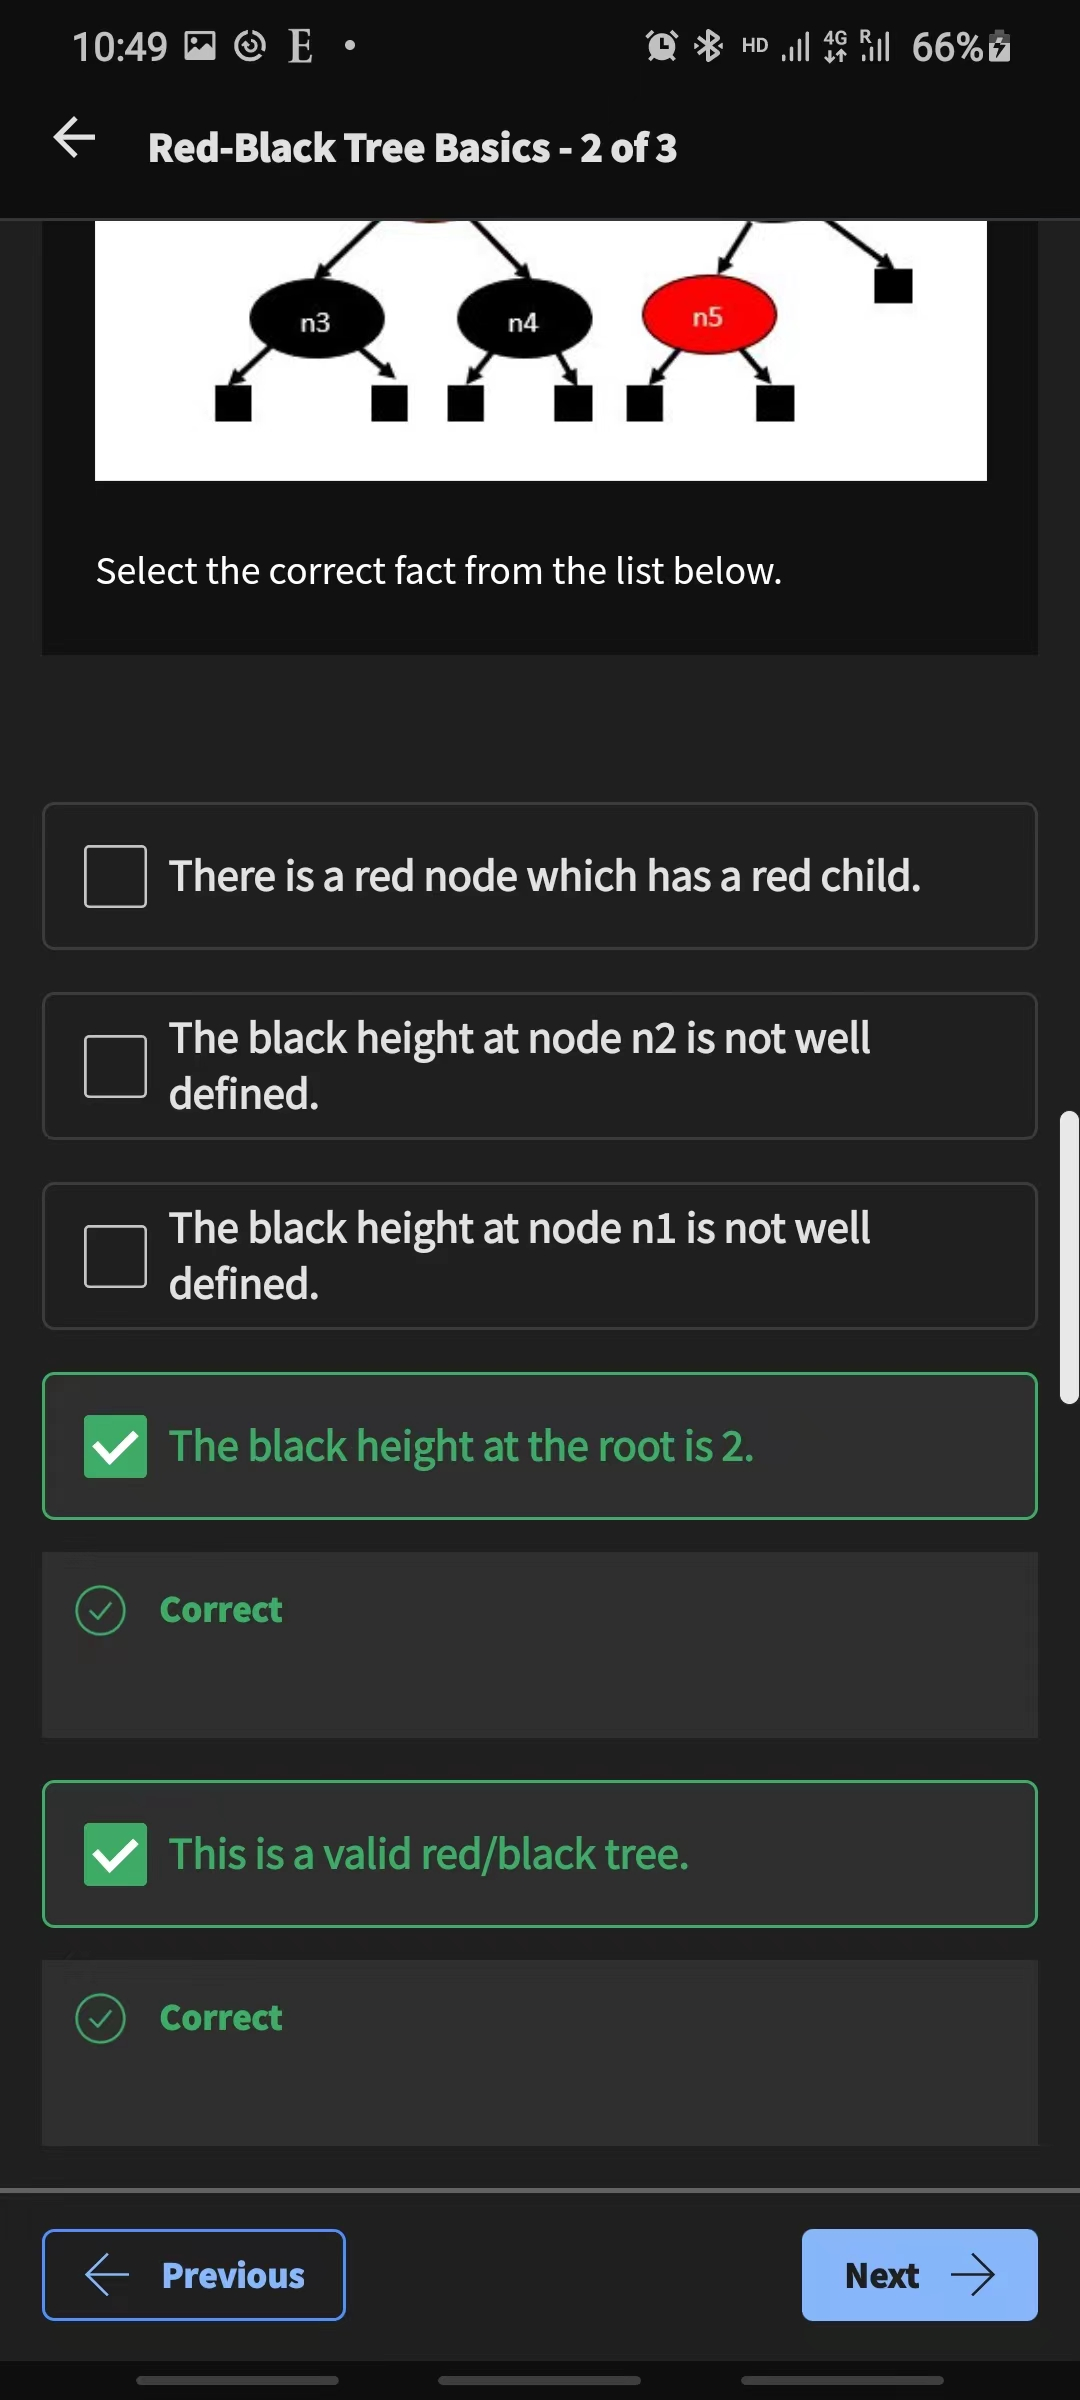
\includegraphics[width=0.45\textwidth]{rbtquiz02-2.jpg}
    }
    \caption{RBT Question 2}
\end{figure}


\begin{figure}[H]
    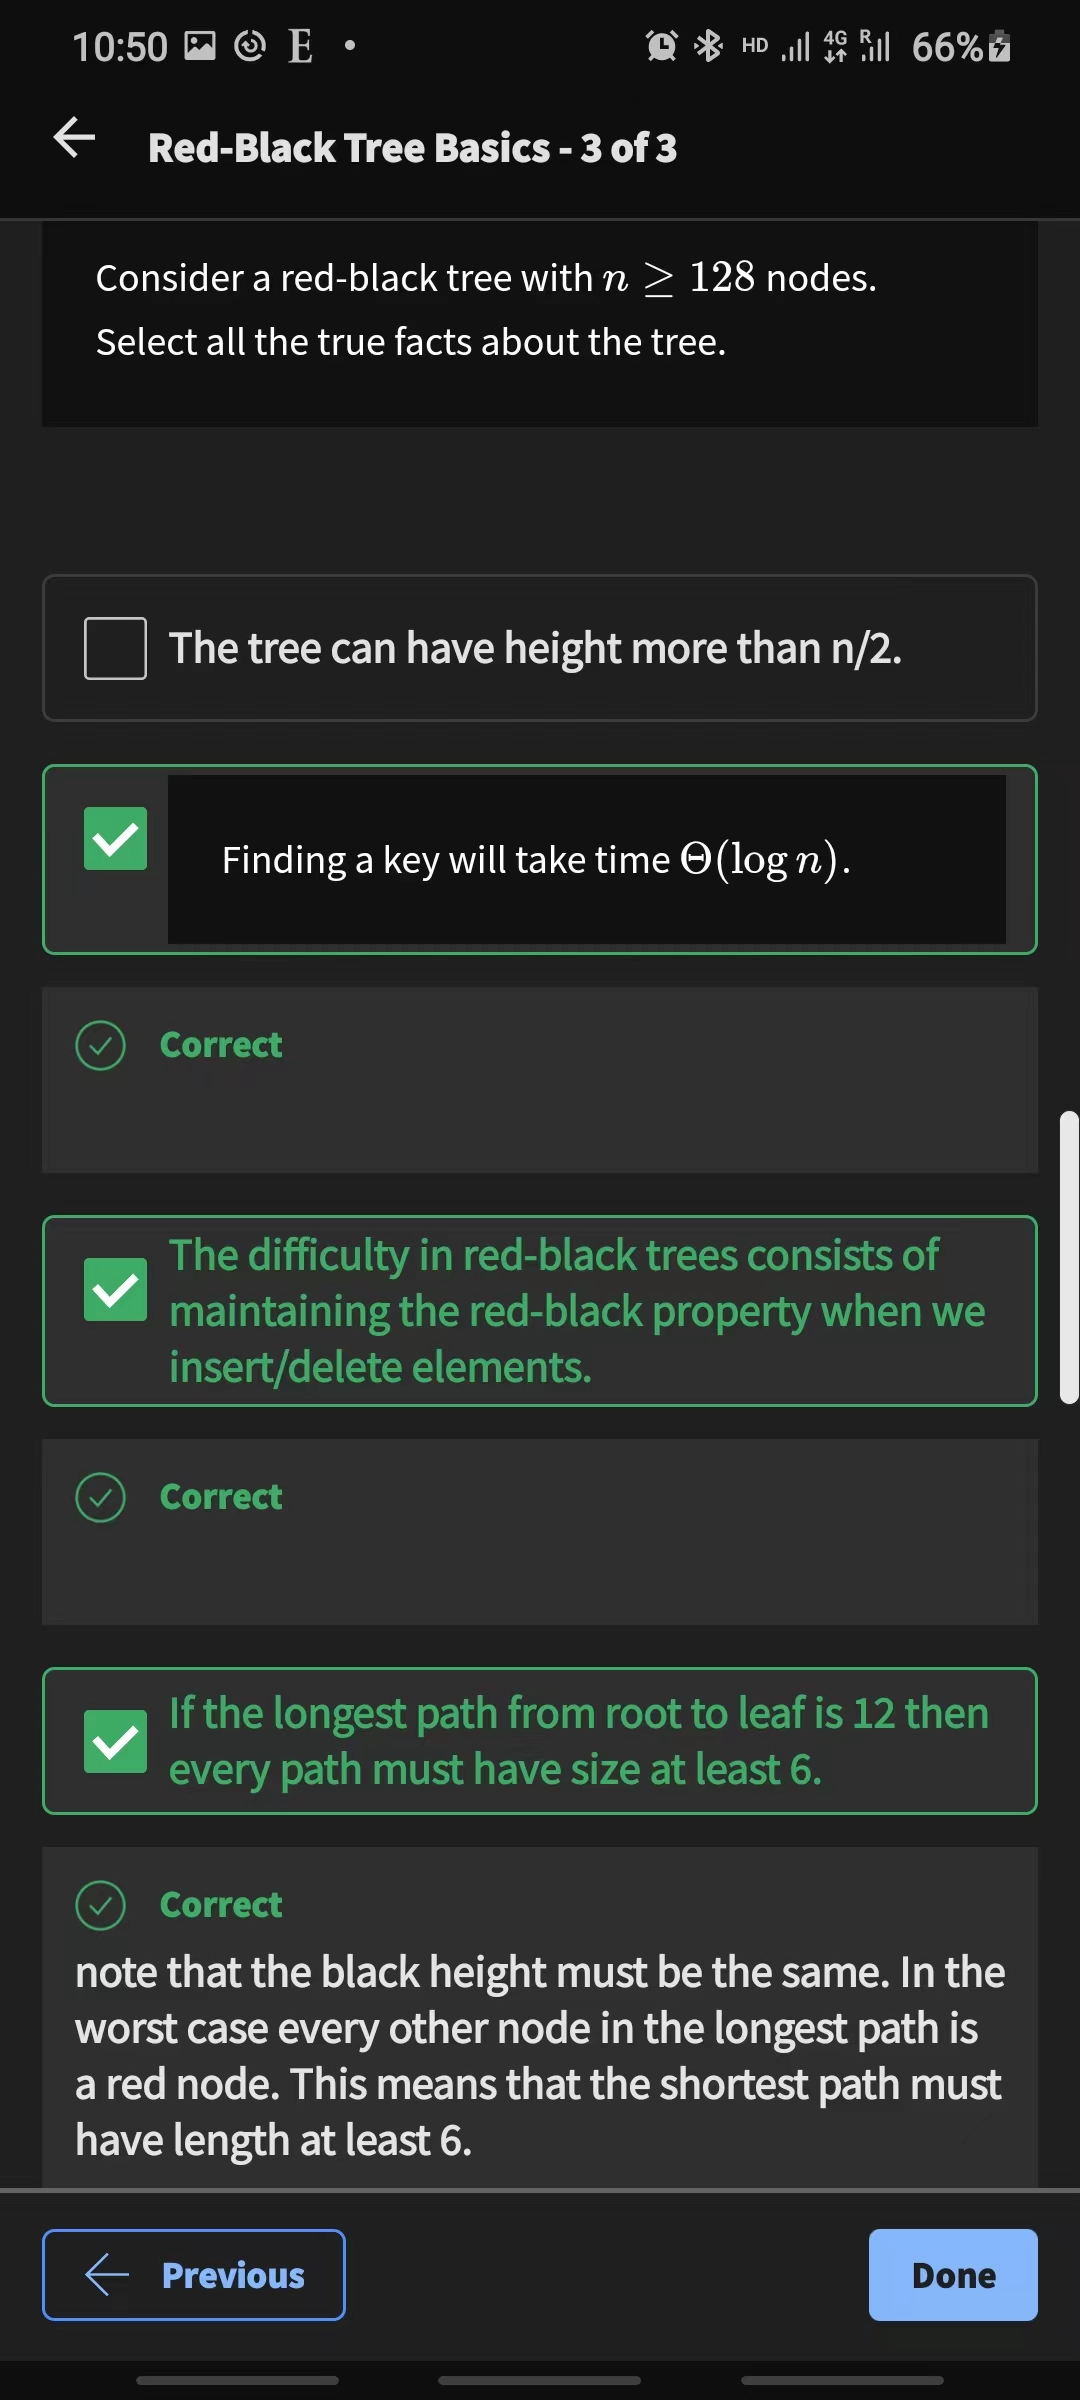
\includegraphics[width=\textwidth]{rbtquiz03.jpg}
    \caption{RBT Question 3}
\end{figure}


\subsection{Red-Black Tree Rotation, Algorithms for Insertion/Deletion}

\paragraph{
    As we know, red-black trees are a type of self-balancing binary search tree.\\
    In order to perform a $find()$ operation, what we do is exactly the same as those of general BSTs.\\
    However, when we insert or delete a node, we need to maintain the red-black tree properties.\\
    To find a particular key in RBT, we will find its height $h$ first.\\
    Then we will find the black height $bh$ of the node.\\
    Since $\theta(h) = \theta(\log_2^n)$, therefore the worst case of running there is $\theta(\log_2^n)$.\\
}

\begin{figure}[H]
    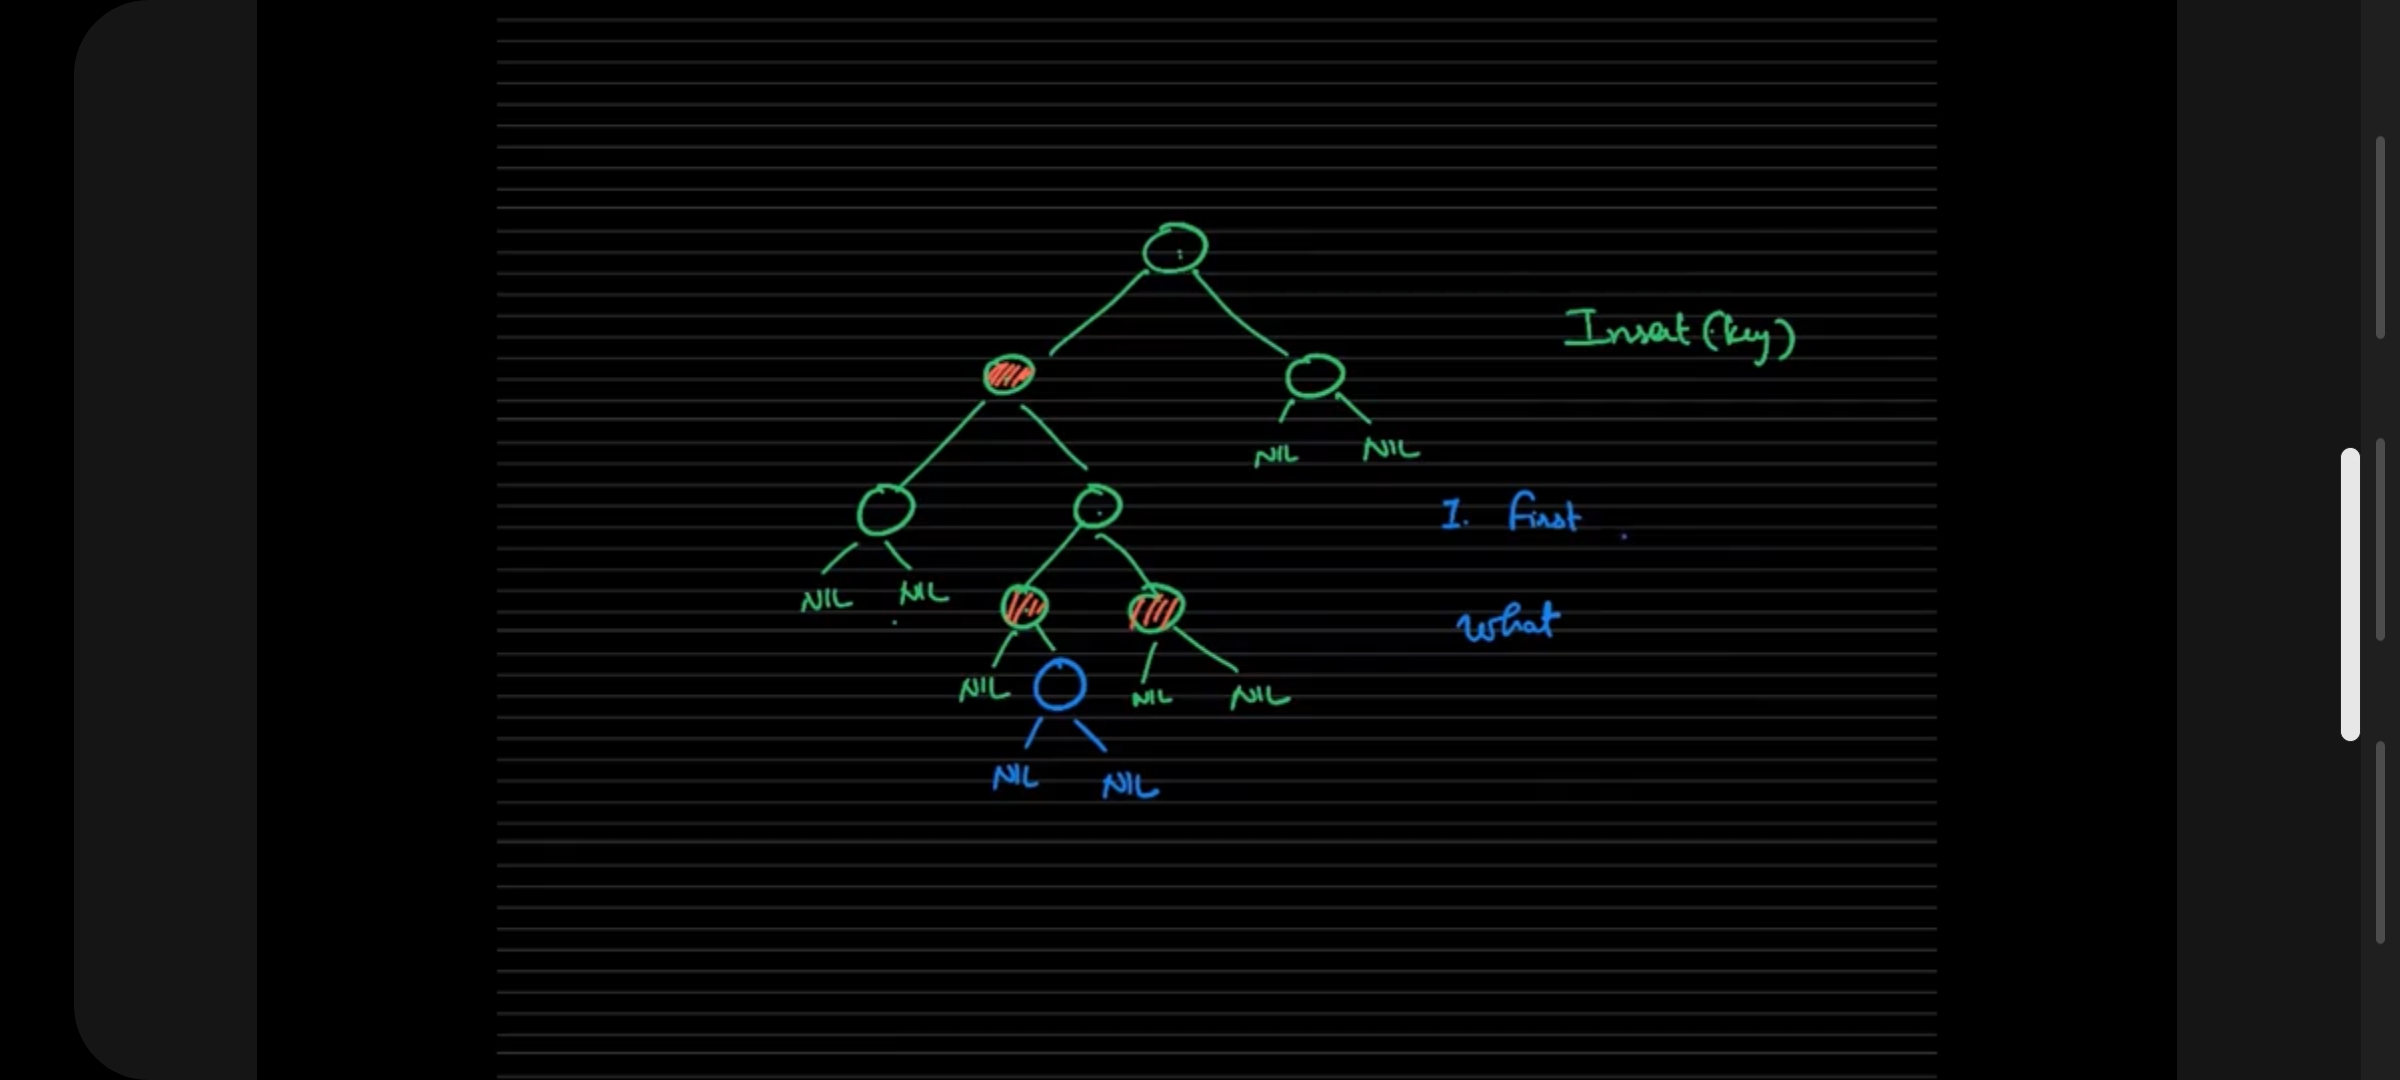
\includegraphics[width=\textwidth]{rbtinsertingakey.jpg}
\end{figure}


\paragraph{
    When performing insert function on RBT, sometimes we encounter a situation where the parent node is red,
    which is called a red-red violation, due to the rule that any inserted nodes will be marked red.\\
    In this case, we need to perform a rotation operation.\\
}

\begin{figure}[H]
    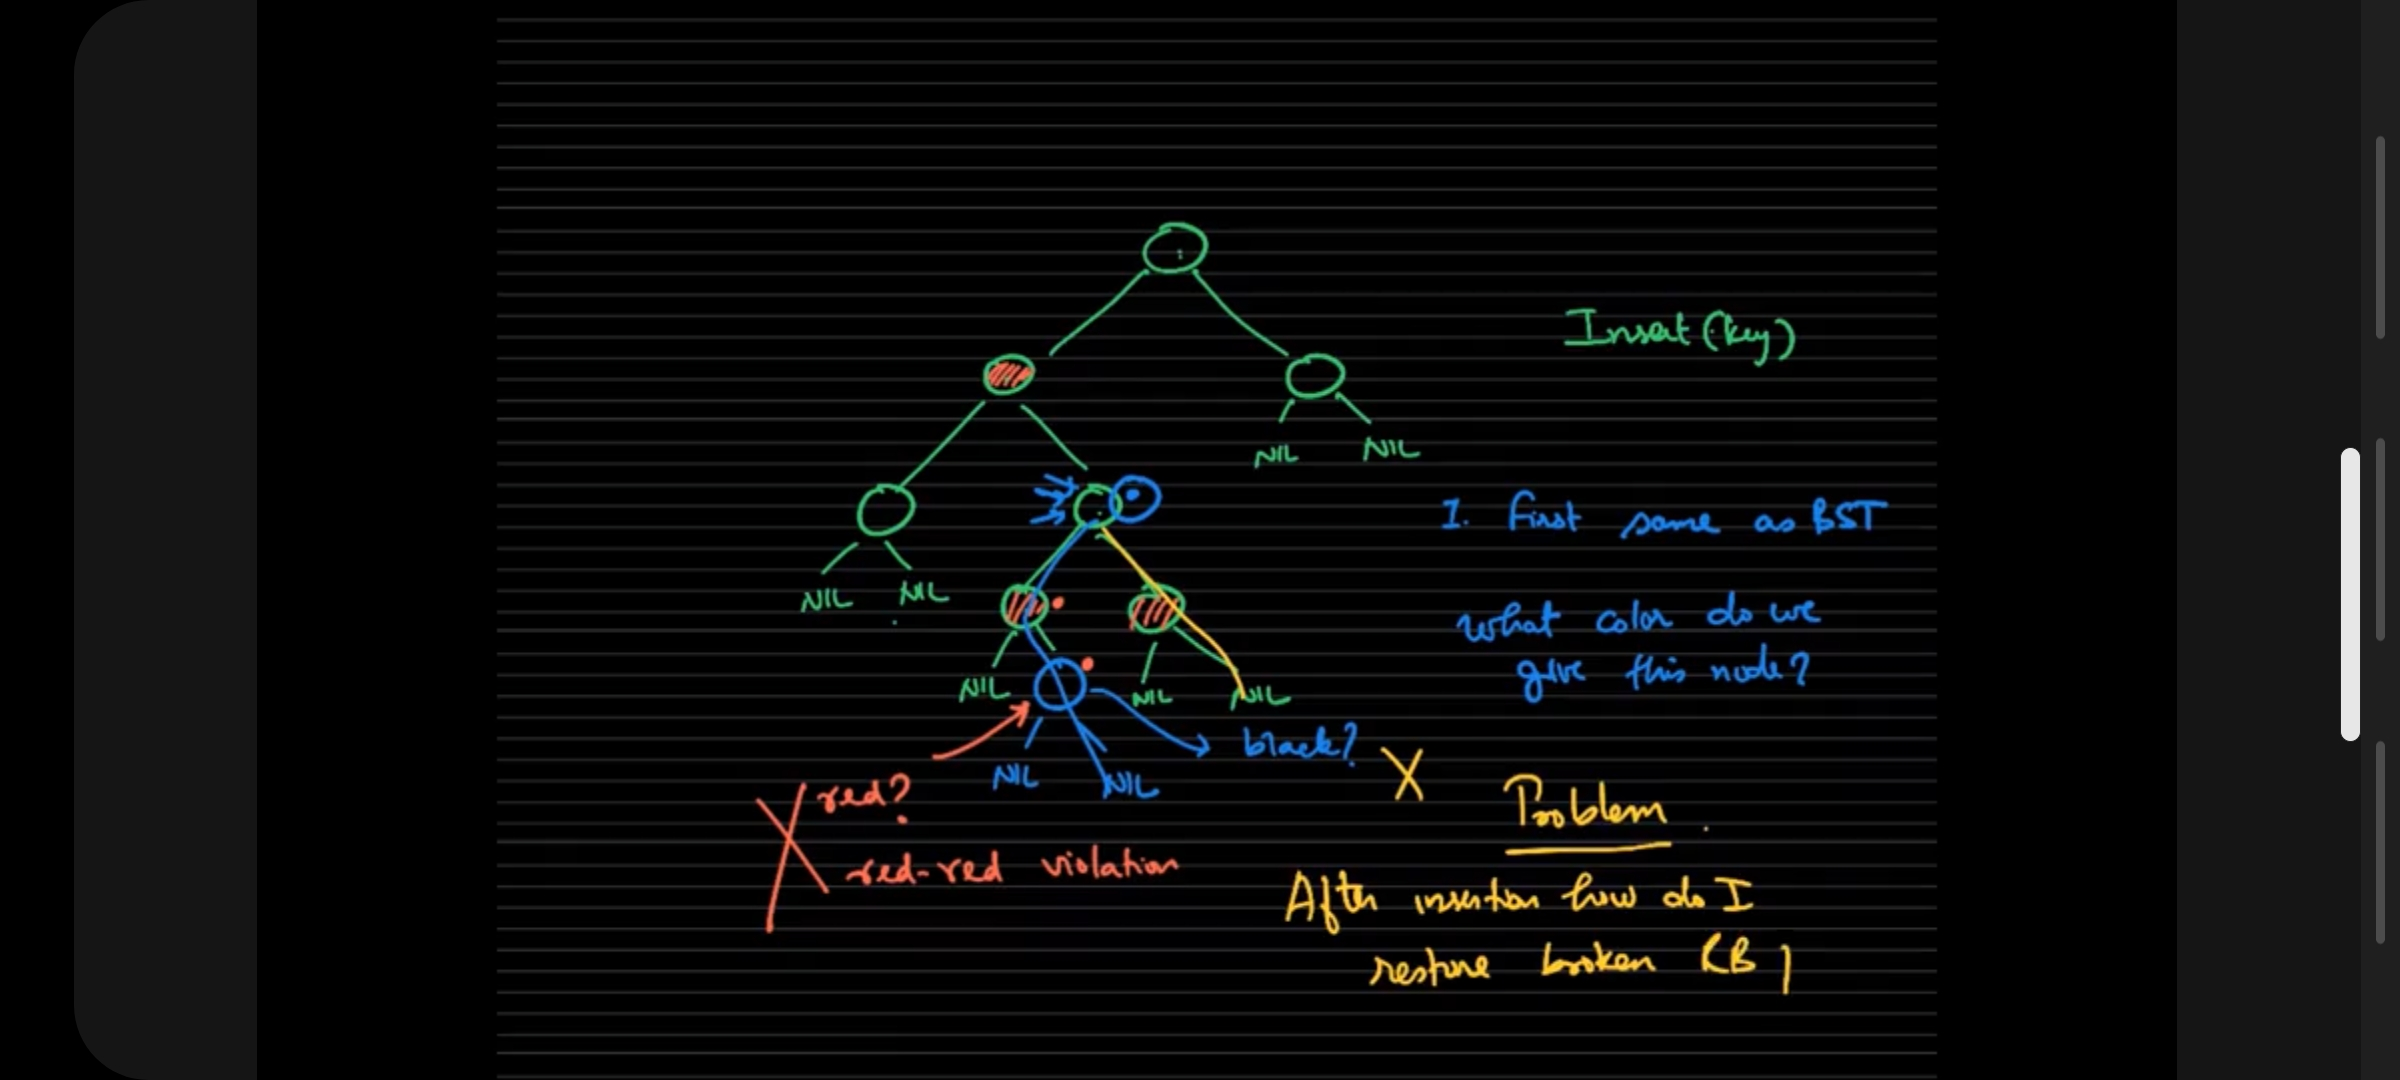
\includegraphics[width=\textwidth]{rbtredredviolation.jpg}
\end{figure}


\paragraph{
    Suppose we have a red-red violation as below.\\
    x is the newly inserted node, y is the parent node of x, and z is the parent node of y.\\
    What we can do is that we  cange the color of y and w to black, and the color of z to red.\\
    Since root node cannot be red, then we need to add a new root node for the tree in order to make it valid.\\
}

\begin{verbatim}
    CASE 1:
    Red-Red Violation Example:
       Root=z
      /   \
    Red=y  Red=w (Uncle of x)
    /       \
  Red=x      Subtree
   / \
 NIL NIL
\end{verbatim}

\begin{verbatim}
    After Color Switch:
       Root=z
      /   \
    Red Root=z
      /   \
 Black=y  Black=w (Uncle of x)
    /       \
  Red=x      Subtree
   / \
 NIL NIL
\end{verbatim}


\paragraph{
    In another case, if node w is black, we need to perform a rotation operation.\\
    There are two types of rotation operations, left rotation and right rotation.\\
    The left rotation operation is as follows.\\
}

\begin{verbatim}
    Left Rotation Example:
       Root=z
      /   \
    Red=y  Black=w
    /       \
  Red=x      Subtree
   / \
 NIL NIL---> This subtree is under x.
\end{verbatim}

\begin{verbatim}
    After Left Rotation:
       Root=y
      /   \
    Red=x  Root=z
    /       /   \
  NIL     Red=w  Subtree
         /   \
       NIL  NIL---> This subtree is now under w, instead of x.
\end{verbatim}


/paragraph{
    If we encounter some unique cases, we need to perform a double rotation as follows.\\
}

\begin{verbatim}
    Double Rotation Example:
       Root=z
      /   \
    Red=y  Black=w
    /       \
  Red=x      Subtree
   / \
 NIL NIL---> This subtree is under x.
\end{verbatim}

\begin{verbatim}
    After Double Rotation:
       Root=x
      /   \
    NIL  Root=z
         /   \
       Red=y  Subtree
       /   \
     NIL  Red=w
         /   \
       NIL  NIL---> This subtree is now under w, instead of x.
\end{verbatim}

\begin{figure}[H]
    \centering
    \subfigure{
        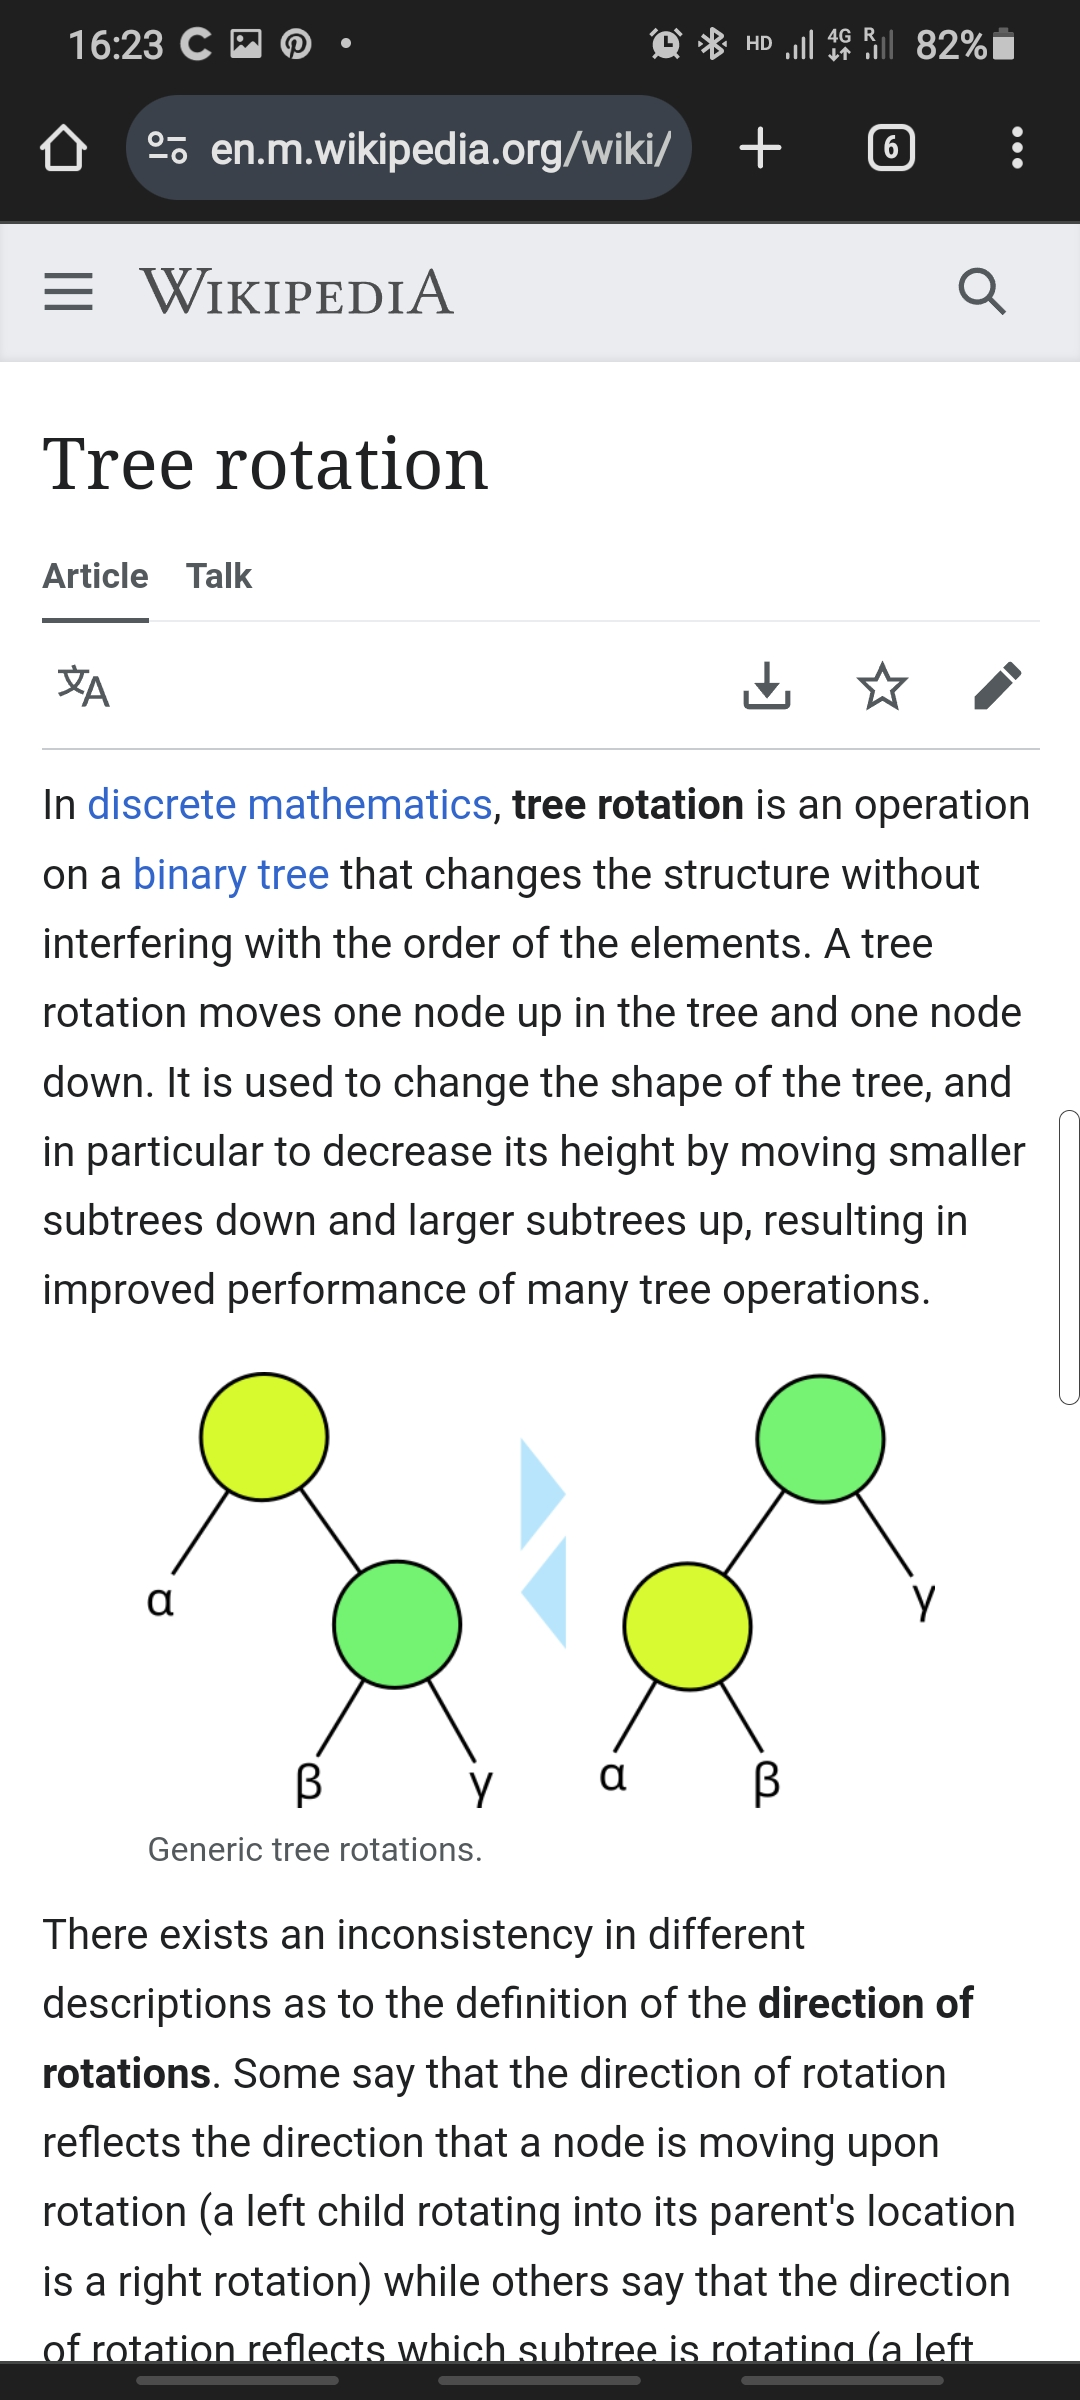
\includegraphics[width=0.45\textwidth]{wikipediatreerotation.jpg}
    }
    \subfigure{
        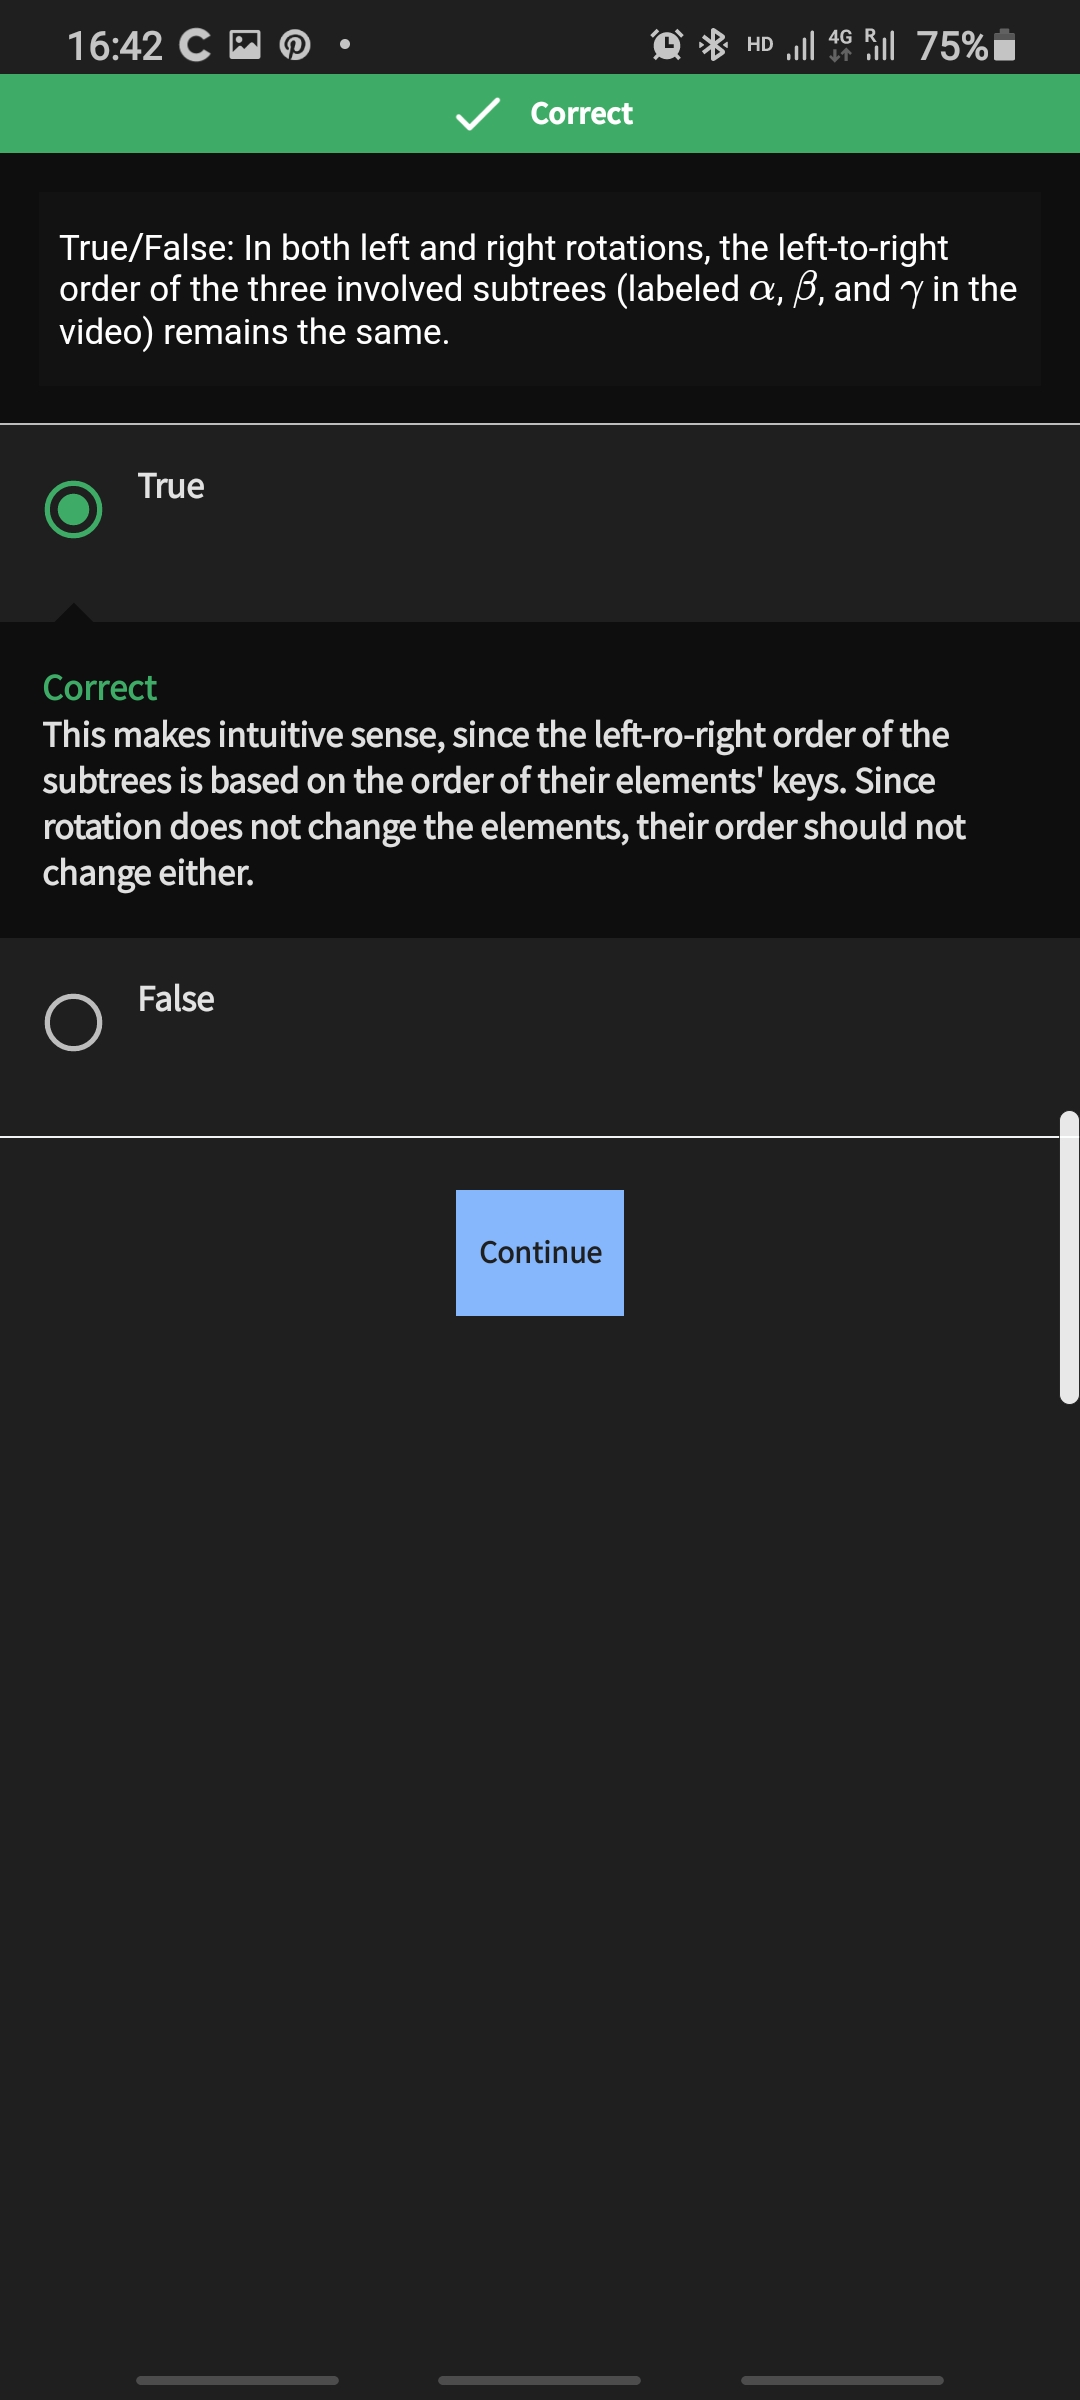
\includegraphics[width=0.45\textwidth]{treerotationquestion.jpg}
    }
    \caption{Wikipedia Tree Rotation Explanation}
\end{figure}


\begin{figure}[H]
    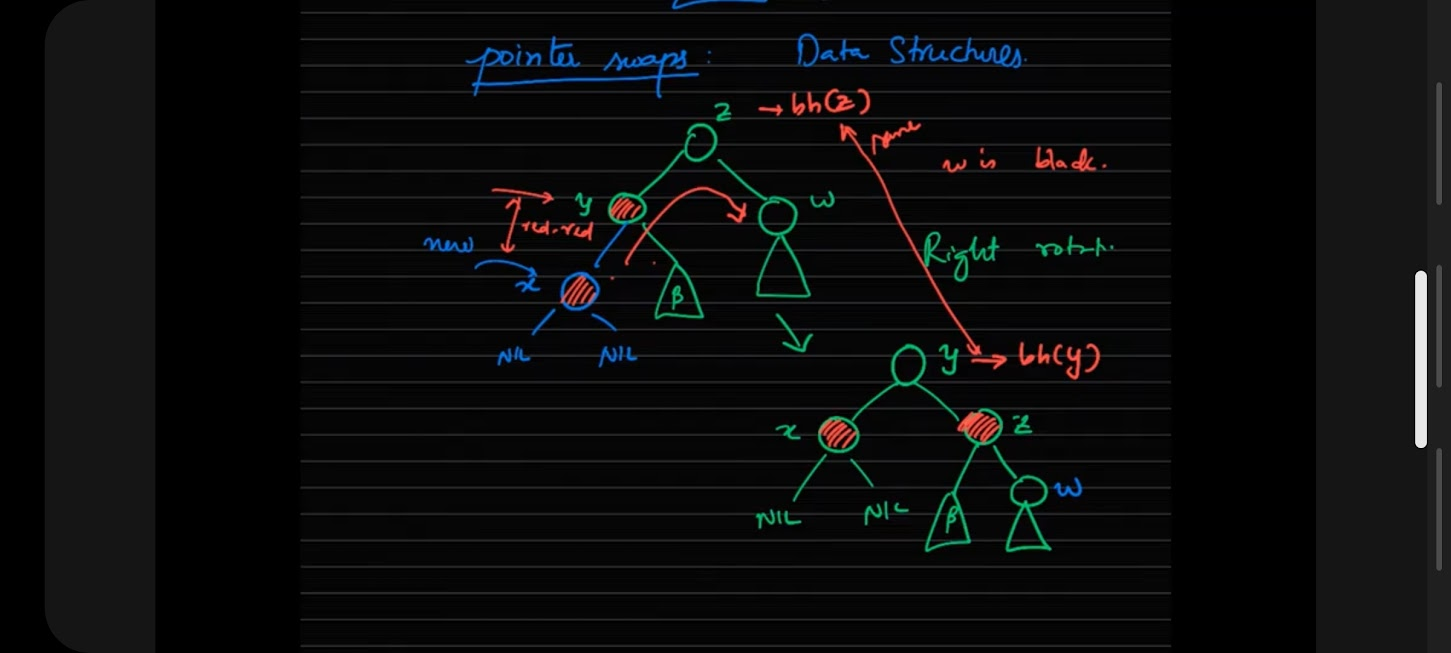
\includegraphics[width=\textwidth]{afterrightrotation.jpg}
\end{figure}

\paragraph{
    If we encounter some unique cases, we need to perform a double rotation as follows.\\
}

\begin{verbatim}
        Double Rotation Example:
        Root=z
        /   \
     Red=y  Black=w
       /\
Subtree Red=x   
\end{verbatim}

\paragraph{
    Firstly, we will do a left rotation on the x and y subtree section.\\
}

\begin{verbatim}
    After first rotation:
        Root=z
        /   \
     Red=x  Black=w
       /\
 Red=y   Subtree
\end{verbatim}

\paragraph{
    Then we will do a right rotation on the z and x subtree section.\\
}

\begin{verbatim}
    After second rotation:
        Root=x
        /   \
     Red=y  Red=z
             /  \ 
         Subtree  w
\end{verbatim}

\paragraph{
    Now we can see that the tree is a valid red-black tree.\\
}

\paragraph{
    Insertion and deletion both has the complexity of $O(\log_2^n)$.\\
    This is not too much of the problem, the problem is that we need to maintain the red-black tree properties after each insertion and deletion.\\
    This is not easy to do, and we need to be careful to ensure that the tree remains balanced and valid after each operation.\\
}


\begin{figure}[H]
    \centering
    \subfigure{
        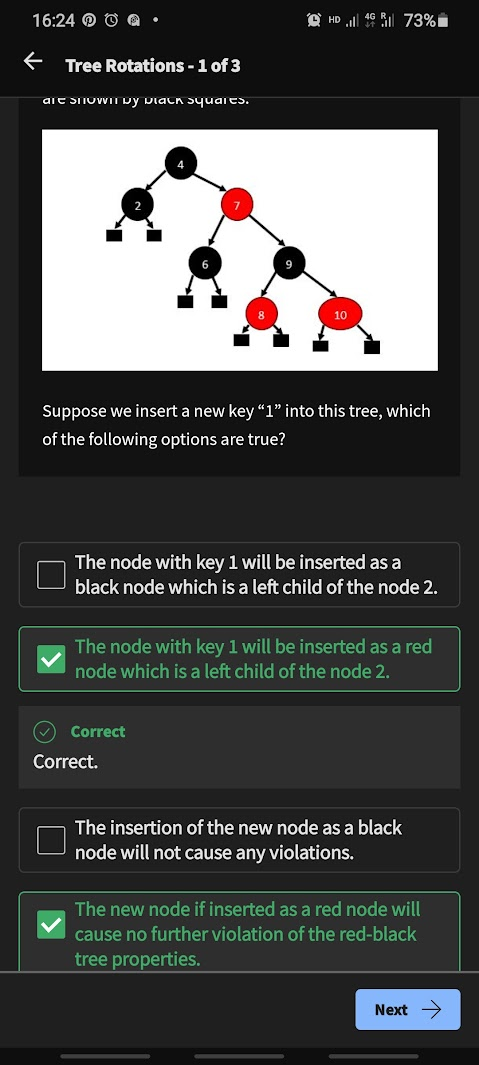
\includegraphics[width=0.3\textwidth]{rotationquiz1.jpg}
    }
    \subfigure{
        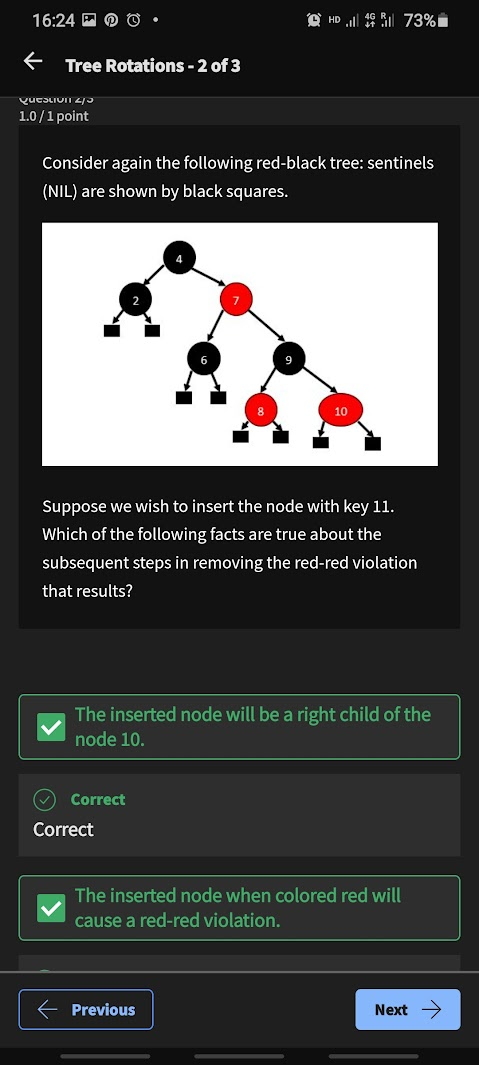
\includegraphics[width=0.3\textwidth]{rotationquiz2-1.jpg}
    }
    \subfigure{
        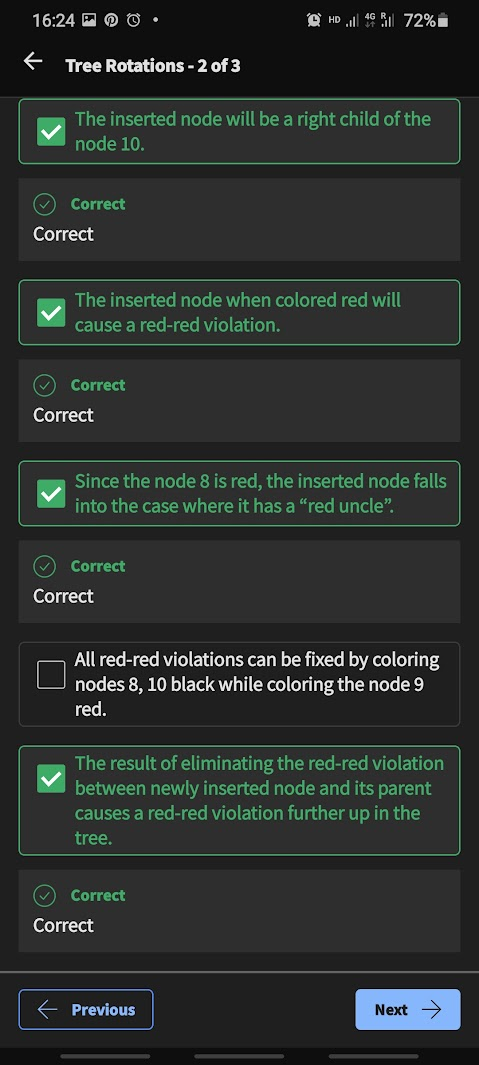
\includegraphics[width=0.3\textwidth]{rotationquiz2-2.jpg}
    }
    \caption{Tree Rotation Quiz}
\end{figure}


\subsection{Skip Lists}

\paragraph{
    Skip lists are a data structure that provides an alternative to balanced trees for implementing dictionaries.\\
    They are similar to balanced trees in that they maintain a sorted list of keys, but they use a different approach to achieve balance.\\
    In a skip list, each node has a level, and the level of a node is determined by the number of nodes in the list that are above it.\\
    The higher the level of a node, the more nodes it has above it.\\
    The levels of the nodes form a staircase pattern, with each level being a power of 2.\\
    The height of the skip list is the number of levels in the highest node.\\
}


\begin{figure}[H]
    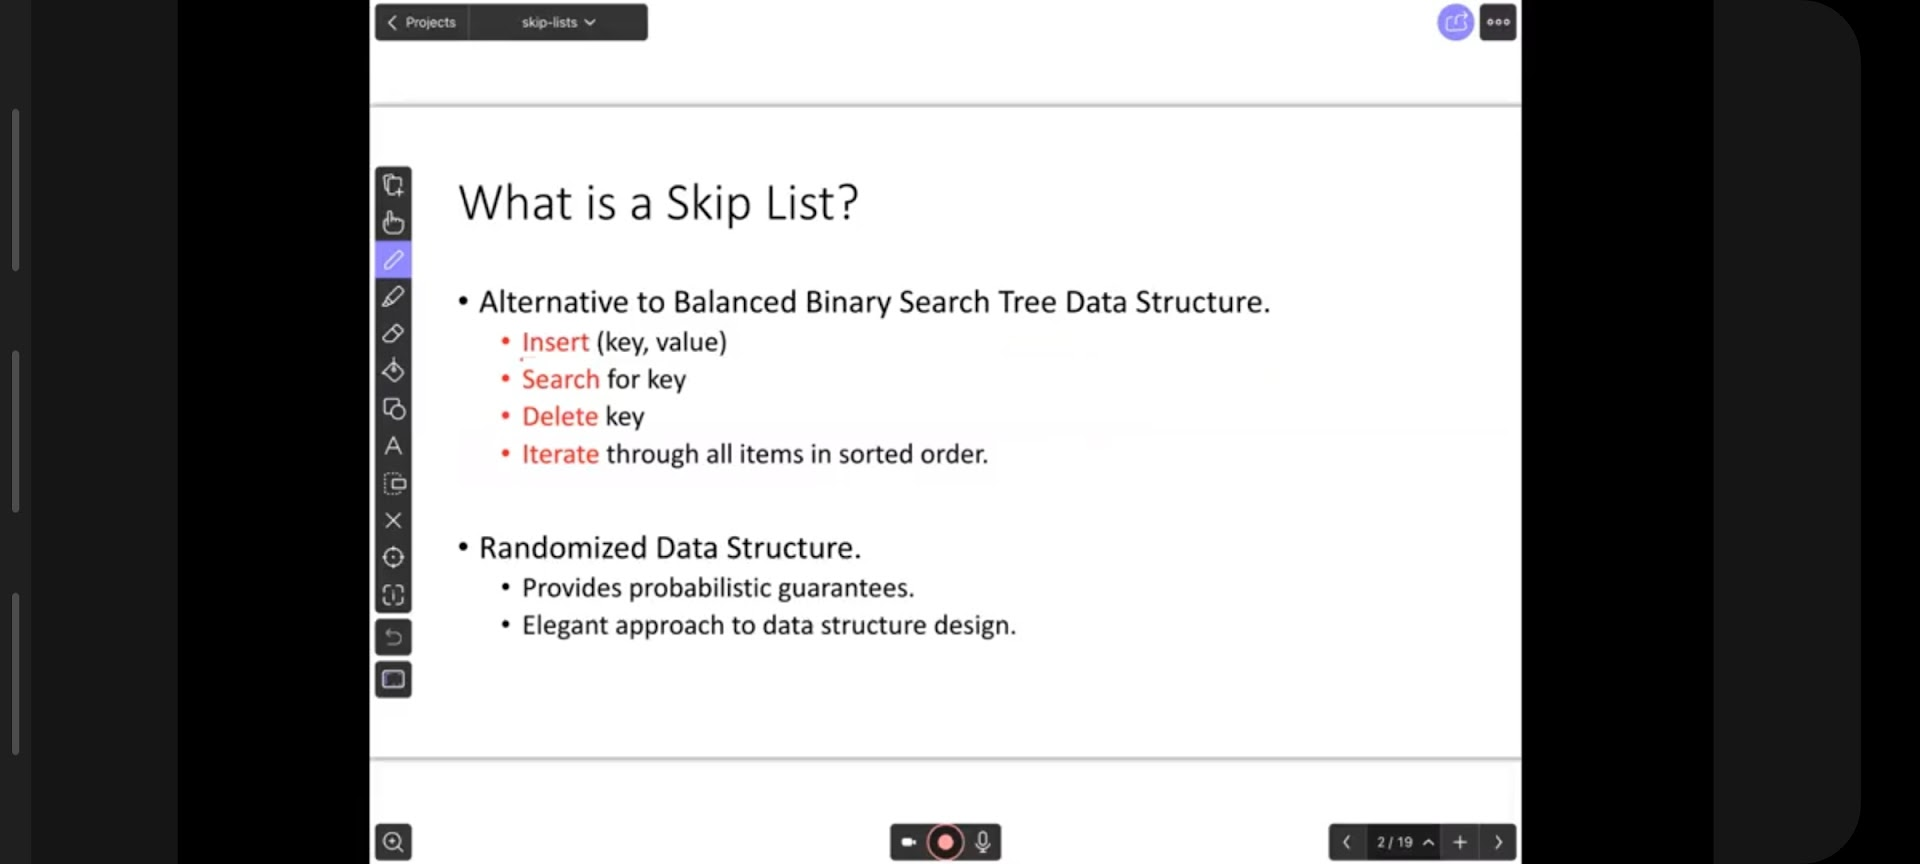
\includegraphics[width=\textwidth]{whatisaskiplist.jpg}
\end{figure}

\begin{figure}[H]
    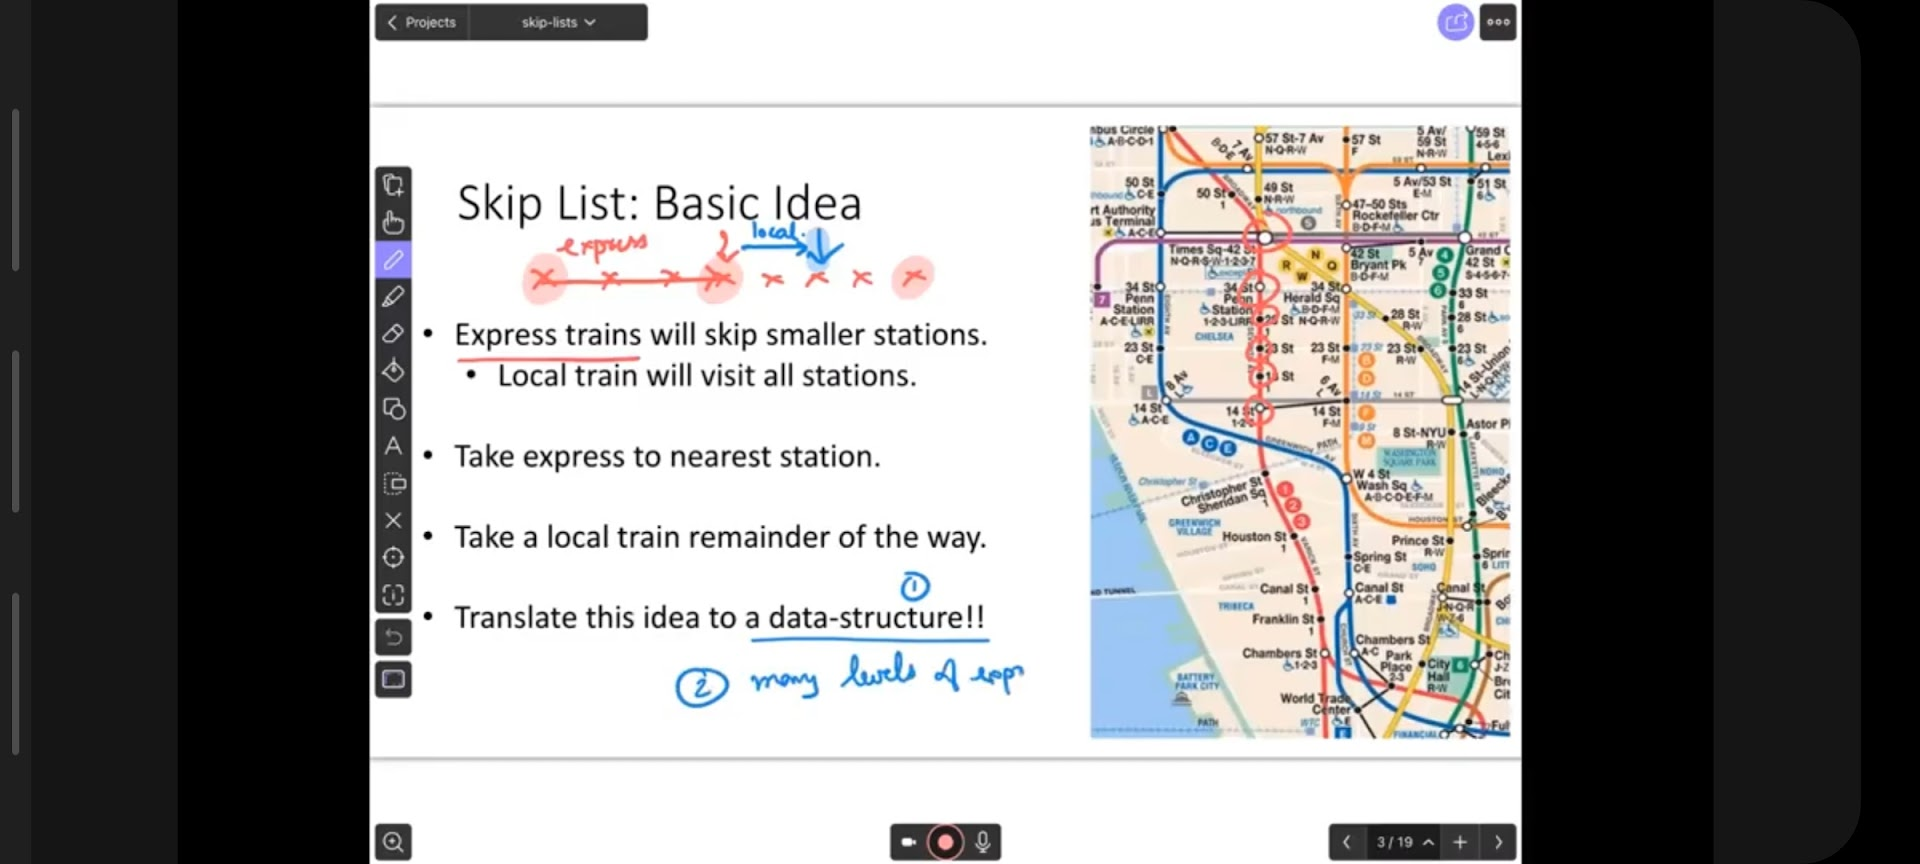
\includegraphics[width=\textwidth]{skiplistmapexample.jpg}
\end{figure}


\paragraph{
    For any layer in the skip list, the elements are sorted in ascending order from left to right.\\
    The elements in the lower layer are the elements in the higher layer, plus some extra elements in between.\\
    The extra elements are the ones that are not in the lower layer. Therefore, all the top layers are just subsets of the bottom layer.\\
}

\begin{figure}[H]
    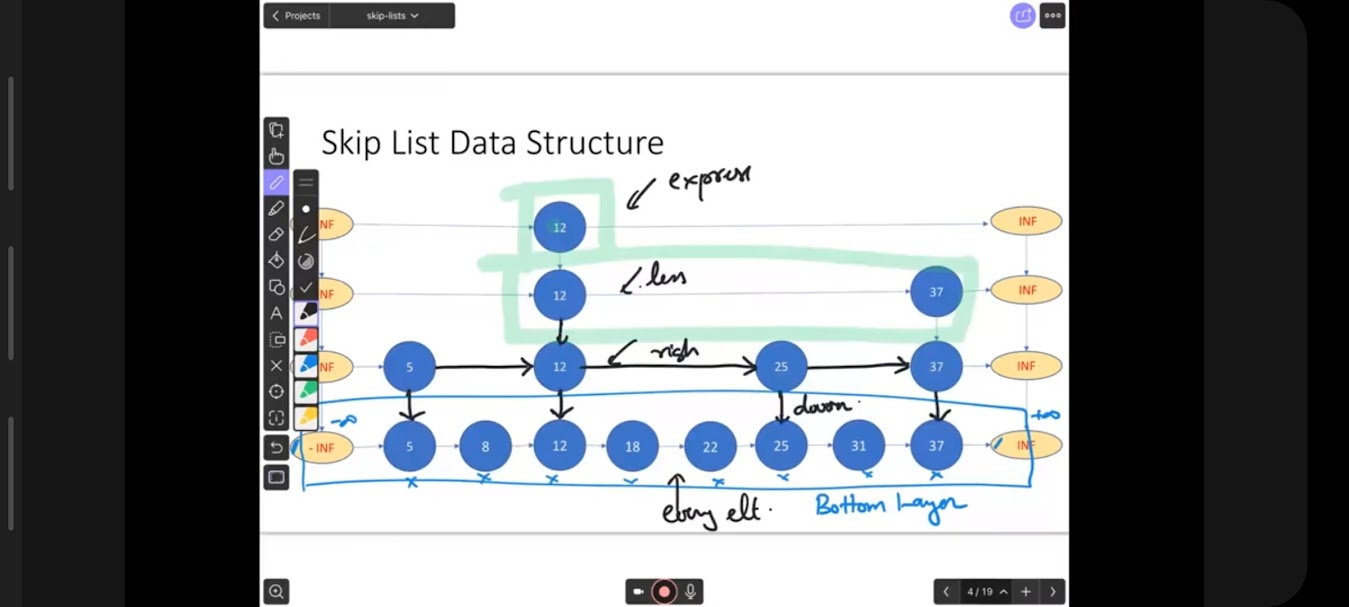
\includegraphics[width=\textwidth]{skiplistdatastructure.jpg}
\end{figure}


\paragraph{
    How do we use skip lists to implement dictionaries?
    We can use the following operations:\\
    1. $find()$: Find the node with the given key in the skip list.\\
    2. $insert()$: Insert a new node with the given key into the skip list.\\
    3. $delete()$: Delete the node with the given key from the skip list.\\
    How does the $find()$ operation work?
    We start from the topmost layer of the skip list, and we will compare the key with the current node.\\
    If the key is greater than the current node, we will move to the right to the next node in the same layer.\\
    If the key is less than the current node, we will go back to the previous node in the same layer, and move down to the next node in the lower layer.\\
    We will continue this process until we reach the bottommost layer.\\
    If we reach the bottommost layer and still cannot find the key, we will return NIL.\\
}

\begin{figure}[H]
    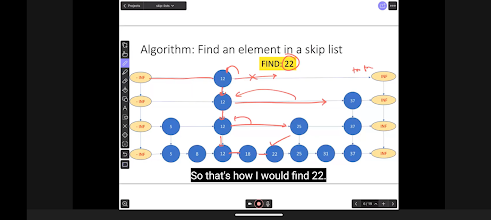
\includegraphics[width=\textwidth]{skiplistfind22.png}
\end{figure}

\begin{figure}[H]
    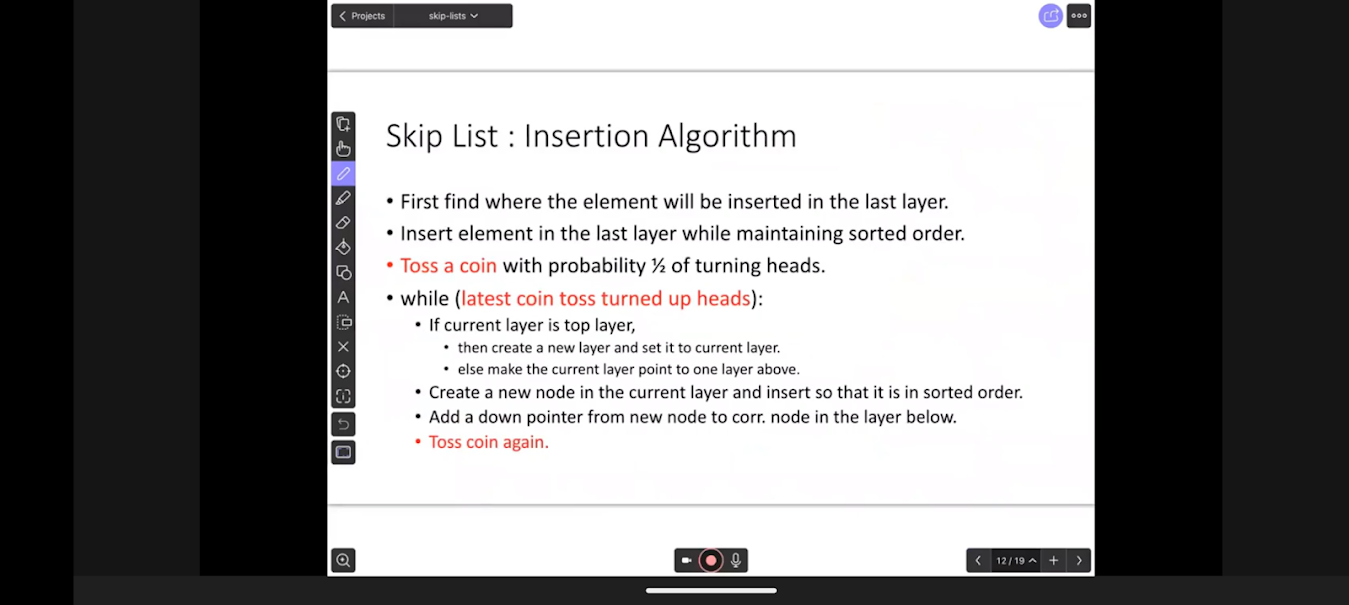
\includegraphics[width=\textwidth]{skiplistinsertion.png}
\end{figure}

\paragraph{
    What is the average height of a skip list?\\
    The average height of a skip list is $O(\log_2^n)$.\\
    This is because the height of a skip list is determined by the number of levels in the highest node, and the number of levels in the highest node is $O(\log_2^n)$.\\
}

\paragraph{
    The probability of a node exceeding height $h$ is $(1/2)^h$.\\
    This is because the probability of a node exceeding height $h$ 
    is the probability of a node exceeding height $h-1$, and the probability 
    of a node exceeding height $h-1$ is $1/2^{h-1}$.\\
    Therefore, the probability of a node exceeding height $h$ is $(1/2)^h$.\\
}

\begin{figure}[H]
    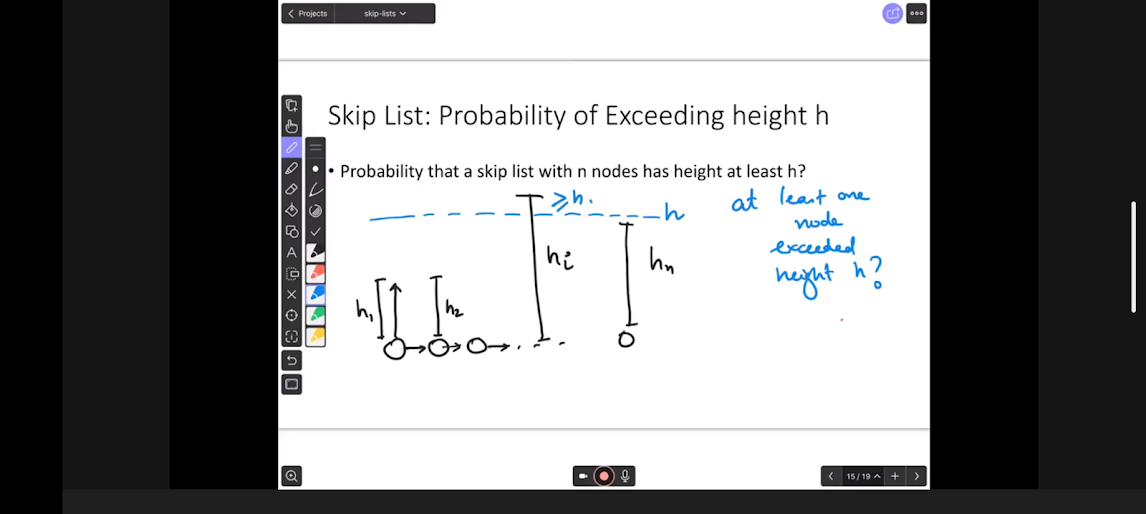
\includegraphics[width=\textwidth]{skiplistheightexceedingh.png}
\end{figure}

\paragraph{
    This is similar to the Boolie's inequality in probability theory.\\
    Boolie's inequality is a probability inequality that bounds the probability 
    of the union of events by the sum of the probabilities of the individual events.\\
    In this case, the events are the nodes exceeding height $h$, and the probability of 
    a node exceeding height $h$ is $(1/2)^h$.\\
    The sum of the probabilities of the events is the expected height of the skip list.\\
    Therefore, the expected height of the skip list is $O(\log_2^n)$.\\
    $P(>h) \leq \sum_{i=h}^{\infty} P(i) = \sum_{i=h}^{\infty} (\frac{1}{2})^i = \frac{1}{2^h}$.\\
}


\begin{figure}[H]
    \centering
    \subfigure{
        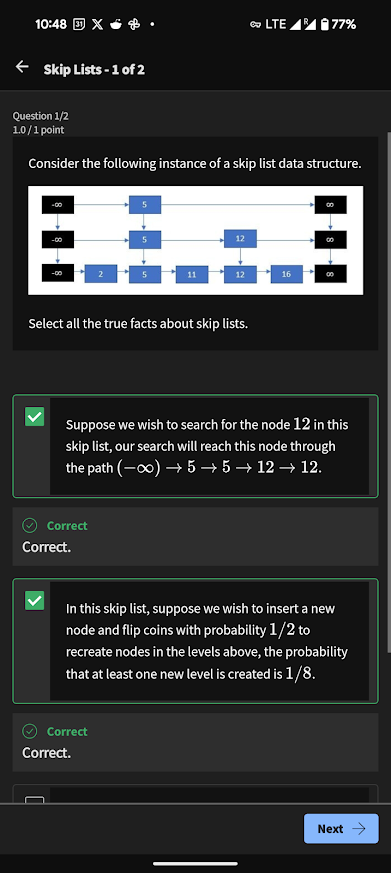
\includegraphics[width=0.3\textwidth]{skiplistquiz1.png}
    }
    \subfigure{
        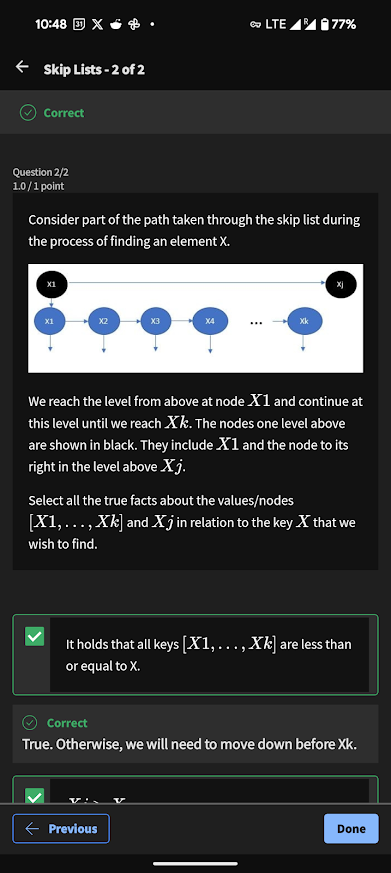
\includegraphics[width=0.3\textwidth]{skiplistquiz2-1.png}
    }
    \subfigure{
        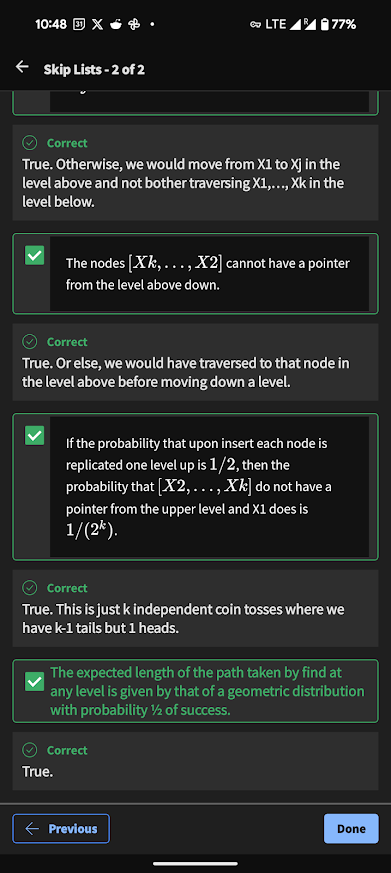
\includegraphics[width=0.3\textwidth]{skiplistquiz2-2.png}
    }
    \caption{Skip List Quiz}
\end{figure}




\section{Graphs}

\subsection{Graphs and Their Representations}

\paragraph{
    A graph is a data structure that consists of a set of vertices and a set of edges.\\
    The vertices are the nodes of the graph, and the edges are the connections between the nodes.\\
    There are two types of graphs: directed graphs and undirected graphs.\\
    In a directed graph, the edges have a direction, and in a undirected graph, the edges do not have a direction.\\
    Normally we don't consider the self-loop in the graph. There should be no multi-edges between vectices.\\
}

\paragraph{
    Where do graph come from?\\
    Graphs are used to model relationships between objects.\\
    For example, a social network can be represented as a graph, where the vertices are the people in the network and the 
    edges are the connections between the people.\\
    Graphs are also used to model networks, such as the internet (computer network), where the vertices are the computers in the network and the
    edges are the connections between the computers.\\
    Other networks such as Ecological networks, electrical circuits, and transportation networks can also be represented as graphs.\\
    How do we represent a graph in a computer?\\
    There are two common ways to represent a graph in a computer: adjacency matrix and adjacency list.\\
    The adjacency matrix is a 2D array that stores the connections between the vertices.\\
    The row and column indices are actually vertices, when there's an edge, the value will be 1, otherwise 0.\\
}

\begin{figure}[H]
    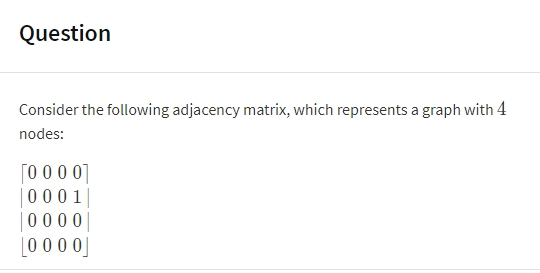
\includegraphics[width=\textwidth]{graphquestion1-1.png}
\end{figure}

\begin{figure}[H]
    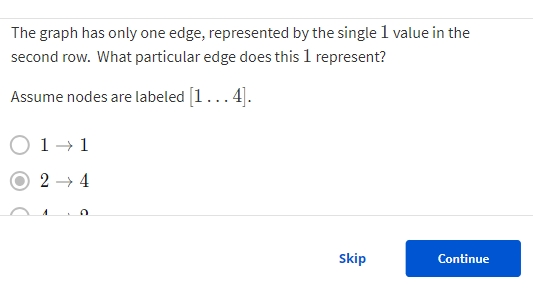
\includegraphics[width=\textwidth]{graphquestion1-2.png}
\end{figure}

\paragraph{
    For a graph with $k$ nodes, the adjacency matrix will be a $k*k$ matrix.\\
    There will be up to $k(k-1)$ edges in the graph.\\
    Then we come to the adjacency list.\\
    The adjacency list is a list of lists that stores the connections between the vertices.\\
    Each vertex has a list of its neighbors.\\
    The adjacency list is more space-efficient than the adjacency matrix, 
    especially for sparse graphs.\\
    The adjacency list is also more time-efficient for some operations, 
    such as finding the neighbors of a vertex.\\
    Here is a example as denoted in the figure.\\
}

\begin{figure}[H]
    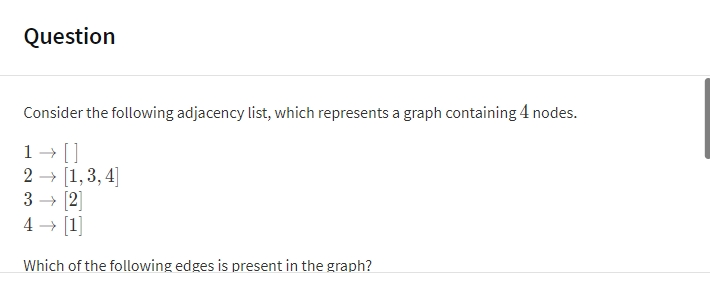
\includegraphics[width=\textwidth]{graphquestion2-1.png}
\end{figure}

\begin{figure}[H]
    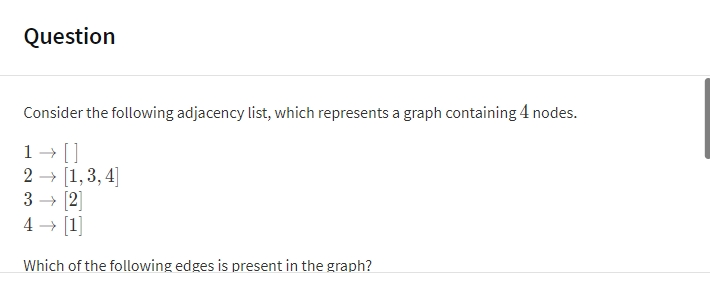
\includegraphics[width=\textwidth]{graphquestion2-1.png}
\end{figure}

\subsection{Graph Traversals and Breadth First Traversal}

\paragraph{
    There are two common ways to traverse a graph: breadth-first traversal and depth-first traversal.\\
    In a breadth-first traversal, we start at a vertex and visit all of its neighbors before moving on to the next level of neighbors.\\
    In a depth-first traversal, we start at a vertex and visit one of its neighbors, then visit one of the neighbor's neighbors, and so on, until we reach a dead end.\\
    Then we backtrack and visit another neighbor of the original vertex.\\
    Breadth-first traversal/Search is useful for finding the shortest path between two vertices in an unweighted graph.\\
    Depth-first traversal is useful for finding cycles in a graph.\\
    Here is an example of a breadth-first traversal of a graph.\\
}

\begin{figure}[H]
    \includegraphics[width=\textwidth]{breadthfirsttraversal.png}
    \caption{Queue: FIFO(First In First Out)}
\end{figure}

\paragraph{
    Here is an indepth explanation of BFS (Breadth-first Search/Traversal). 
    https://blog.csdn.net/g11d111/article/details/76169861.
    In a simple way, BFS is a traversal algorithm that goes through the graph in a wide range before going deep into the graph further(Neighbors First).\\
    On the other side, the depth-first traversal goes into the graph deeply from one neighbor of the starting point before going through 
    another neighbor.\\
}


\subsection{Depth First Search}

\paragraph{
    Depth-first search is a graph traversal algorithm that starts at a vertex and explores as far as possible along each branch before backtracking.\\
    It is similar to the way we would explore a maze, where we would go down one path until we reach a dead end, then backtrack and try another path.\\
    Depth-first search is useful for finding cycles in a graph.\\
    Here is an example of a depth-first search of a graph.\\
}

\begin{figure}[H]
    \includegraphics[width=\textwidth]{depthfirstsearch.png}
    \caption{Stack: LIFO(Last In First Out)
        The stack is used to store the nodes that we have visited but have not yet explored all of their neighbors.\\
        When we visit a node, we push it onto the stack.\\
        When we finish exploring all of the neighbors of a node, we pop it off the stack.\\    
    }
\end{figure}

\paragraph{
    When we go through DFS, we will visit all the successors from one neighbor of the root node first.\\
    Then we will go back to the root node.\\
    While doing this, if any of the visited nodes have other successors that have not been visited, we will visit them first.\\
    This is the main difference between BFS and DFS.\\
}

paragraph{Here is a pseudo code in order to loop through a function dfsVisit(), which apparently deals with dfs.\\
    there is a very subtle technical issue in this pseudo-code: it has to do with setting v.seen = TRUE before dfsVisit(G, v). \\
    Please read the pseudo code for the main loop as }


\begin{verbatim}
    dfs(G)
        for each vertex v in G:
            v.d = Nil #dicovery time
            v.pi = Nil #parrent
            v.seen = FALSE
        time = 0
        for each vertex v in G:
            if v.d = Nil:
                v.d = time
                time = time + 1
                dfsVisit(G, v)
                v.seen = TRUE
\end{verbatim}

\paragraph{
    What is a DFS Tree?\\
    A DFS tree is a tree that is created by a depth-first search of a graph.\\
    It is a subgraph of the original graph that contains all the vertices and edges that are visited 
    during the depth-first search.\\
    It is directed, where each edge points from a parent vertex to a child vertex.\\
    And what is a back edge?\\
    A back edge is an edge that connects a vertex to one of its ancestors in the DFS tree. 
    It may connect back to their grandparent, grand-grandparent and so on.\\
    It is a cycle in the graph.\\
    If we encounter a back edge during a depth-first search, we know that the graph contains a cycle.\\
}

TBD 16:16























\end{document}